
%% bare_jrnl_compsoc.tex
%% V1.4b
%% 2015/08/26
%% by Michael Shell
%% See:
%% http://www.michaelshell.org/
%% for current contact information.
%%
%% This is a skeleton file demonstrating the use of IEEEtran.cls
%% (requires IEEEtran.cls version 1.8b or later) with an IEEE
%% Computer Society journal paper.
%%
%% Support sites:
%% http://www.michaelshell.org/tex/ieeetran/
%% http://www.ctan.org/pkg/ieeetran
%% and
%% http://www.ieee.org/

\documentclass[10pt,journal,compsoc]{IEEEtran}
%
% If IEEEtran.cls has not been installed into the LaTeX system files,
% manually specify the path to it like:
% \documentclass[10pt,journal,compsoc]{../sty/IEEEtran}

% *** CITATION PACKAGES ***
%
\ifCLASSOPTIONcompsoc
% IEEE Computer Society needs nocompress option
% requires cite.sty v4.0 or later (November 2003)
\usepackage[nocompress]{cite}
\else
% normal IEEE
\usepackage{cite}
\fi

% *** GRAPHICS RELATED PACKAGES ***
%
\ifCLASSINFOpdf
  \usepackage[pdftex]{graphicx}
  % declare the path(s) where your graphic files are
  % \graphicspath{{../pdf/}{../jpeg/}}
  % and their extensions so you won't have to specify these with
  % every instance of \includegraphics
  % \DeclareGraphicsExtensions{.pdf,.jpeg,.png}
\else
  % or other class option (dvipsone, dvipdf, if not using dvips). graphicx
  % will default to the driver specified in the system graphics.cfg if no
  % driver is specified.
  % \usepackage[dvips]{graphicx}
  % declare the path(s) where your graphic files are
  % \graphicspath{{../eps/}}
  % and their extensions so you won't have to specify these with
  % every instance of \includegraphics
  % \DeclareGraphicsExtensions{.eps}
\fi
\usepackage{booktabs} % For formal tables
\usepackage{algorithm}
\usepackage{algorithmicx}
\usepackage{algpseudocode}
\usepackage{listings}
\usepackage{xcolor}
\usepackage{setspace}
\usepackage{balance}
\usepackage{color}
\usepackage{soul}

\usepackage{tikz}
\usepackage{amsmath}
\usepackage{multirow}

\floatname{algorithm}{Algorithm}

\newcommand{\tabincell}[2]{\begin{tabular}{@{}#1@{}}#2\end{tabular}}

% correct bad hyphenation here
\hyphenation{op-tical net-works semi-conduc-tor}


\begin{document}
%
% paper title
% Titles are generally capitalized except for words such as a, an, and, as,
% at, but, by, for, in, nor, of, on, or, the, to and up, which are usually
% not capitalized unless they are the first or last word of the title.
% Linebreaks \\ can be used within to get better formatting as desired.
% Do not put math or special symbols in the title.
\title{A Structure-aware Storage Optimization for Out-of-Core Concurrent Graph Processing}
%
%
% author names and IEEE memberships
% note positions of commas and nonbreaking spaces ( ~ ) LaTeX will not break
% a structure at a ~ so this keeps an author's name from being broken across
% two lines.
% use \thanks{} to gain access to the first footnote area
% a separate \thanks must be used for each paragraph as LaTeX2e's \thanks
% was not built to handle multiple paragraphs
%
%
%\IEEEcompsocitemizethanks is a special \thanks that produces the bulleted
% lists the Computer Society journals use for "first footnote" author
% affiliations. Use \IEEEcompsocthanksitem which works much like \item
% for each affiliation group. When not in compsoc mode,
% \IEEEcompsocitemizethanks becomes like \thanks and
% \IEEEcompsocthanksitem becomes a line break with idention. This
% facilitates dual compilation, although admittedly the differences in the
% desired content of \author between the different types of papers makes a
% one-size-fits-all approach a daunting prospect. For instance, compsoc
% journal papers have the author affiliations above the "Manuscript
% received ..."  text while in non-compsoc journals this is reversed. Sigh.

%////////////////////////////////////
\author{Xiaofei~Liao,~\IEEEmembership{Member,~IEEE,}
	~Jin~Zhao,
	~Yu~Zhang,~\IEEEmembership{Member,~IEEE,}
	~Bingsheng~He,~\IEEEmembership{Member,~IEEE,}
	~Ligang~He,~\IEEEmembership{Member,~IEEE,}
	~Hai~Jin,~\IEEEmembership{Fellow,~IEEE,}
	~Lin~Gu,~\IEEEmembership{Member,~IEEE}
	\IEEEcompsocitemizethanks{\IEEEcompsocthanksitem Xiaofei Liao, Jin Zhao, Yu Zhang (Corresponding author), Hai Jin, and Lin Gu are with National Engineering Research Center for Big Data Technology and System, Service Computing Technology and System Lab, Cluster and Grid Computing Lab, School of Computer Science and Technology, Huazhong University of Science and Technology, Wuhan, 430074, China. \protect\\
		E-mail: \{xfliao, zjin, zhyu, hjin, lingu\}@hust.edu.cn
		\IEEEcompsocthanksitem Bingsheng He is with the Department of Computer Science, National University of Singapore, Singapore 117418. \protect\\
		E-mail: hebs@comp.nus.edu.sg
		\IEEEcompsocthanksitem Ligang He is with the Department of Computer Science, University of Warwick, Coventry CV4 7AL, United Kingdom.\protect\\
		E-mail: liganghe@dcs.warwick.ac.uk
	}
}

% The paper headers
%////////////////////////////////////
\markboth{IEEE TRANSACTIONS ON COMPUTERS,~Vol.~X, No.~X, January~2021}%
{Shell \MakeLowercase{\textit{Liao et al.}}: A Structure-aware Storage Optimization for Out-of-Core Concurrent Graph Processing}

\IEEEtitleabstractindextext{%
\begin{abstract}
With the huge demand for graph analytics in many real-world applications, massive iterative graph processing jobs are concurrently performed on the same graphs and suffer from significant high data access cost.
To lower the data access cost toward high performance, several out-of-core concurrent graph processing solutions are recently designed to handle concurrent jobs by enabling these jobs to share the accesses of the same graph data.
However, the set of active vertices in each partition are usually different for various concurrent jobs and also evolve with time, where some high-degree ones (or called {\em hub-vertices}) of these active vertices require more iterations to converge due to the power-law property of real-world graphs.
In consequence, existing solutions still suffer from much unnecessary I/O traffic, because they have to entirely load each partition into the memory for concurrent jobs even if most vertices in this partition are inactive and may be shared by a few jobs.
In this paper, we propose an efficient structure-aware storage system, called GraphSO, for higher throughput of the execution of concurrent graph processing jobs.
It can be integrated into existing out-of-core graph processing systems to promote the execution efficiency of concurrent jobs with lower I/O overhead.
The key design of GraphSO is a fine-grained storage management scheme.
Specifically, it logically divides the partitions of existing graph processing systems into a series of small same-sized chunks.
At runtime, these small chunks with active vertices are judiciously loaded by GraphSO to construct new logical partitions (i.e., each logical partition is a subset of active chunks) for existing graph processing systems to handle, where the most-frequently-used chunks are preferentially loaded to construct the logical partitions and the other ones are delayed to wait to be required by more jobs.
In this way, it can effectively spare the cost of loading the graph data associated with the inactive vertices with low repartitioning overhead and can also enable the loaded graph data to be fully shared by concurrent jobs.
Moreover, GraphSO also designs a buffering strategy to efficiently cache the most-frequently-used chunks in the main memory to further minimize the I/O traffic by avoiding repeated load of them.
Experimental results show that GraphSO improves the throughput of GridGraph, GraphChi, X-Stream, DynamicShards, LUMOS, Graphene, and Wonderland by 1.4-3.5 times, 2.1-4.3 times, 1.9-4.1 times, 1.9-2.9 times, 1.5-3.1 times, 1.3-1.5 times, and 1.3-2.7 times after integrating with them, respectively.

\end{abstract}

% Note that keywords are not normally used for peerreview papers.
\begin{IEEEkeywords}
Iterative graph processing, out-of-core, concurrent jobs, storage system
\end{IEEEkeywords}}


% make the title area
\maketitle


% To allow for easy dual compilation without having to reenter the
% abstract/keywords data, the \IEEEtitleabstractindextext text will
% not be used in maketitle, but will appear (i.e., to be "transported")
% here as \IEEEdisplaynontitleabstractindextext when the compsoc
% or transmag modes are not selected <OR> if conference mode is selected
% - because all conference papers position the abstract like regular
% papers do.
\IEEEdisplaynontitleabstractindextext
% \IEEEdisplaynontitleabstractindextext has no effect when using
% compsoc or transmag under a non-conference mode.



% For peer review papers, you can put extra information on the cover
% page as needed:
% \ifCLASSOPTIONpeerreview
% \begin{center} \bfseries EDICS Category: 3-BBND \end{center}
% \fi
%
% For peerreview papers, this IEEEtran command inserts a page break and
% creates the second title. It will be ignored for other modes.
\IEEEpeerreviewmaketitle

\IEEEraisesectionheading{\section{Introduction}\label{sec:introduction}}
%\IEEEPARstart{I}{n} the past decade, graphs have been widely used as the preferred data representation to capture relationships between entities in many fields such as social networks, web graphs, e-commerce user-item graphs, etc. It allows data analysts to exploit valuable information from patterns in the graph data for many application domains, including machine learning~\cite{Tux,NeuGraph}, clustering~\cite{ShunRFM16,LiuJH19}, recommendation~\cite{FoussPRS07,GuanBMCW09}, social influence analysis~\cite{LiuLS20,WangCZXJHDL11}.

\IEEEPARstart{W}{ith} the huge demand for analyzing graph data, massive concurrent iterative graph processing jobs are often executed on the common platforms (e.g., Giraph~\cite{Giraph}, Pregel~\cite{Pregel}, GraphJet~\cite{GraphJet}, and Plato~\cite{Knightking,Gemini}) of many enterprises (e.g., Facebook~\cite{facebook}, Google~\cite{Google}, Twitter~\cite{twitter_web}, and Tencent~\cite{tencent}) daily to exploit various properties of their underlying graphs offline, for different applications (e.g., the variants of PageRank~\cite{PageRank} for content recommendation, WCC~\cite{SCC} for social media monitoring, and $k$-means~\cite{k-means} for customer segmentation). Fig.~\ref{number_jobs} shows the number of jobs that are running concurrently on a common graph processing platform of a real Chinese social network. There can be up to 30 concurrent graph processing jobs.
Although many out-of-core graph processing systems, e.g., X-stream~\cite{X-stream}, GridGraph~\cite{GridGraph}, and DynamicShards~\cite{Vora}, are proposed to efficiently handle a single job with high cost efficiency, they surfer from much redundant I/O cost since the same graph data are repeatedly loaded to serve concurrent jobs.
Thus, several recent studies~\cite{seraph,CGraph,GraphM,seraph1,CGraph2019} propose to eliminate the redundant I/O traffic by enabling concurrent jobs to share the storage and accesses of the same graph.
These solutions first divide the graphs into static partitions to reside in the disk, where each partition consists of a number of vertices and their associated edges.
During execution, the active static partition (i.e., its vertices are active for some jobs) is loaded into the memory in some special ways to serve concurrent jobs for less data access cost.


\begin{figure}[!t]
	\begin{minipage}[t]{0.48\textwidth}
		\centering
		%\vspace{-0.2cm}
		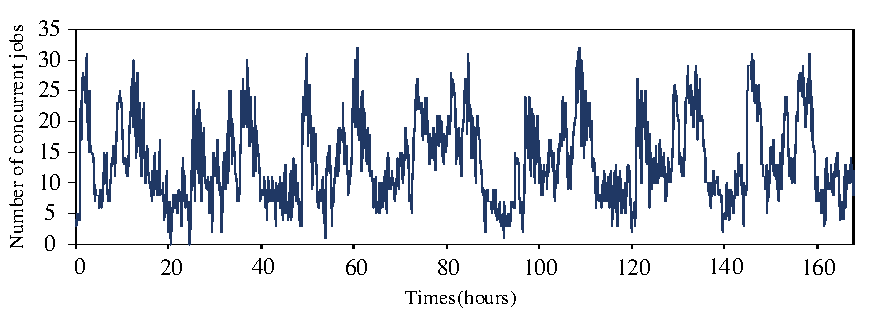
\includegraphics[width=3.5in]{number_jobs.pdf}
		\vspace{-28pt}
		\caption{Number of jobs traced on a social network}
		%Percentage of the graph shared by various number of jobs over time}
		\label{number_jobs}
	\end{minipage}
	\vspace{-18pt}
\end{figure}

%However, own much higher degrees than the other vertices

However, with these solutions~\cite{seraph,seraph1,CGraph,CGraph2019,GraphM}, each active partition (i.e., some vertices and edges in this partition need to be processed by a job) needs to be loaded into the memory, even when the most proportion of the vertices and edges of this partition are not needed by any job or are only needed by a few jobs.
In fact, the set of active vertices are usually different for various concurrent jobs and also evolve over time because of their various parameters and different computational complexity. Besides, a few vertices (or called {\em hub-vertices}) require more iterations to converge than other vertices because of the power-law property~\cite{PowerGraph} of the real-world graphs, which causes a large number of vertices in each active static partition to be inactive for most concurrent jobs at most iterations.
Repeatedly loading the graph data associated with these inactive vertices leads to severe I/O inefficiency and also causes the loaded graph data to be shared by only a few concurrent jobs. It eventually incurs low throughput of concurrent jobs.


To tackle this challenge, in this paper,
we propose a structure-aware storage system {\em GraphSO}
$\footnote{The source code of GraphSO is available at: https://github.com/Program-Anonymity/GraphSO.git}$
for concurrent graph processing jobs.
Through the provided APIs, GraphSO can be integrated into existing out-of-core graph processing systems to efficiently handle concurrent iterative graph processing jobs, without modifying the applications on these systems.
Specifically, GraphSO logically divides the static partitions into a series of small same-sized chunks for fine-grained management of the graph storage.
At runtime, only the chunks with active vertices are judiciously loaded by GraphSO to construct new logical partitions with the suitable size required by existing graph processing system.
In this way, it can efficiently reduce the unnecessary I/O overhead resulted from loading the graph data associated with the inactive vertices of the active static partitions.
Because some chunks (e.g., the ones required by more jobs or with more hub-vertices) may need to be repeatedly processed by concurrent jobs at many iterations, these chunks are preferentially loaded to construct the logical partitions to serve the execution of the concurrent jobs. The other ones are delayed so as to make them wait to be required by more jobs.
It enables the generated logical partitions to be reused by as many jobs as possible.
After that, each generated logical partition is handled by concurrent jobs in a novel synchronous way. Only when a chunk of the generated logical partition has been handled by the related jobs, the next chunk can be processed.
When all chunks of a logical partition have been handled, the next logical partition can be generated for processing.
By doing so, it can regularly stream the chunks into the main memory and the \textit{Last-Level Cache} (LLC) to maximize the chunk reuse in the main memory and the LLC, to lower the data access cost.
Finally, GraphSO tries to cache the frequently-used chunks in the main memory via a structure-aware buffering strategy, which can further minimize the I/O traffic by eliminating the repeated I/Os for loading these chunks.


This paper mainly owns the following contributions:
\vspace{-4pt}
\begin{itemize}
\vspace{-1pt}
\item We disclose the significant I/O inefficiencies of existing out-of-core concurrent graph processing solutions and observe that it is the main problem that slows down overall performance.
\vspace{-1pt}
\item We propose a structure-aware storage system that enables existing out-of-core graph processing systems to efficiently and effectively handle concurrent jobs by reducing the unnecessary I/O traffic and maximizing the utilization of the loaded graph data.
\item We design a structure-aware buffering strategy to further minimize I/O overhead.
\vspace{-1pt}
\item We integrate GraphSO into seven popular out-of-core graph processing systems, i.e., GridGraph~\cite{GridGraph},  GraphChi~\cite{GraphChi}, X-Stream~\cite{X-stream}, DynamicShards~\cite{Vora}, LUMOS~\cite{LUMOS}, Graphene~\cite{Graphene}, and Wonderland~\cite{Wonderland}. Extensive results show that GraphSO can improve the throughput of concurrent jobs by 1.4-3.5 times, 2.1-4.3 times, 1.9-4.1 times,  1.9-2.9 times, 1.5-3.1 times, 1.3-1.5 times, and 1.3-2.7 times for GridGraph, GraphChi, X-Stream, DynamicShards, LUMOS, Graphene, and Wonderland, respectively.
\vspace{-4pt}
\end{itemize}

The remainder is organized as below. The I/O inefficiencies of existing solutions are discussed in Section~\ref{sec:2}. Section~\ref{sec:3} presents the system design and the implementation of GraphSO. Section~\ref{section:Evaluation} describes the experimental evaluation. The related works are reviewed in Section~\ref{sec:5}. Finally, this work is concluded in Section~\ref{sec:6}.

% We discuss the related works in Section 5 and conclude this paper in Section 6.

\begin{figure}[!t]
	\centering
	%\vspace{-12pt}
	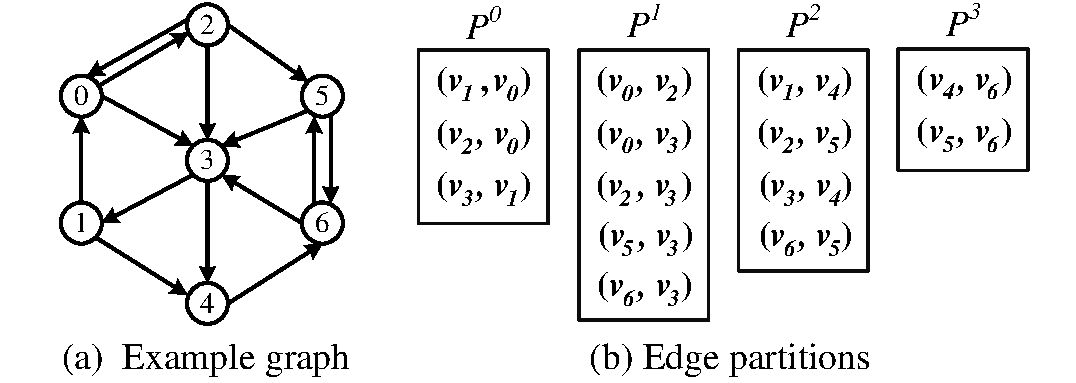
\includegraphics[width=3.3in]{graph.pdf}
	\vspace{-15pt}
	\caption{Example to divide a graph into four static partitions ($P^0$, $P^1$, $P^2$, and $P^3$) that reside on disk}
	\label{graph}
	\vspace{-17pt}
\end{figure}

\vspace{-10pt}
\section{Background and Motivation}\label{sec:2}
%This section first introduces the out-of-core concurrent graph processing systems, and then explains our observations on the I/O inefficiency when existing systems handle concurrent graph processing jobs.

\vspace{-2pt}
\subsection{Out-of-Core Concurrent Graph Processing}
\vspace{-2pt}
Recently, several solutions~\cite{CGraph,GraphM} are proposed to enable multiple iterative graph algorithms to concurrently analyze the same large real-world graphs for high performance efficiency on a single machine.
The graph data for each iterative graph processing job consist of the job-specific vertex value data (i.e, $S$), e.g., the distances from source vertex for SSSP~\cite{SSSP} and the ranking scores for PageRank~\cite{PageRank}, and the graph structure data (i.e., $G$).
To get better performance, existing solutions enable the storage and data accesses of $G$ to be shared by concurrent jobs because $G$ is the same for these jobs. Specially, the graph structure data are first partitioned into static partitions, which are usually first stored on the disk.
Fig.~\ref{graph} depicts an example graph partitioned into four static partitions, and each of which is comprised of a subset of vertices along with these vertices' incoming edges.
Within each iteration, the active static partitions for each job are first identified, and the intersection of these partitions for different jobs is then derived.
%TODO %% who are they?
After that, the shared static partitions can be gotten for concurrent jobs and are sequentially loaded to serve these jobs. To exploit the sequential performance of disk, existing solutions usually entirely load each static partition into the memory. After processing all of the active static partitions, the vertex value data of these jobs will be updated and the active static partitions that need to be processed at the next iteration of each job can be obtained. Note that the static partitions will be repeatedly traversed to serve concurrent jobs until all static partitions become inactive for these jobs.

\vspace{-10pt}
\subsection{Inefficiency of I/O Performance}
\vspace{-2pt}
While the above solutions leverage disk locality, it suffers from much unnecessary overhead. During the execution, the static partitions may contain both active and inactive vertices.
Entirely loading each static partition within every iteration incurs the useless effort for loading and processing the graph data associated with inactive vertices. This wasteful effort is the main reason to slow down the overall performance because (1) the concurrent graph processing cost is dominated by graph data accessing, and (2) at the most iterations, a large proportion of vertices in the static partitions are inactive for concurrent jobs.
Fig.~\ref{IO_inefficient}~(a) depicts the execution time breakdown for concurrent jobs on the cutting-edge out-of-core concurrent graph processing system called GridGraph-M (i.e., GridGraph~\cite{GridGraph} integrated with GraphM~\cite{GraphM}) over five real-world graphs. The benchmarks and platform will be introduced in detail in Section~\ref{section:4.1}. From Fig.~\ref{IO_inefficient} (a), we can find that the graph data accessing time occupies a large ratio of total execution time, and the ratio increases as the graph size becomes larger.
To understand how much unnecessary I/O overhead is incurred, we evaluate the percentages of the loaded inactive edges (i.e., the loaded edges with inactive source vertices) to the total loaded edges for concurrent jobs on GridGraph-M. As depicted in Fig.~\ref{IO_inefficient}~(b), there indeed exists significantly unnecessary I/O overhead. For example, over \textit{CW}, GridGraph-M takes over 86\% I/O traffic to load the inactive edges for concurrent jobs.

\begin{figure}[!t]
	\centering
	%\vspace{-12pt}
	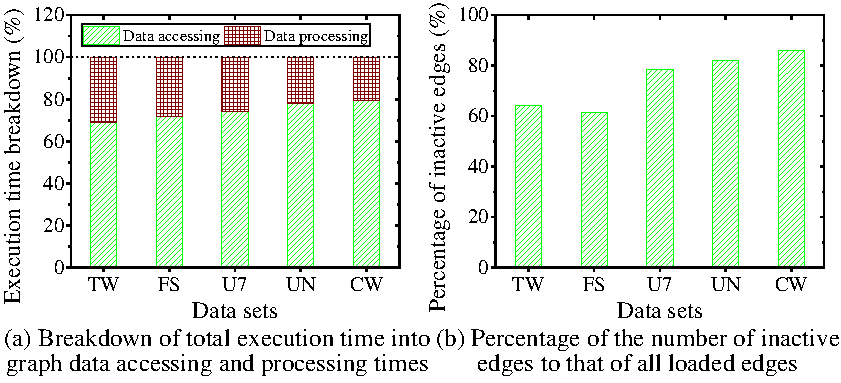
\includegraphics[width=3.4in]{IO_inefficient.pdf}
	\vspace{-12pt}
	\caption{The execution statistics of concurrent jobs: (a) Breakdown the total execution time into graph accessing and graph processing times, (b) Percentage of inactive edges to total loaded edges during the execution.}
	\label{IO_inefficient}
	\vspace{-12pt}
\end{figure}

\begin{figure}[!t]
	\centering
	%\vspace{-12pt}
	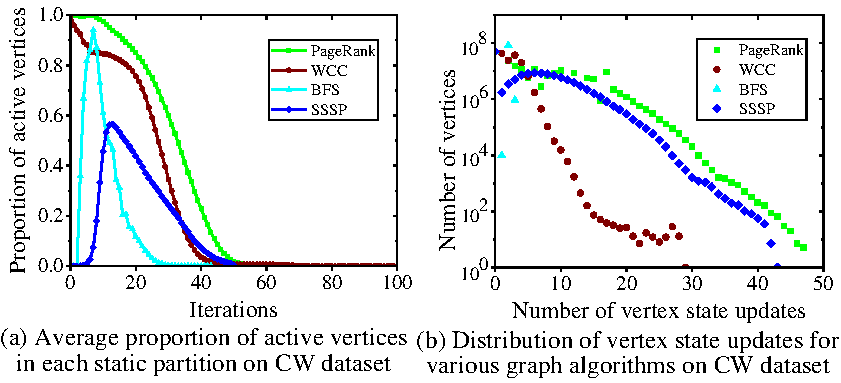
\includegraphics[width=3.4in]{active_ratio_times.pdf}
	\vspace{-12pt}
	\caption{(a) average proportion of the number of active vertices to that of vertices in each active static partition for jobs over CW dataset, (b) distribution of the number of vertex state updates for jobs in CW dataset, where the vertices are sorted by the number of their updates.}
	\label{active_ratio_times}
	\vspace{-12pt}
\end{figure}

We attribute these phenomena to the real-world graphs' power-law property~\cite{PowerGraph}. Specifically, a small part of vertices (called hub-vertices) are neighbored with most vertices.
Generally, hub-vertices require more iterations to converge than others, because their values are impacted by most vertices.
Thus, only a small part of vertices in the static partitions are active for concurrent jobs after a few iterations.
To prove this phenomena, we evaluated the details of the data accesses characteristic of concurrent jobs on GridGraph-M over CW dataset.
Fig.~\ref{active_ratio_times}(a) depicts the average proportion of the number of active vertices to that of vertices in each partition across iterations in different algorithms.
We can observe that the ratio of active vertices drops significantly after a few iterations and becomes very low as the algorithms close to convergence. Besides, the active vertices are different for various algorithms in each iteration and evolve with time.
Fig.~\ref{active_ratio_times}(b) depicts the distribution of the number of vertex state updates when performing different algorithms.
It shows that a few vertices are frequently handled by concurrent jobs than others, because these vertices connect with most vertices.
Thus, the most ratio of the I/O traffic is carried out for loading the graph data associated with these vertices.
It motivates us to propose a structure-aware graph storage optimizations based on the set of active vertices of the concurrent jobs to solve the I/O inefficiency of concurrent jobs for higher throughput.

\vspace{-10pt}
\section{Design of GraphSO}\label{sec:3}
\vspace{-2pt}
The structure-aware storage system proposed in this paper is named GraphSO. By using several APIs provided by GraphSO, it can be integrated into existing out-of-core graph processing systems to efficiently manage the storage and data access of the same graph for concurrent jobs. First, it logically divides the static partitions into fine-grained chunks so as to provide an opportunity to transparently minimize the unnecessary I/O overhead.
After that, it judiciously loads the active chunks to repartition them into the logical partitions to serve the execution of concurrent jobs.
In this way, the graph data associated with many inactive vertices in the static partitions do not need to be loaded along with the active ones in these static partitions, and the generated logical partitions can be fully shared by concurrent jobs.
%Next, a scheduling scheme is proposed to enable  to be  through judiciously assigning the logical partition loading order.
Finally, the frequently-used chunks are buffered in the memory to further reduce I/O traffic. %Moreover,  for integrating GraphSO with existing out-of-core graph processing systems.
%and illustrated how to use them in existing systems.

\vspace{-10pt}
\subsection{Overview of GraphSO}
\vspace{-2pt}
Fig.~\ref{Architectural} shows the architecture of GraphSO, and its key techniques mainly include structure-aware adaptive graph repartitioning/processing and structure-aware buffering. %, which are overviewed as follows.


\textit{Structure-aware Adaptive Graph Repartitioning and Processing.} Before the execution, the graph data usually needs to be preprocessed.
The partitioning methods and graph formats for different graph processing systems are usually varied. Therefore, for each graph processing system integrated with GraphSO, the original graph stored in GraphSO is first divided into static partitions according to the partitioning methods of this system, and then the static partitions are respectively converted into the graph format adopted in the graph processing system (e.g., the grid format for GridGraph~\cite{GridGraph} and the shard format for GraphChi~\cite{GraphChi}).
%Note that it dose not modify the specific graph format.
We do not modify the graph format used by any graph processing systems for transparent integration of GraphSO.
The static partitions are then stored in the disk.
To achieve fine-grained graph management (i.e., graph repartitioning and buffering) as the following described, the static partitions are logically divided into small same-sized chunks, and the information of the small chunks are stored in a \textit{TChunk} table. Each chunk should be fit in the LLC to exploit the cache locality.

After that, the graph data needs to be loaded into the memory to serve the execution of concurrent jobs.
To reduce the unnecessary I/O for loading the unnecessary graph data, it identifies the active chunks (i.e., $C_{active}$) before each iteration.
Then, GraphSO logically repartitions the graph by loading and assigning the active chunks together to construct the logical partitions to serve concurrent jobs.
Note that the important chunks (e.g., the ones are required by more jobs or own many hub-vertices) are distinguished and preferentially loaded by GraphSO to generate the logical partitions, enabling the generated logical partitions can be shared by more jobs. The other chunks are delayed to wait to be required by more jobs.
%To , a scheduling scheme is proposed to assign their loading order. In detail, the logical partitions, which contain many important chunks, are first loaded into the memory.
%This repartitioning function is designed as an API as: $LP$$\leftarrow$$Repartition$($C_{active}$, $|P|$)), where $LP$ is the constructed logical partitions and $|P|$ is the size of the static partitions required by the related graph processing system. Besides, the important chunks (e.g., the ones own many hub-vertices) are distinguished and allocated together to reduce the repartitioning cost.
%After repartitioning, the logical partitions can be loaded into the memory.
This procedure is drafted as an API as: $LP^i_j$$\leftarrow$$Schedule$($C_{active}$, $|P|$, $Load$()), where $|P|$ is the size of the static partitions required by the related graph processing system,
%$LP$ is the set of logical partitions that need to be loaded,
$LP^i_j$ is the generated logical partition in the memory and is loaded by job~\textit{j}. $LP^i_j$ can be shared by its related jobs (the ones need to handle it), and the unrelated jobs are suspended until their active partitions are loaded.
Note that the next logical partition can be generated to be handled by concurrent jobs only if the generated logical partition has been processed by all of its related jobs.

\begin{figure}[!t]
	\centering
	%\vspace{-0.3cm}
	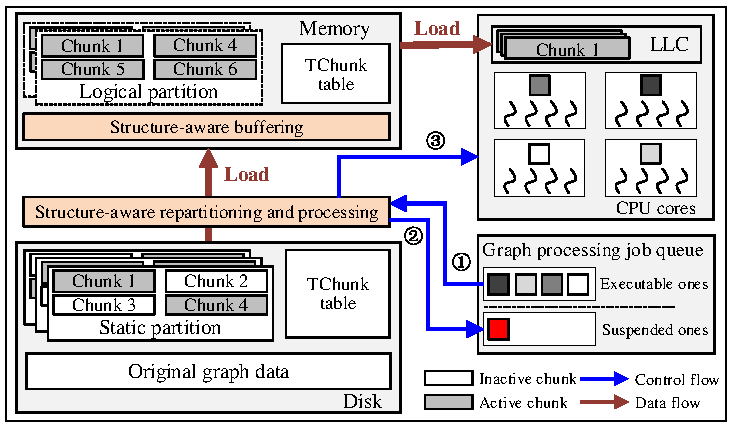
\includegraphics[width=3.5in]{Architectural.pdf}
	\vspace{-20pt}
	\caption{The architecture of GraphSO}
	\label{Architectural}
	\vspace{-20pt}
\end{figure}

%\textit{Structure-aware Scheduling and Processing.}

Besides, the workload of each logical partition is usually skewed between various jobs because of their different active vertex number and computational complexity. Thus, when processing each generated partition, it unevenly allocates the computing resources to concurrent jobs so as to synchronously handle each chunk in the LLC.
In this way, each chunk can be reused by different jobs when it is loaded into the LLC, in order to lower the data access cost.
Note that, although the important chunks may be loaded for the concurrent jobs multiple times, each job handles the loaded chunks only if this job needs to process this loaded chunks at this moment. Therefore, GraphSO does not affect the correctness of the final results of each job.

\textit{Structure-aware Buffering.} To further reduce the data access cost and fully utilize the memory resources, several chunks are selected and cached in the main memory. In detail, the important chunks need to be preferentially cached in the memory because of their higher loading frequency during the execution. %Besides, the other chunks may be repeatedly handled by concurrent jobs in several contiguous iterations.
Thus, a buffering strategy is designed to preferentially cache the important chunks for the concurrent jobs.
In this way, the repetitive I/O traffic for loading the cached chunks can be reduced for concurrent jobs.

\textit{Programming APIs.} To transparently use GraphSO, several APIs need to be inserted into existing graph processing systems, while the graph applications executed on these systems do not need to be modified. Specifically, $Init()$ is adopted to initialize GraphSO through dividing the static partitions into the fine-grained chunks as discussed in Section~\ref{section:3.2}. $GetActiveChunks()$ and $Schedule()$ are inserted between successive iterations in the program to get the active chunks and efficiently load the generated logical partitions for the concurrent jobs, respectively. Note that, $GetActiveChunks()$ needs to be placed before $Schedule()$ to identify the active chunks for graph repartitioning.

%replaces the original graph load operation for efficiently loading the logical partitions to be shared by concurrent jobs.

\vspace{-8pt}
\subsection{Repartition-centric Execution of Concurrent Jobs}\label{section:Repartitioning}
\vspace{-2pt}
In most iterations, there may be only a few vertices that are active for concurrent jobs due to the power-law property~\cite{PowerGraph}, incurring much unnecessary I/O traffic for loading the graph data associated with the inactive vertices in each static partition.
Although some solutions~\cite{Vora, ReGraph} are proposed to dynamically repartition the graph, the set of active vertices is usually different for various jobs and the number of the related jobs of different active vertices is usually skewed.
%Therefore, with existing solutions, 
%most proportion of the dynamic partitions may be shared by only a few jobs.
%The layout of the same underlying graph may even become different for various jobs.
%It makes the same graph data unable to be efficiently shared by the concurrent jobs and these jobs have to individually maintain multiple copies of the same graph data.
%Besides, each job also suffers from high overhead to repartition the graph individually.
Therefore, when using existing solutions~\cite{Vora, ReGraph} to support the execution of the concurrent jobs, the graph will be repartitioned individually and gets different repartitioned results for different jobs. It incurs high repartitioning cost. Furthermore, the layouts of the same underlying graph are different for different jobs, and thus multiple copies of the same graph have to be accessed and maintained for these jobs individually. In addition, when integrating existing repartitioning solutions~\cite{Vora, ReGraph} into the existing concurrent graph processing systems (e.g., GraphM~\cite{GraphM}) to serve multiple concurrent jobs, the frequently accessed active vertices (i.e., the ones to be processed by much more concurrent jobs) may be repartitioned together with the other infrequently accessed active vertices (i.e., the ones to be processed by only a few concurrent jobs or even only one job). 
It causes low utilization of the loaded dynamic partitions and also high repartitioning overhead.

To address the above problems, we propose a structure-aware adaptive graph repartitioning and processing scheme to efficiently serve the execution of concurrent jobs.
Specifically, it first divides the static partitions of existing graph processing systems into fine-grained chunks so as to provide an opportunity to effectively reduce the unnecessary I/O traffic efficiently.
After that, at the execution time, the set of active chunks are dynamically identified and
adaptively repartitioned into the common logical partitions for different concurrent jobs, and then trigger these jobs to synchronously handle these logical partitions. Thereby, it enables these jobs to effectively share the repartitioned results and the accesses to the same graph data.
Note that, the most-frequently-used chunks are tried to be assigned into the same logical partitions together, which enables the logical partitions to be fully shared by the concurrent jobs. %sparing the storage and data access cost.
It enables higher utilization of the loaded graph data and also much lower repartitioning cost.

\vspace{-10pt}
\subsubsection{Fine-grained Graph Representation}\label{section:3.2}
\vspace{-2pt}
To achieve fine-grained graph management, the static graph partitions need to be logically divided into small chunks.
When using the existing fine-grained partitioning strategy~\cite{GraphChi,GridGraph,Graphene}, it may cause much redundant data access cost or high synchronization overhead for processing each chunk.
Specifically, if the chunk size is larger than the LLC size, it causes much redundant data access cost, because of cache thrashing and intense contention among concurrent jobs. If the chunk size is too small, it may cause frequent synchronization among the concurrent jobs, because the next chunk is allowed to be loaded by GraphSO only if the concurrent jobs have processed the current chunk.
Therefore, for better cache locality and higher system performance,
the suitable chunk size (i.e., $\left|C\right|$) should fit into that of the LLC. Thus, the value of $|C|$ is determined by:
\vspace{-4pt}
\begin{equation}
\label{eq:chunksize}
\vspace{-1pt}
|C| \times N + \frac{|C|\times N}{|G|} \times N_v \times \left| V \right| + s \le |LLC|,
\vspace{-2pt}
\end{equation}
where $|V|$ denotes the size of vertex value, $|G|$ indicates the size of graph structure data. $N$ and $N_v$ represent the number of CPU cores and graph's vertices, respectively. $|LLC|$ is the LLC's size,  $s$ is the reserved space size. Because each chunk is usually handled by one CPU core, the number of chunks loaded in the LLC equals that of CPU cores (i.e., $|C| \times N$). Note that $|C|$ is set as the largest integer that satisfies~\eqref{eq:chunksize}. With such settings, the same chunk can be reused by all related jobs once it is loaded into the LLC, while incurring low synchronization cost at the same time.

\begin{algorithm}[t]
	\caption{Pseudo Code of Fine-grained Dividing}
	\begin{algorithmic}[1]
		\Procedure{Divide($P^i$, $TChunk^i$, $|C|$)}{}
		\State Initial($TChunk^i$) \label{Initial}
		\State $c \leftarrow 0$ \ /*c indicates the $c^{th}$ chunk in $P^i$*/
		\For{each edge $e$ $\in$ $P^i$}
		\If {$e_s \in TChunk^i_c$} \label{collect1}
		\State $TChunk^i_c.N^+$($e_s$) $\leftarrow TChunk^i_c.N^+$($e_s$) + 1 \label{ADD_N}
		\Else
		\State $TChunk^i_c.$Insert($\left \langle e_s, 1 \right  \rangle$) \label{Inert}
		\EndIf \label{collect2}
		\State $TChunk^i_c.N_e$ $\leftarrow$ $TChunk^i_c.N_e$ + 1
		\If {$TChunk^i_c.N_e$ $\ge$ $\frac{|C|}{|E|}$ or $P^i$ is traversed} \label{a1_11}
		\If {$c$ equals zero} \label{location1}
		\State $TChunk^i_c.Loc$ $\leftarrow$ Location$(P^i)$
		\Else
		\State $TChunk^i_c.Loc$ $\leftarrow$ $TChunk^i_{c-1}.Loc$ + $|C|$
		\EndIf \label{location2}
		%\State /*Prepare to count the edges of next chunk*/ \par\setlength\parindent{4.5em} $num\_edges \leftarrow 0$
		\State $c \leftarrow c+1$\label{Nextchunk}
		\EndIf
		\EndFor
		\EndProcedure
	\end{algorithmic}
	\label{code1}
\end{algorithm}

\begin{figure}[!t]
	\centering
	\vspace{-0.3cm}
	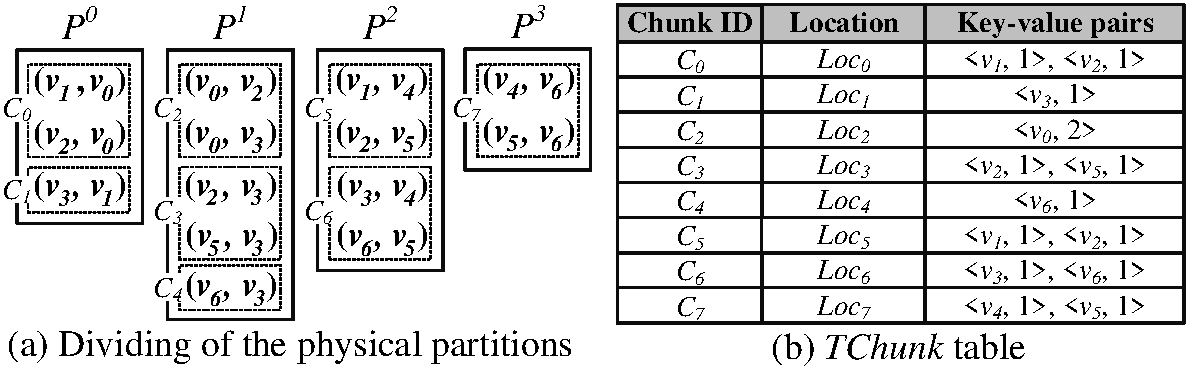
\includegraphics[width=3.5in]{divide.pdf}
	\vspace{-22pt}
	\caption{Illustration of the fine-grained graph dividing, where the example graph partitions are divided into eight chunks and the suitable size of each chunk is assumed to be the total size of two edges}
	\label{divide}
	\vspace{-14pt}
\end{figure}

The static partitions are logically divided into a series of chunks by traversing the graph once, as shown in Fig.~\ref{divide}(a). During the traverse, a \emph{TChunk} table is established to record the information of chunks. Each entry of the \emph{TChunk} table is corresponded to a visited chunk and consists of three fields. As Fig.~\ref{divide}(b) depicts, the first two fields describe the ID and the start location (denoted by $Loc$) of the corresponding chunk in the graph file. The third field is a key-value table to store the source vertices set and the number of their outgoing edges in this chunk. For each key-value pair, the source vertices IDs (e.g., $v_i$) in this chunk are the keys and the number of the vertices' outgoing edges (e.g., $N^+(v_i)$) of this chunk are the values.

The procedure of fine-grained dividing of the static partitions, e.g., $P^i$, is shown in Algorithm~\ref{code1}. The $TChunk^i$ is first initialized to store the information of the chunks in $P^i$ (Line~\ref{Initial}). Then, the edges in $P^i$ are sequentially traversed to collect the edges' source vertices (i.e., $e_s$) and the number of these vertices' outgoing edges (i.e., $N^+(e_s)$) in each chunk (Lines~\ref{collect1}-\ref{collect2}). $TChunk^i_c.N_e$ is used to count the number of edges in chunk \textit{c}. When $TChunk^i_c.N_e$ enables the size of chunk \textit{c} to be the suitable chunk size or all edges in $P^i$ has been traversed (Line~\ref{a1_11}), the start location of chunk \textit{c} (i.e., $TChunk^i_c.Loc$) can be obtained (Lines~\ref{location1}-\ref{location2}). Note that the start location of $P^i$ is set as $TChunk^i_c.Loc$ if chunk $c$ is the first chunk in $P^i$. Then, it moves to store the the next chunk's information (Line~\ref{Nextchunk}). Note that, when the graph is evolved, the consistent snapshots of the concurrent jobs can be maintained by the solution employed in GraphM~\cite{GraphM} and the $TChunk$ also needs to be updated.

\vspace{-6pt}
\subsubsection{Adaptive Graph Repartitioning for Concurrent Jobs}%\label{section:Repartitioning}

%\begin{algorithm}[t]
%	\caption{Pseudo Code of Graph Repartitioning}
%	\begin{algorithmic}[1]
%		\Function{GetLogicalPartition($C_{active}$, $|P|$)}{}
%		\par\setlength\parindent{1.5em} Sort$_{Pri}$($C_{active}$) \label{SortAID}
%		\State $i \leftarrow 0$ \ /*i indicates the $i^{th}$ logical partition $LP^i$*/
%		\For{each chunk $C_m$ $\in$ $C_{active}$} \label{Put1}
%		\If {$|LP^i|$ $\ge$ $|P|$} \label{size}
%		\State $i \leftarrow i+1$
%		\EndIf
%		\State Put chunk $C_m$ into $LP^i$
%		\EndFor  \label{Put2}
%		\For{each logical partition $LP^i$}
%		\State /*Chunks are sorted based on their chunk IDs*/
%		\par\setlength\parindent{3em} Sort$_{ID}$($LP^i$) \label{SortID}
%		\EndFor
%		\State \Return{\textit{LP}} \label{returnLP}
%		\EndFunction
%	\end{algorithmic}
%	\label{code2}
%\end{algorithm}

During the execution, GraphSO dynamically identifies the active chunks for different concurrent jobs. Based on these collected information, GraphSO adaptively repartitions the underlying graph at runtime by judiciously putting the active chunks of all concurrent jobs together into several logical partitions.
These generated logical partitions then are provided to be synchronously handled by all concurrent jobs and can also be shared by them.
By such means, the graph repartitioning cost is amortized by these concurrent jobs and these jobs only need to maintain a single copy of the same underlying graph on the memory and LLC.

In practice, a chunk will be loaded into the memory for processing only if this chunk is active for some jobs (i.e., its vertices are active for these jobs).
Note that, if the vertices of a chunk are updated by some jobs in the current iteration, this chunk can be identified as active chunk for these jobs in the next iteration.
Thus, we can get the active chunks in the next iteration by tracing the vertex update in the current iteration~\cite{G-store}.
In this way, the I/O overhead of loading the inactive chunks in active static partitions can be eliminated.


%After graph repartitioning, all chunks of the same logical partition are loaded from the disk into a contiguous space of main memory to make existing graph processing systems to transparently handle it. However, unsuitable loading order of the logical partitions may incur underutilization of the loaded graph data.
%First, because the hub-vertices are connected with most vertices in the graph, the states of many vertices are affected by that of these hub-vertices. The delayed processing of the logical partitions containing hub-vertices may cause many vertices fail to be activated for these jobs.
%Besides, the logical partitions with more active vertices or associated with more related jobs have a greater impact on vertex state propagation.
%Second, the active vertices and the related jobs are usually different for different logical partitions and are also dynamically changed over time.
%Although existing scheduling strategy~\cite{HotGraph} enables the partitions containing the hub-vertices to be preferentially loaded for processing, it may preferentially load the partition required by a few concurrent jobs or even one job, which causes the loaded data to be shared by a few jobs or even one job.
%Thus, the logical partitions may only be shared by a few jobs or cannot be shared when they are ineffectively loaded into the memory, resulting in poor performance.

\begin{algorithm}[t]
	\caption{Pseudo Code of Repartition-centric Execution}
	\begin{algorithmic}[1]
		\Procedure{Schedule($C_{active}$, $|P|$, $Load()$)}{}
		\State $LP^i \leftarrow$ GenerateLogicalPartition($C_{active}$, $|P|$) \label{getpartition}
		\State $J^i \leftarrow$ GetRelatedJobs($LP^i$) \label{getjobs}
		\State ResumeJob($J^i$)\label{resume}
		\If{$j$$\notin$$J^i$} \label{suspend1}
		\State SuspendJob($j$)
		\EndIf \label{suspend2}
		\State RemoveJob($j$, $J^i$) \label{Remove}
		\State \Return{\textit{$LP^i$}} \label{return}
		\EndProcedure
		
		\Procedure{GenerateLogicalPartition($C_{active}$, $|P|$)}{}
		\State /*Get the top $\frac{|P|}{|C|}$ chunks based on their priorities*/
		\par\setlength\parindent{1.5em} $LP^i$ $\leftarrow$ GetChunks$_{Pri}$($C_{active}$) \label{SortAID}
		\State Sort$_{ID}$($LP^i$) \label{SortID}
		%\State Put chunks $Set_{Chunks}$ into $LP$ \label{Put}
		\If {$LP^i$ has not be loaded into the memory} \label{not}
		\State \textit{Buf} $\leftarrow$ SetSharedBuffer($LP^i$) \label{create}
		\For{each chunk $C_m$$\in$$LP^i$}\label{load1}
		\State \textit{Buf} $\leftarrow$ Load($TChunk_m.Loc$, $TChunk_m.N_e$)
		\EndFor \label{load2}
		\Else
		\State\textit{Buf} $\leftarrow$ ObtainFromSharedBuffer($LP^i$) \label{attach}
		\EndIf
		\State \Return{\textit{Buf}} \label{returnLP}
		\EndProcedure
	\end{algorithmic}
	\label{code3}
\end{algorithm}

Specifically, only the active chunks are expected to be loaded by GraphSO to construct the logical partitions, where the size of each logical graph partition needs to meet the requirement of the integrated graph processing system so as to make GraphSO transparent to the existing graph processing systems. % because the suitable size of the partition (i.e., the static partition size) is different for various graph processing systems.
It is because existing out-of-core graph processing systems~\cite{GridGraph,GraphChi,X-stream,LUMOS} usually load and process the graph data by taking the partition as the basic unit, where the suitable size of the partition (i.e., the static partition size) is determined by the corresponding graph processing system and is usually different for various cases (e.g., X-Stream~\cite{X-stream} usually uses different partition sizes for different graph for better performance).
However, unsuitable loading order of the chunks may incur underutilization of the loaded graph data. First, for different chunks, the number of the related jobs and the number of the active vertices are usually skewed and are also dynamically changed over time. The chunks associated with more related jobs or with more active vertices may be shared by more concurrent jobs and have a greater impact on vertex state propagation.
Second, the hub-vertices are connected with most vertices of the graph, and thus the states of most vertices are affected by that of these hub-vertices. The delayed processing of the chunks containing these hub-vertices may cause many vertices fail to be activated for the concurrent jobs.
Therefore, the chunks may only be shared by a few jobs or even only one job, when they are arbitrarily loaded into the memory to construct the logical partitions for the processing of the concurrent jobs. It results in poor performance.

\begin{figure}[!t]
	\centering
	\vspace{-0.3cm}
	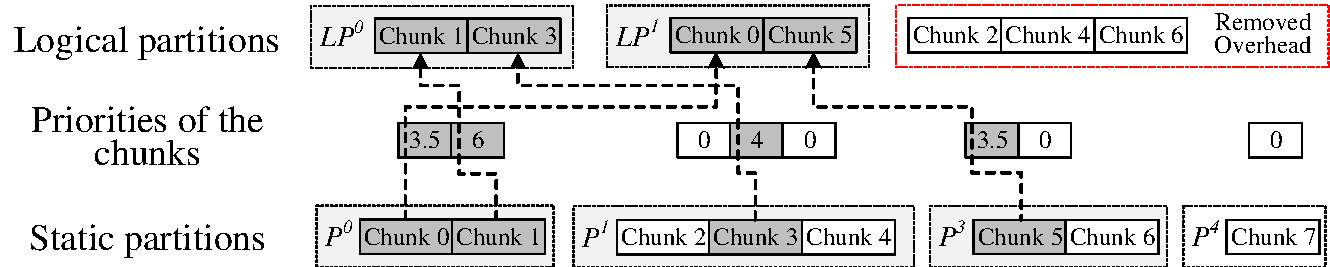
\includegraphics[width=3.5in]{repartition.pdf}
	\vspace{-22pt}
	\caption{Illustration of adaptive graph repartitioning, where \textit{chunk 0} and \textit{chunk 1} of $P^0$, \textit{chunk 3} of $P^1$, and \textit{chunk 5} of $P^2$ are active for concurrent jobs and the remaining chunks are inactive}
	\label{repartition}
	\vspace{-16pt}
\end{figure}

Because processing the graph data along various orders does not affect the accuracy of vertex values~\cite{Maiter,HotGraph,Wonderland}, the active chunks are judiciously loaded by GraphSO to construct the logical partitions, thereby enabling the loaded graph data to be shared by more jobs.
The key idea is to preferentially load the most-frequently-used chunks, i.e., the ones required by more jobs or owning more hub-vertices, to construct the logical partitions.
In this way, more chunks can be activated for concurrent jobs and most chunks in each loaded logical partition can be repeatedly accessed by more concurrent jobs, thus enabling higher utilization of each loaded logical partition.
To achieve this goal, a priority is assigned to each active chunk to schedule their loading order.
In essential, it is set by two rules. First, the chunk is assigned with the higher priority when it has more related jobs and more active vertices.
Second, the vertices of the chunk with the higher average degree need to be assigned with higher priorities.
Thus, the priority, e.g., $Pri(C_m)$, of each active chunk, e.g., $C_m$, can be determined by:
\vspace{-5pt}
\begin{equation}
\label{eq:priority}
	Pri(C_m) =  N(J_m) \cdot N(A_m) \cdot \frac{\sum_{v_i \in V_m} D(v_i)}{N(V_m)} ,
\end{equation}
where $V_m$ is the set of source vertices in $C_m$, $D_i(v_i)$ denotes the degree of vertex $v_i$, and $N(V_m)$ represents the number of source vertices in $C_m$.  $N(J_m)$ is the number of related jobs for $C_m$. $N(A_m)$ is the number of active vertices in $C_m$.
$N(V_m)$, $D(v_i)$ and the initial values of $N(A_m)$ and $N(J_m)$ can be obtained at preprocessing phase, while $N(A_m)$ and $N(J_m)$ are incrementally updated during the execution. Then, the loading order of the chunks can be scheduled according to their priorities.

After that, the active chunks are loaded and reassigned together by GraphSO to construct new logical partitions according to the procedure \textit{GenerateLogicalPartition}() in Algorithm~\ref{code3}, where the size of each logical partition needs to meet the requirement of the integrated graph processing system because the suitable size of partition (i.e., the static partition size $|P|$) is different for various systems.
Specifically, it first gets the suitable number of the active chunks based on their priorities to construct a logical partition $LP^i$ (Line~\ref{SortAID}).
Then, these chunks of $LP^i$ are sorted according to their chunk IDs, thereby providing an opportunity to exploit the sequential disk I/O (Line~\ref{SortID}).
If $LP^i$ has not loaded into the memory, a shared buffer (i.e., \textit{Buf}) is set up to store it (Lines~\ref{not}-\ref{create}), and the chunks of $LP^i$ are sequentially loaded into \textit{Buf} (Lines~\ref{load1}-\ref{load2}). Elsewise, $LP^i$ can be obtained in the shared memory (Line~\ref{attach}).
Finally, the $LP^i$ stored in \textit{Buf} is used as the returned results to be handled by the concurrent jobs (Line~\ref{returnLP}). Fig.~\ref{repartition} shows how to repartition the graph. We can observe that the I/O traffics associated with the chunks $chunk 2$, $chunk 4$, and $chunk 6$ can be removed by our repartitioning strategy.


\vspace{-6pt}
\subsubsection{Efficient Processing of Logical Partitions}\label{section:Scheduling}
\vspace{-2pt}

When a logical partition is generated and loaded, its related jobs are triggered to handle it, while the unrelated jobs will be suspended to wait for loading their active logical partitions. When the current logical partition has been processed by its related job, the next logical partition will be generated.
This procedure $Schedule$() is described in Algorithm~\ref{code3}.
In detail, when $Schedule$() is called by a job $j$, it first generates and loads a logical partition $LP^i$ by calling the procedure \textit{GenerateLogicalPartition}(), and then the related jobs (i.e., $J^i$) of $LP^i$ are obtained (Line~\ref{getjobs}).
The related jobs in \emph{suspended\_queue} are resumed to handle $LP^i$ (Line~\ref{resume}).
If $LP^i$ does not need to be handled by the current job $j$, the job $j$ will be suspended (Lines~\ref{suspend1}-\ref{suspend2}).
Then, it removes job $j$ from $J^i$ (Line~\ref{Remove}).
Finally, the logical partition $LP^i$ is provided as a return result to job $j$ for processing (Line~\ref{return}).

To efficiently stream the logical partitions into the LLC, the processing of their chunks need to be synchronized for different jobs. Only when a streamed chunk has been handled by its related jobs, the next chunk can be handled.
However, the computational load of a chunk is usually skewed for different jobs because of the heterogeneity in both the computational complexity and the number of active vertices in current chunk. The computational load of job $j$ for the processing of chunk $C_m$ can be gotten by $L_j(C_m) = \theta_j \cdot \sum_{v_i \in V_m \cap A_j}{N_m^+(v_i)}$, where $A_j$ is the active vertices set of the job $j$ in current iteration, $N_m^+(v_i)$ denotes the number of $v_i$'s outgoing edges in $C_m$, and $\theta_j$ is the profiled average execution time to process an edge in job $j$.
After that, it unevenly assigns the computing resources  to different jobs according to their calculated computational load. In this way, each chunk can be reused in the LLC by its related jobs, thereby reducing the data access cost.

\vspace{-6pt}
\subsection{Structure-aware Buffering for Concurrent Jobs}\label{section:Caching}
\vspace{-2pt}
In practice, the same graph data are usually repeatedly accessed by multiple concurrent jobs, because these jobs need to iteratively handle this graph iteration by iteration until convergence.
Besides, as shown in Fig.~\ref{active_ratio_times}(b), some graph data need to be accessed more frequently by these jobs.
Therefore, there is an opportunity to improve the performance of the concurrent jobs by effectively buffering the frequently-used graph data in the main memory.
%Although some existing solutions~\cite{G-store,FlashGraph,TurboGraph,Wonderland} have been proposed to buffer graph data in the main memory to reduce data access cost, the number of the related jobs associated with different chunks are usually skewed and also evolve with time. As a result, with existing solutions, the buffered graph data may only be needed by a few jobs, incurring the lower utilization of the buffered graph data.
Although many graph processing systems~\cite{G-store,FlashGraph,TurboGraph,Wonderland} have used the caching technique to reduce the I/O overhead, they still suffer from much redundant data storage and access cost when handling concurrent jobs. Specifically, the existing solutions~\cite{G-store,FlashGraph,TurboGraph,Wonderland} are designed to buffer the graph data in the main memory for each job separately, and multiple copies of the same graph data and also many graph data which are not important to multiple concurrent jobs will be buffered in the main memory when supporting the execution of multiple concurrent jobs.
These graph data cause serious contention for the main memory, which leads to significant data thrashing. Besides, the number of the related jobs associated with different chunks is usually skewed and varies over time. When using the existing solutions~\cite{G-store,FlashGraph,TurboGraph,Wonderland} to support the execution of multiple concurrent jobs, the buffered graph data may be needed by only a few jobs (or even one job). It eventually results in the low utilization of the buffered graph data.

%Besides, they buffer graph data for each single graph processing job separately. Thus, multiple copies of the same graph data are buffered in the main memory and these graph data also suffer from serious contention for the memory.
%much unnecessary and high data access overhead to the execution of concurrent jobs.

\begin{table}[!t]
	%\vspace{-12pt}
	\renewcommand{\arraystretch}{1.15}
	\caption{Proprieties of Graph Datasets}\label{T2}
	\vspace{-0.35cm}
	\centering
	\small
	\setlength{\tabcolsep}{1.3mm}{
		\begin{tabular}{l c c c}
			\hline
			Datasets & Vertices & Edges & Sizes\\
			\hline
			Twitter(TW)~\cite{LAW} & 41,652,230 & 1,468,365,182  & 17.5 GB\\
			Friendster(FS)~\cite{SNAP} & 65,608,366 & 1,806,067,135  & 22.7 GB\\
			Uk-2007(U7)~\cite{LAW} & 105,896,555 &
			3,738,733,648   & 46.2 GB\\
			Uk-union(UN)~\cite{LAW} & 133,633,040 & 5,507,679,822  & 68.3 GB\\
			Clueweb12(CW)~\cite{LAW} & 978,408,098 & 42,574,107,469 & 317 GB\\
			\hline
	\end{tabular}}
	\vspace{-12pt}
\end{table}

To address this challenge, we propose an efficient buffering strategy to judiciously buffer only one copy of the common chunks in a buffer (called buffer space) of the main memory to be shared by concurrent jobs, thereby enabling the buffered graph data to be reused by more jobs to further reduce data access cost. Specifically, the chunks with more related jobs and more active vertices need to be buffered in the buffer space because most proportion of the graph data in these chunks can be reused by more concurrent jobs.
Besides, the chunks with more hub-vertices need to be buffered in the buffer space because they need to be repeatedly loaded into the main memory.
%because the most-frequently-used chunks need to be frequently accessed by the concurrent jobs, these
Therefore, the most-frequently-used chunks (i.e., the ones with higher priority determined by the Formula~\eqref{eq:priority}) are tried to be preferentially cached in the buffer space.
In this way, the I/O traffic for loading these chunks can be efficiently spared by shielding the frequently-used graph data from thrashing and enabling the cached chunks to be effectively reused by more concurrent jobs, thereby minimizing the I/O cost.

%sparing more main memory resource to cache more graph data to further reduce data access cost for these jobs.

%buffer the graph data for the concurrent graph processing jobs. Specifically,

%Specifically, during the execution, the loading frequency of different chunks is usually skewed, and the chunks with many hub-vertices need to be repeatedly loaded into the main memory.
%These characteristics allows us to efficiently optimize the buffer management for the concurrent graph processing jobs in the following way.

%Because the chunks are synchronously streamed by GraphSO to serve the execution of the concurrent jobs, it allows us to propose an efficient buffering strategy to maintain only one copy of the common chunks in a buffer (called buffer space) of the main memory to be shared by concurrent jobs, sparing more main memory resource to cache more graph data to further reduce data access cost for these jobs.

%Besides,


To achieve this goal, we customize an insertion policy and an eviction policy to efficiently cache the chunks.
%we first order the chunks, e.g., $C_m$, according to expected loading frequency (i.e., $Pri(C_m)$).
%In theory, all hot-chunks should be cached. Thus, the region of buffer space size at the start of the ordered chunks is set as high-frequency range, and the remainder is labeled as low-frequency range. In fact, some chunks in the low-frequency range may also be repeatedly loaded by concurrent jobs, especially for large graphs. Therefore, we design a hybrid buffer management strategy to achieve preferential treatment to the chunks in high-frequency range while keeping flexibility in exploiting the reuse of other chunks.
%In detail,
%Specifically, each chunk cached in the memory is assigned with a \textit{Reuse Prediction State} (\textit{RPS}), which have two types of states: \textit{RS} and \textit{URS}.
%\textit{RS} is used to indicate that the corresponded chunks may be reused in the following iterations, and \textit{URS} is used to indicate that the corresponded chunks may not be reused in the following iterations.
Within each iteration, the active chunks are loaded into the memory and cached by the following strategies:
\vspace{-4pt}
\begin{itemize}
	\item \textit{Insertion Policy}: When the buffer space is not full and the loaded chunks have not cached, these chunks need to be inserted into buffer space.
	%If the loaded chunks are in the high-frequency range (indicating these chunks may need to be reused by the jobs in the following iterations), their \textit{RPS}s are set as \textit{RS}.
	%If the loaded chunks in the high-frequency range, their \textit{RPS}s are set as \textit{RS}. The \textit{RPS}s of the rest chunks are set as \textit{URS}.
	%\item \textit{Hit-promotion Policy}: If the loaded chunks have been cached in the main memory, it indicates that these chunks may be reused in the next iteration. Thus, the \textit{RPS}s of these chunks are set as \textit{RS}.
	\item \textit{Eviction Policy}: If the buffer space is full and the loaded chunk have not been cached yet, the cached chunk, e.g., $C_m$, with the lowest priority, e.g., $Pri(C_m)$, will be evicted.
	%If the states of all cached chunks are \textit{RS}, the chunk with $AD$ value lower than that of loaded chunk is replaced.
	%\item \textit{Demotion Policy}: If the cached chunks are not handled by concurrent jobs in the current iteration (indicating these chunks may have already been converged and do not need to be handled by concurrent jobs in the next iteration any more), their \textit{RPS}s are set as \textit{URS} after this iteration.
\end{itemize}
\vspace{-4pt}

By this way, the memory resources are fully utilized and the I/O traffic is further reduced by reusing the cached chunks in the main memory.

\begin{figure*}[t]
	%\vspace{-0.5cm}
	\begin{minipage}[t]{0.32\linewidth}
		\centering
		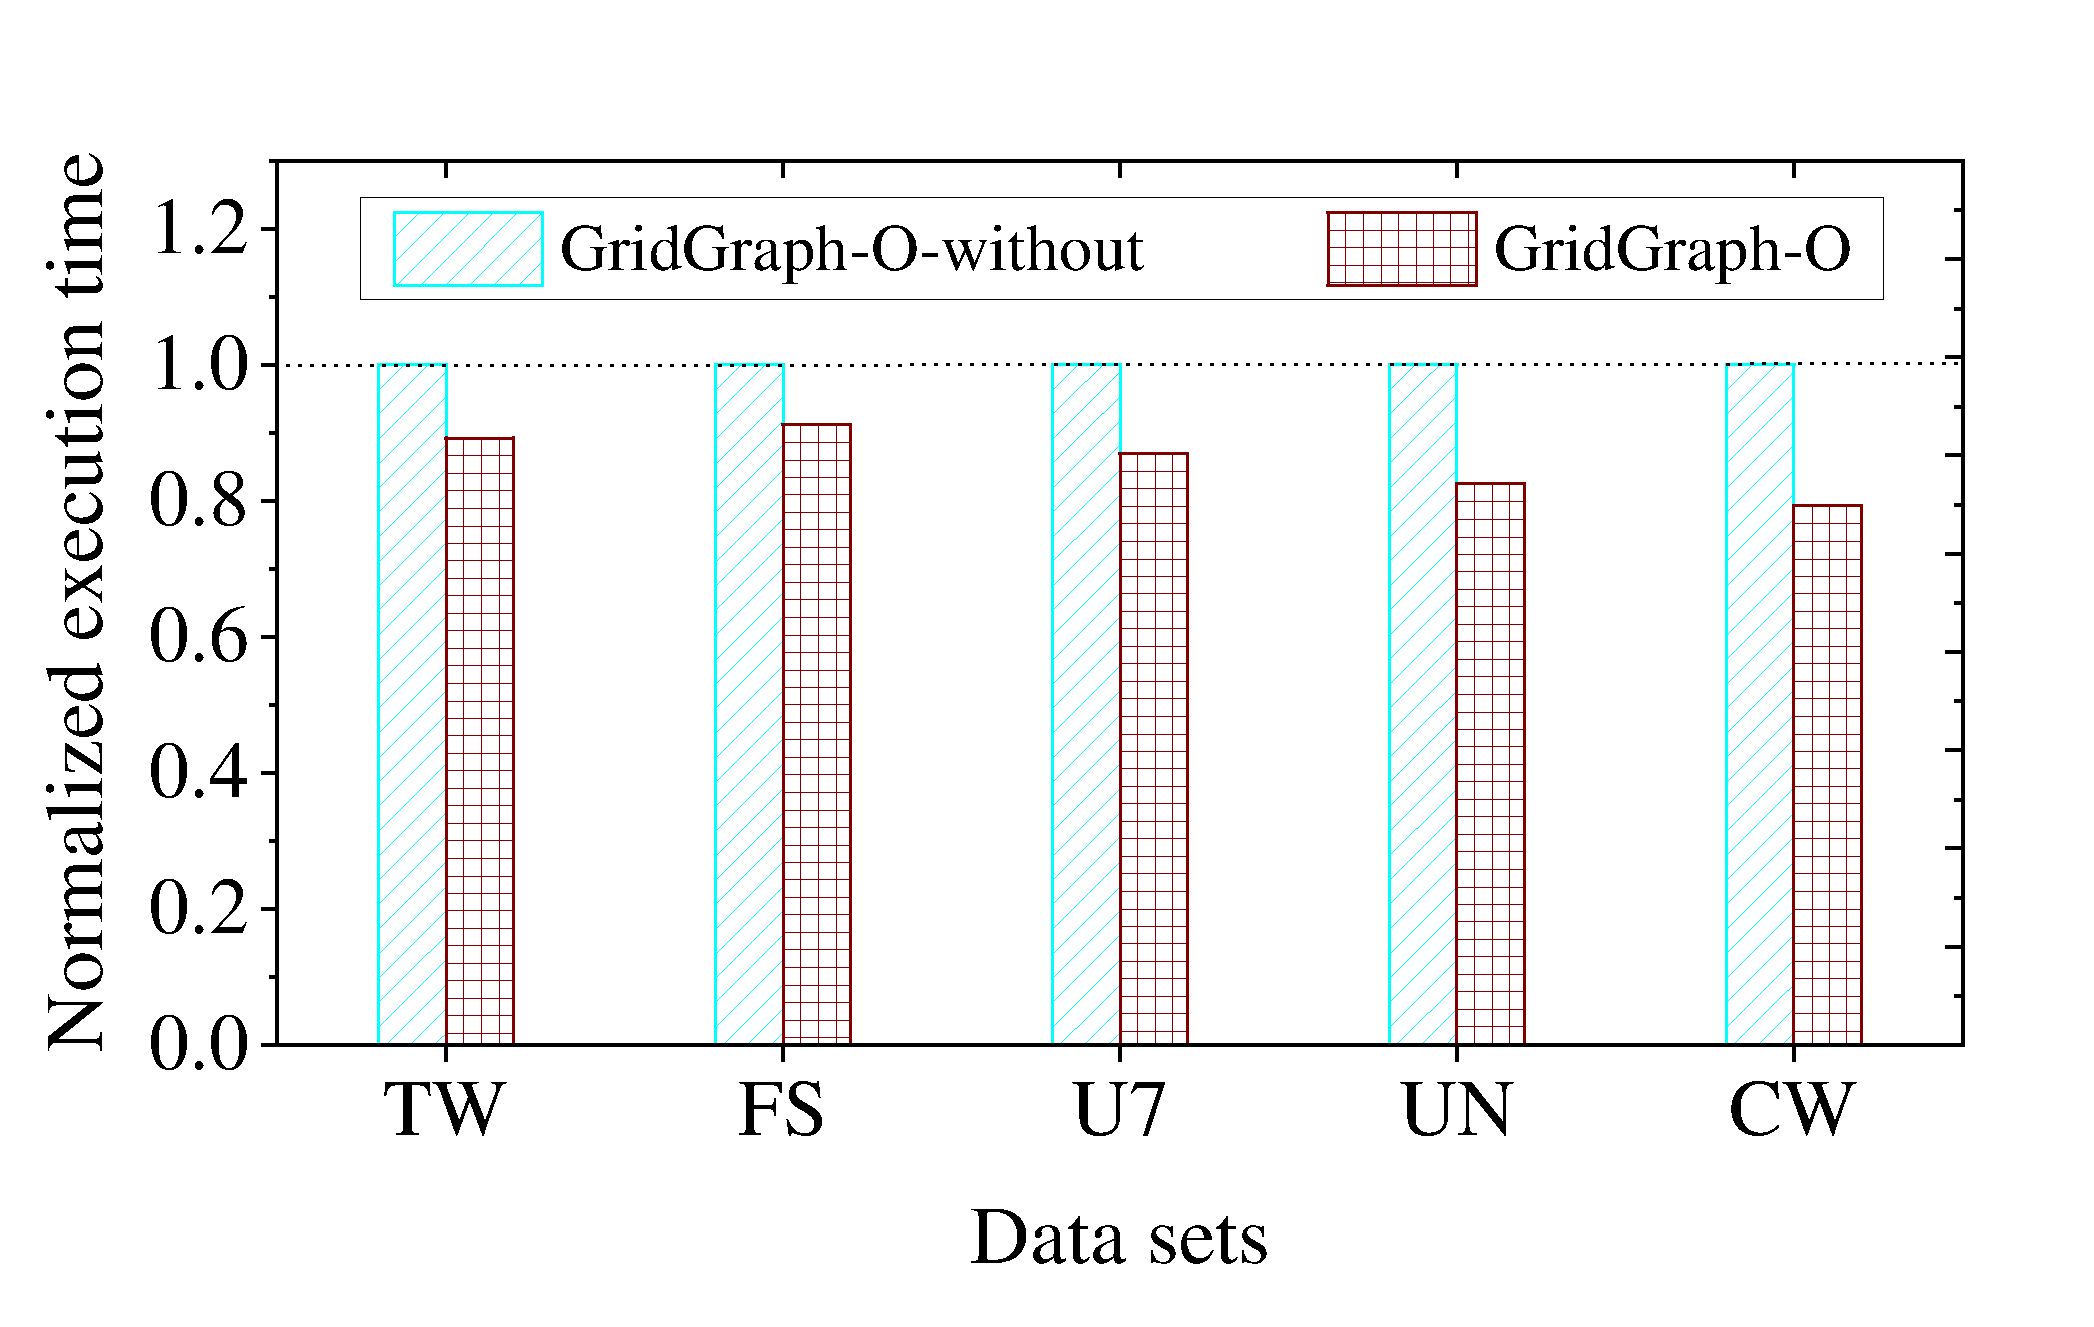
\includegraphics[width=6cm]{schedule.pdf}
		\vspace{-0.95cm}
		\caption{Execution time for the four jobs without/with our structure-aware buffering strategy}
		\label{schedule}
	\end{minipage}
	\hfill
	\begin{minipage}[t]{0.32\linewidth}
		\centering
		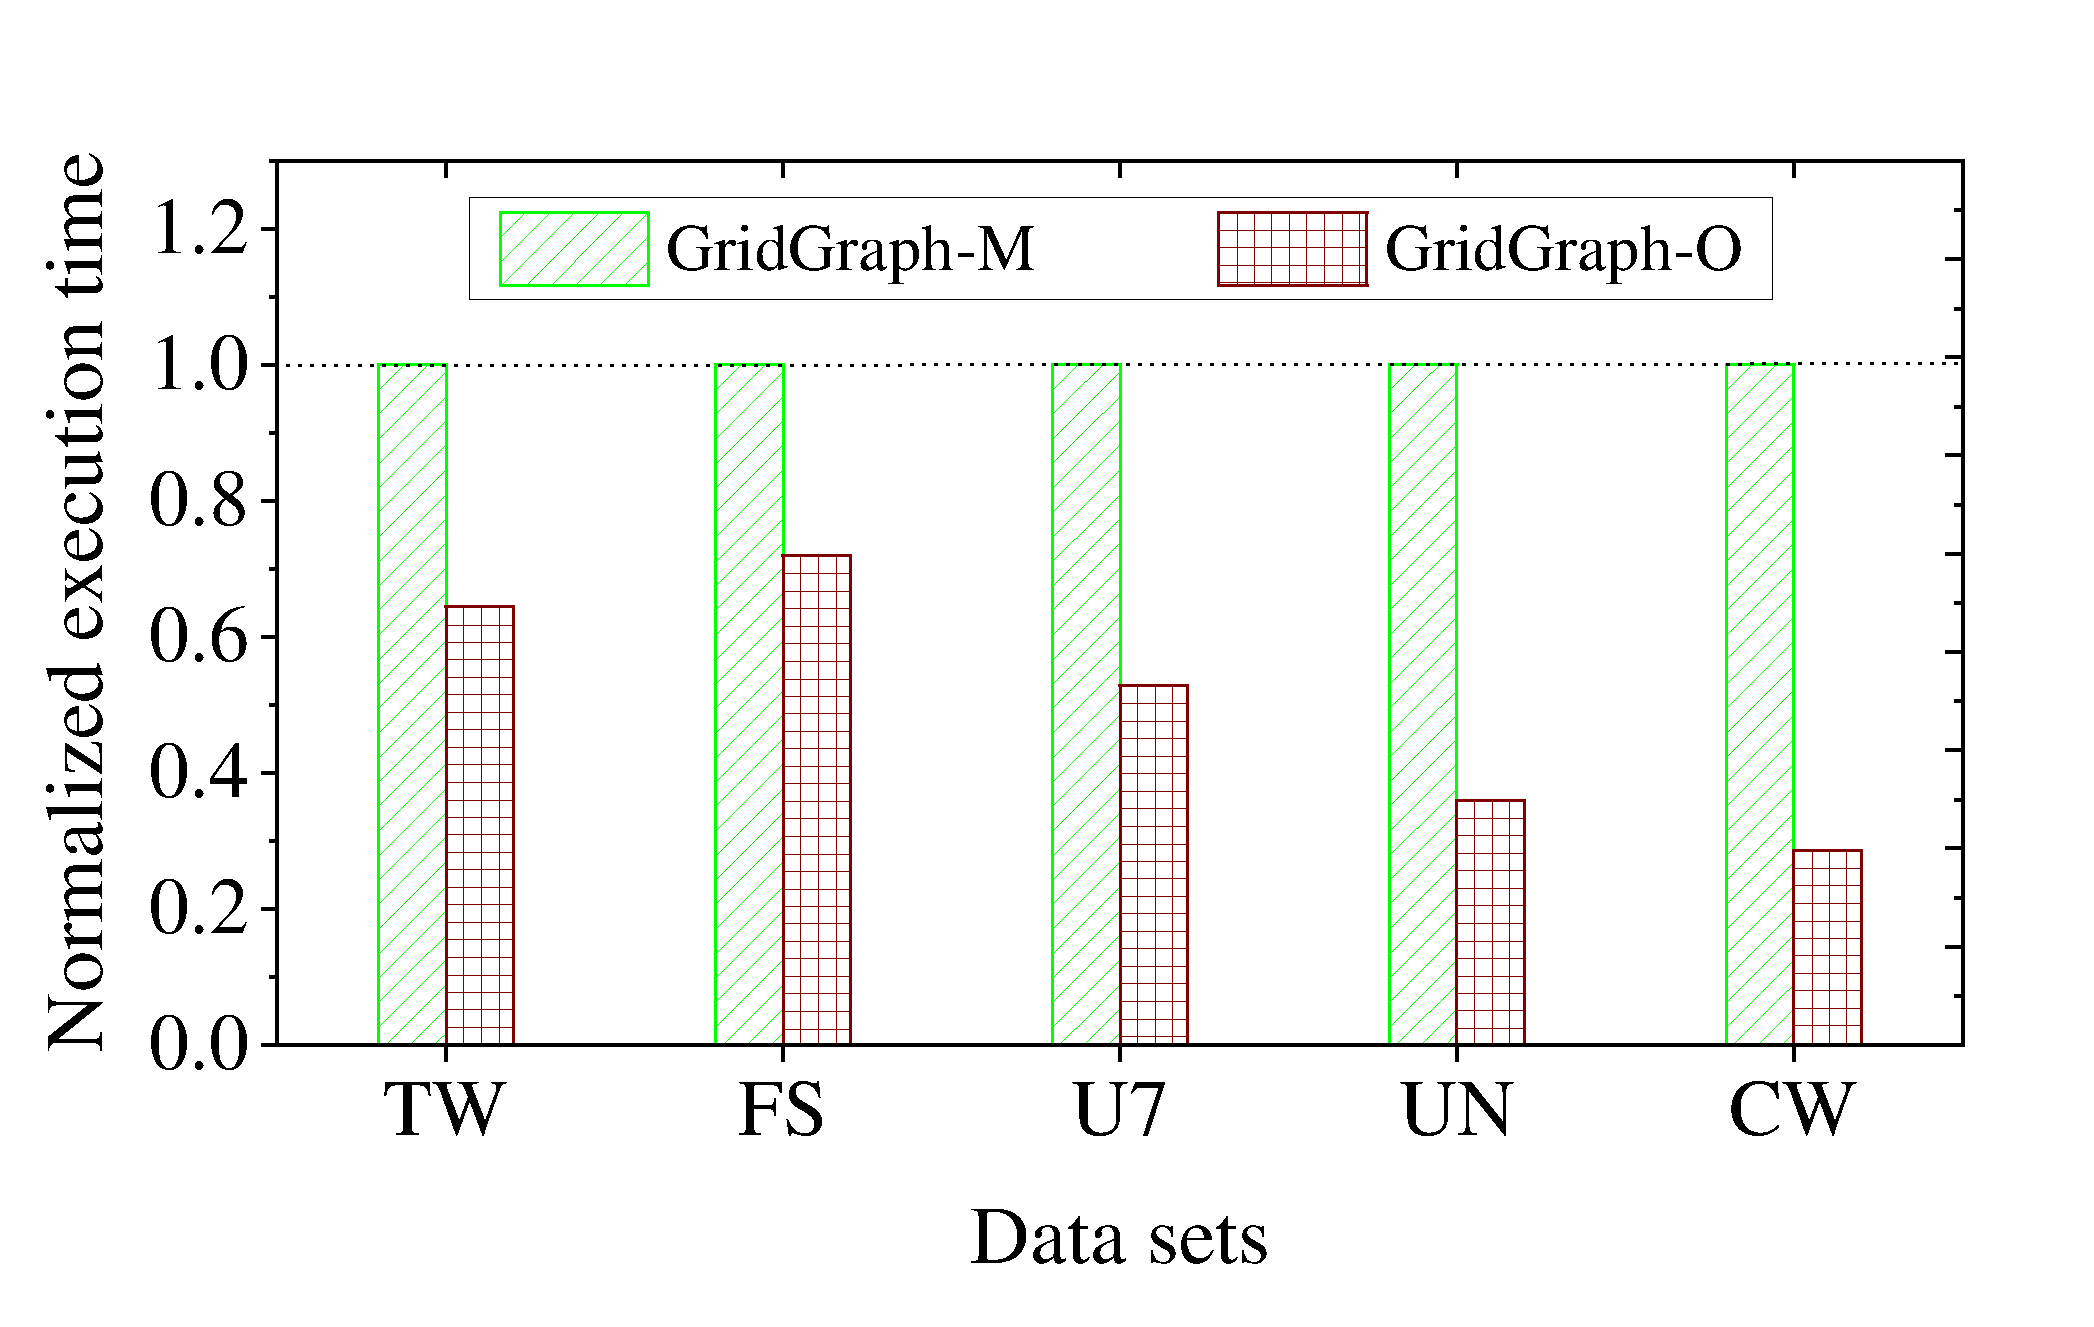
\includegraphics[width=6cm]{exe_time.pdf}
		\vspace{-0.95cm}
		\caption{Comparison of execution time for running the four jobs on various schemes}
		\label{exe_time}
	\end{minipage}
	\hfill
	\begin{minipage}[t]{0.32\linewidth}
		\centering
		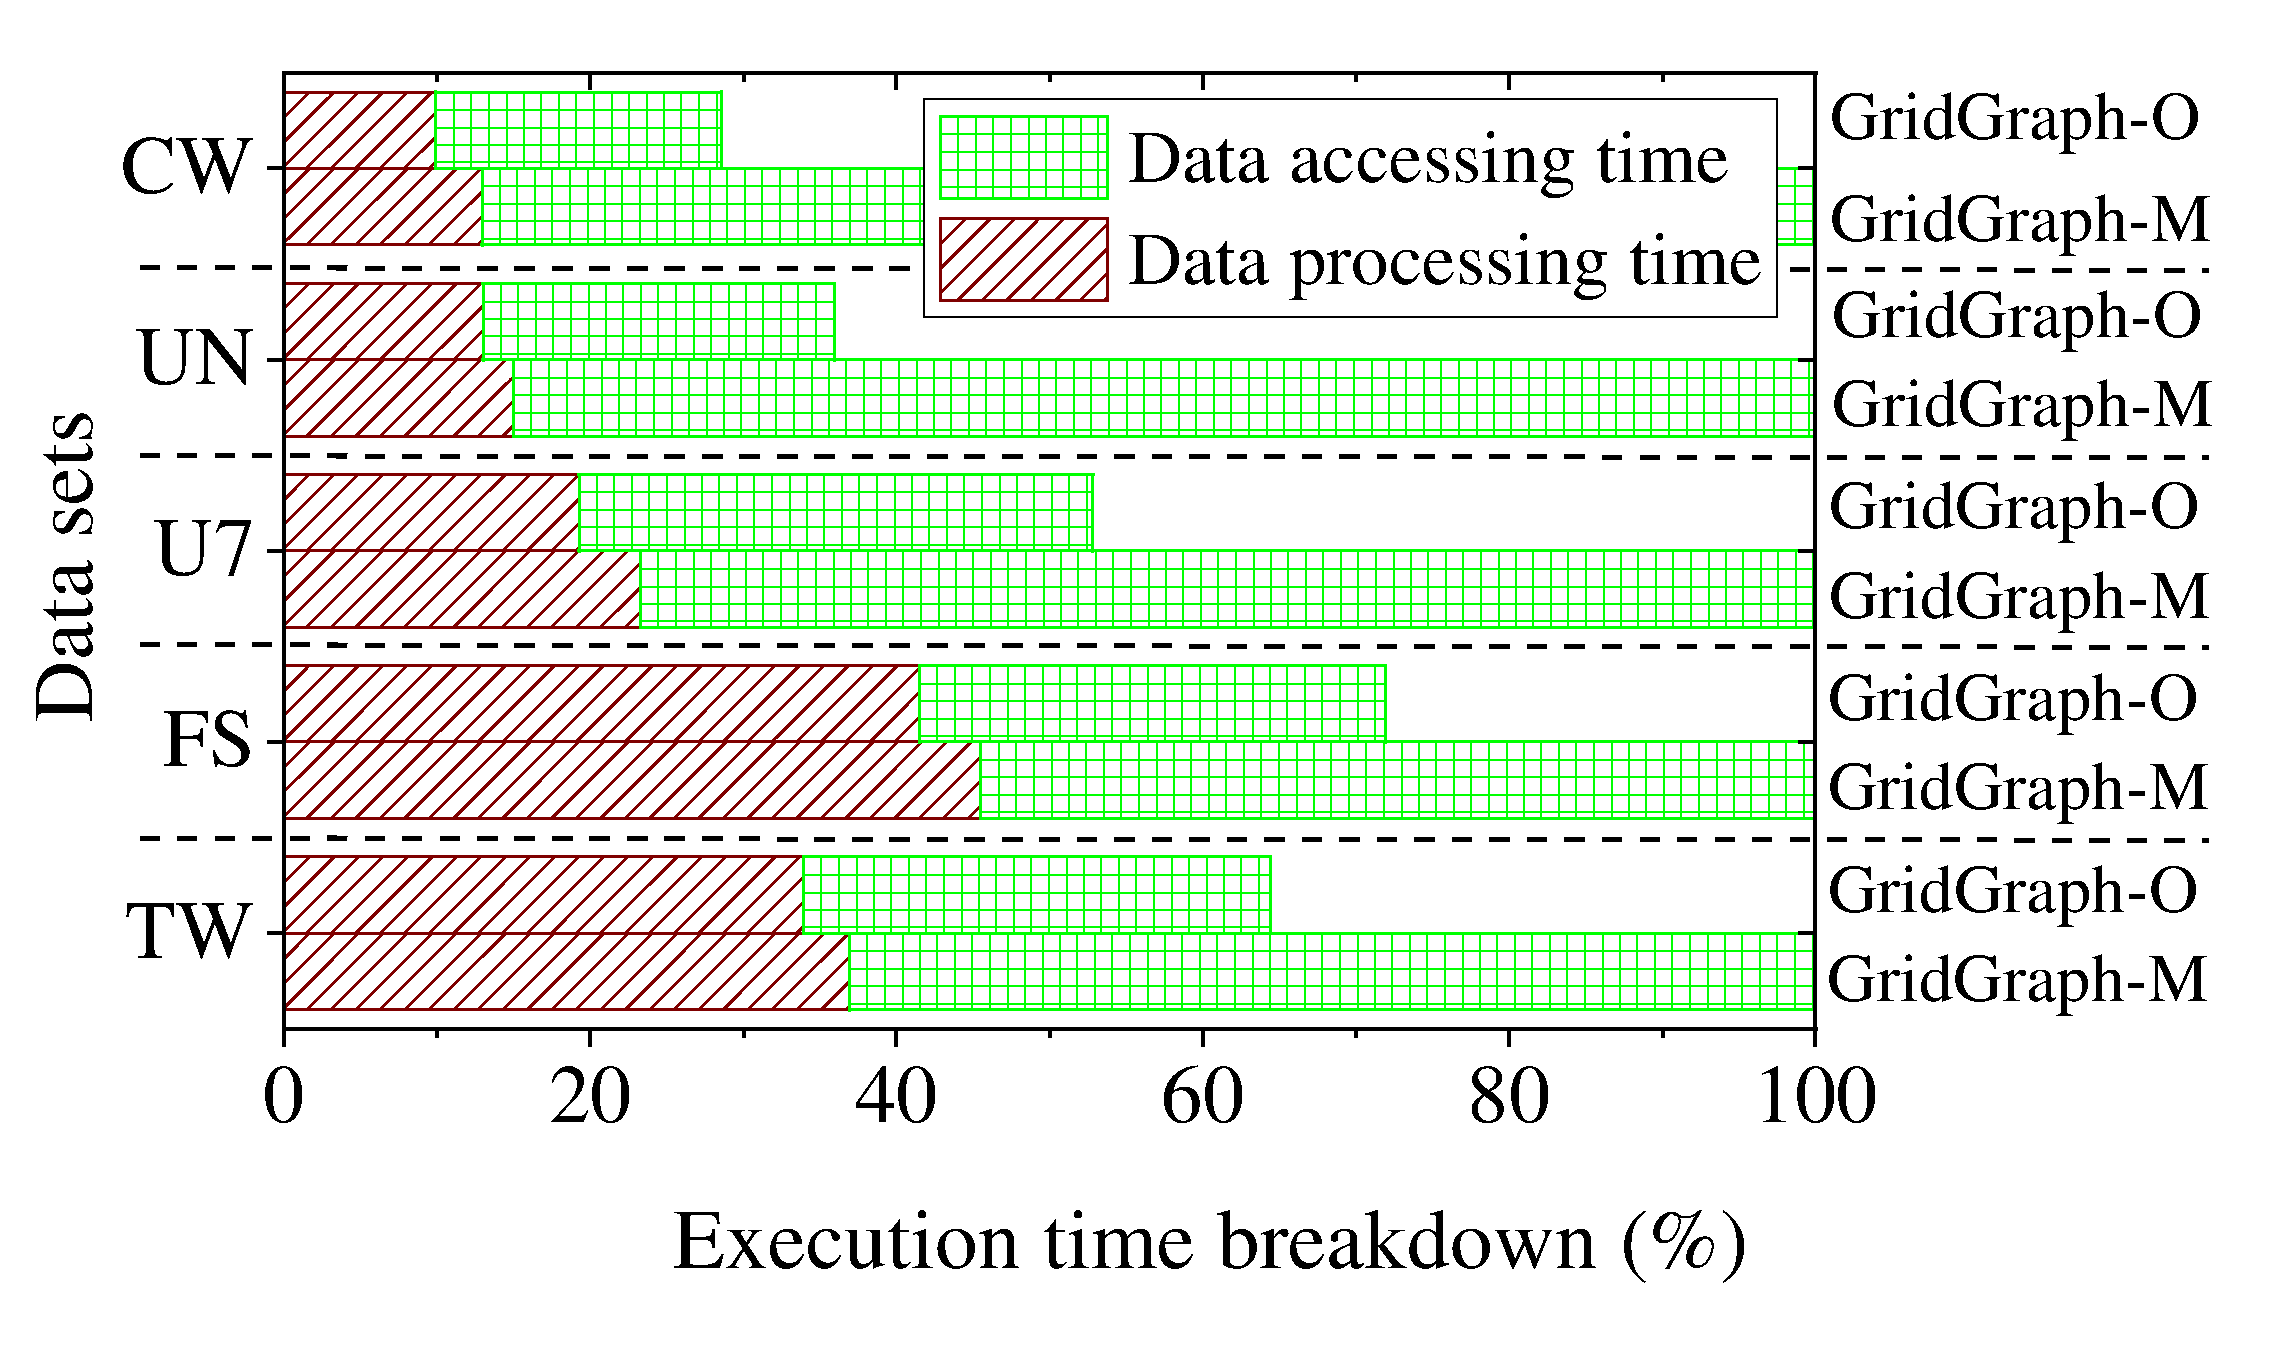
\includegraphics[width=6cm]{breakdown.pdf}
		\vspace{-0.95cm}
		\caption{Execution time breakdown of the four jobs on various schemes}
		\label{breakdown}
	\end{minipage}
	\vspace{-0.6cm}
\end{figure*}

\vspace{-8pt}
\section{Evaluation}\label{section:Evaluation}
%This section presents experimental evaluation of GraphSO in comparison with state-of-the-art solutions.

\vspace{-2pt}
\subsection{Experiment Setup}\label{section:4.1}
\vspace{-2pt}
The hardware platform adopted in the experiments is a single machine, which contains two Intel Xeon E5-2670 CPUs (each CPU owns 8 cores and 20 MB LLC), a 32 GB main memory and a standard 1 TB hard drive, running Linux kernel 2.6.32. All programs are compiled with gcc version 4.9.4 and cmake version 3.11.0. The datasets used in our experiments are five real-world graphs as detailed in Table~\ref{T2}, where their edge weights are generated randomly from the range [0, 256].
The benchmarks employ four popular graph processing algorithms, which containing: PageRank~\cite{PageRank}, Breadth-First Search (BFS)~\cite{BFS}, Single Source Shortest Path (SSSP)~\cite{SSSP}, and Weakly Connected Component (WCC)~\cite{SCC}.
These algorithms can be classified into two categories: \textit{all-active algorithm} and \textit{non-all-active algorithm}. Specifically, the former (e.g., PageRank and WCC) traverses the graph starting from all vertices at the beginning, whereas the latter (e.g., SSSP and BFS) starts from a subset of vertices at the beginning. Note that, in the real trace of Fig.~\ref{number_jobs}, the proportion of the former is about 34.2\%, and that of the latter is 65.8\%.
%, Belief Propagation (BP)~\cite{BP}, Alternating Least Squares (ALS)~\cite{ALS}, Random Walk (RW)~\cite{RW}, and Maximal Independent Set (MIS)~\cite{MIS}.
In our experiments, we simultaneously submit these algorithms to generate a specified number of jobs, where SSSP and BFS are submitted with the randomly selected starting vertices. The ratio of physical memory (i.e., available memory resource) used to cache graph data is set as 25\% by default. The chunk size $|C|$ is determined by the Formula~\eqref{eq:chunksize}. For example, $|C| \le 1.4$ MB for $FS$ with 8 MB reserved space size, thus $|C|$ is set to 1 MB by GraphSO.

To evaluate the performance of GraphSO, we integrate it into seven popular systems, i.e., GridGraph~\cite{GridGraph}, GraphChi~\cite{GraphChi}, X-Stream~\cite{X-stream}, DynamicShards~\cite{Vora}, LUMOS~\cite{LUMOS}, Graphene~\cite{Graphene}, and Wonderland~\cite{Wonderland}. In our experiments, we mainly show the performance improvement when GraphSO is integrated into GridGraph because it is the one of the state-of-the-art and the most popular graph processing systems~\cite{LUMOS, Wonderland}. We tersely discuss the results when integrating with the other systems in Section~\ref{section:Others}.
Specifically, GridGraph integrated with GraphSO (called GridGraph-O in our experiments) is also compared with another scheme, i.e., GridGraph-M~\cite{GraphM} (GridGraph integrated with GraphM). GraphM is the state-of-the-art graph storage system that allows the same graph data to be shared by the concurrent jobs on existing graph processing system.
Note that the experiments are also conducted in the same way for GraphChi, X-Stream, DynamicShards, LUMOS, Graphene, and Wonderland in Section~\ref{section:Others}. Note that Graphene performs on eight Samsung NVMe 950 Pro 512GB SSDs. Besides, we also evaluate the performance of CGraph~\cite{CGraph} to further demonstrate the efficiency of GraphSO.
All experiments are conducted for ten times and the reported results are the average value.


We use DynamicShards and LUMOS to illustrate how to integrate GraphSO with existing graph processing systems.
For DynamicShards, we insert \textit{GetActiveChunks}() and \textit{Schedule}() between successive iterations in the program to replace its repartitioning logic and the original graph load logic to achieve the lower repartitioning cost and the higher utilization of the loaded graph data. For LUMOS, we use the \textit{GetActiveChunks}() and \textit{Schedule}() to repartition its primary layout partitions and efficiently load the graph structure data for concurrent jobs.


%GraphSO can also be integrated with both DynamicShards and LUMOS.


\vspace{-8pt}
\subsection{Preprocessing Cost}
\vspace{-2pt}
Table~\ref{Preprocessing-table} depicts the preprocessing time of GridGraph, GraphChi, X-Stream, DynamicShards, LUMOS, Graphene, and Wonderland after integrating with GraphM and GraphSO, respectively.
We can find that little additional time is required by GridGraph-O, GraphChi-O, X-Stream-O, DynamicShards-O, LUMOS-O, Graphene-O, and Wonderland-O, to generate the \textit{TChunk} compared with GridGraph-M, GraphChi-M, X-Stream-M, DynamicShards-M, LUMOS-M, Graphene-M, and Wonderland-M, because GraphSO needs to collect little more information than GraphM.
For example, the additional time of GridGraph-O is about 5\%, 7.2\%, 6.5\%, 4.2\%, and 5.7\% for TW, FS, U7, UN, and CW, respectively. The extra storage cost required by GridGraph-O is also small and occupies 16.5\% (2.89 GB), 8.6\% (1.95 GB), 10.2\% (4.71 GB),  9.1\% (6.22 GB), and 7.8\% (24.73 GB) of the total storage overhead of TW, FS, U7, UN, and CW, respectively. Although GraphSO requires little extra overhead, much unnecessary I/O traffic can be reduced by it, as will be shown later.

\begin{table}[!t]
	\renewcommand{\arraystretch}{1.1}
	\caption{Preprocessing time (in seconds)}\label{Preprocessing-table}
	\vspace{-12pt}
	\label{T3}
	\small
	\centering
	\setlength{\tabcolsep}{0.8mm}{
		\begin{tabular}{c c c c c c}
			\hline
			& TW & FS & U7  & UN & CW \\
			\hline
			GridGraph-M & 463.7 & 716.6 & 1,803.4 & 2,681.1 & 22,401.9   \\
			GridGraph-O & 486.8 & 768.2 & 1,920.7 & 2,793.6 & 23,674.3  \\
			\hline
			GraphChi-M & 975.3 & 2,579.2 & 3,755.9 & 5,715.9 & 26,866.3  \\
			GraphChi-O & 1,052.4 & 2,814.5 & 3,922.5 & 6,145.8 & 28,013.8 \\
			\hline
			X-Stream-M & 252.3 & 462.2 & 927.8 & 1,254.2 & 9,891.3 \\
			X-Stream-O & 296.3 & 506.3 & 1,185.2 & 1,427.4 & 11,265.7  \\
			\hline			
			DynamicShards-M & 1,034.6 & 2,475.4 & 3,472.8 & 5,125.2 & 27,013.7  \\
			DynamicShards-O & 1,146.8 & 2,591.2 & 3,615.4 & 5,517.3 & 28,916.5 \\
			\hline			
			LUMOS-M & 579.6 & 945.9 & 2,406.7 & 3,780.4 & 27,930.8 \\
			LUMOS-O & 602.3  & 995.7 & 2,568.4 & 3,992.7 & 29,735.1 \\
			\hline
			Graphene-M & 8.2 & 11.3 & 116.2 & 242.7 & 617.5  \\
			Graphene-O & 9.1 & 12.8 & 127.6 & 258.3 & 651.9  \\
			\hline						
			Wonderland-M & 505.4 & 804.1 & 2,146.1 & 3,244.1 & 27,554.3 \\
			Wonderland-O & 528.5  & 855.6 & 2,263.3 & 3,356.6 & 28,826.7 \\
			\hline
	\end{tabular}}
	\vspace{-12pt}
\end{table}

\begin{figure*}[t]
	%\vspace{-0.4cm}
	\begin{minipage}[t]{0.31\textwidth}
		\centering
		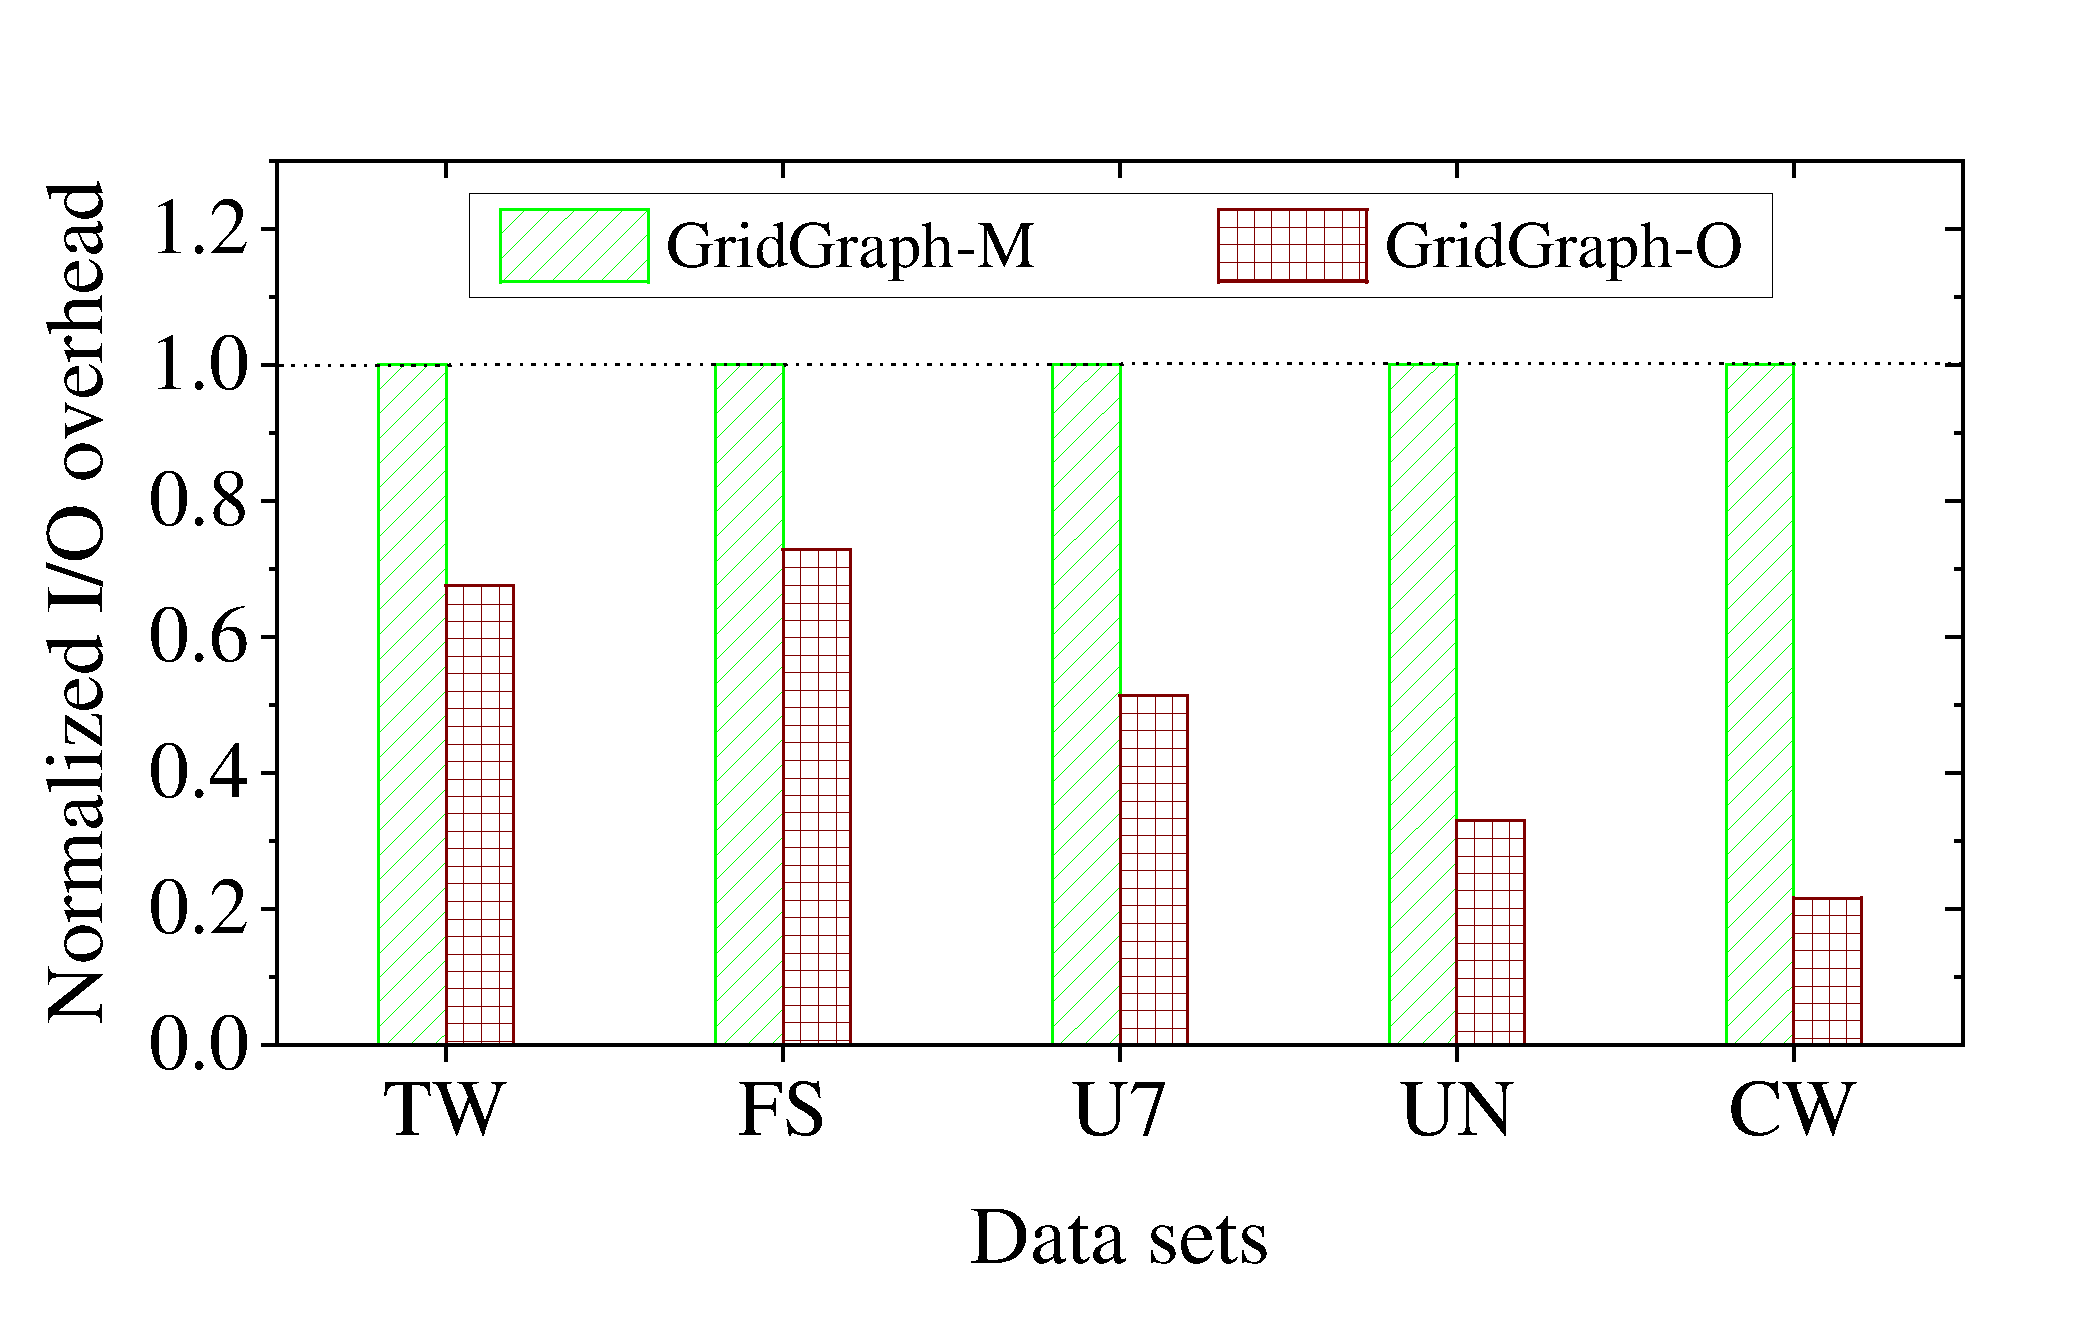
\includegraphics[width=6cm]{IO.pdf}
		\vspace{-0.98cm}
		\caption{Normalized I/O traffic for the four jobs on various schemes}
		\label{IO}
	\end{minipage}
	\hfill
	\begin{minipage}[t]{0.31\textwidth}
		\centering
		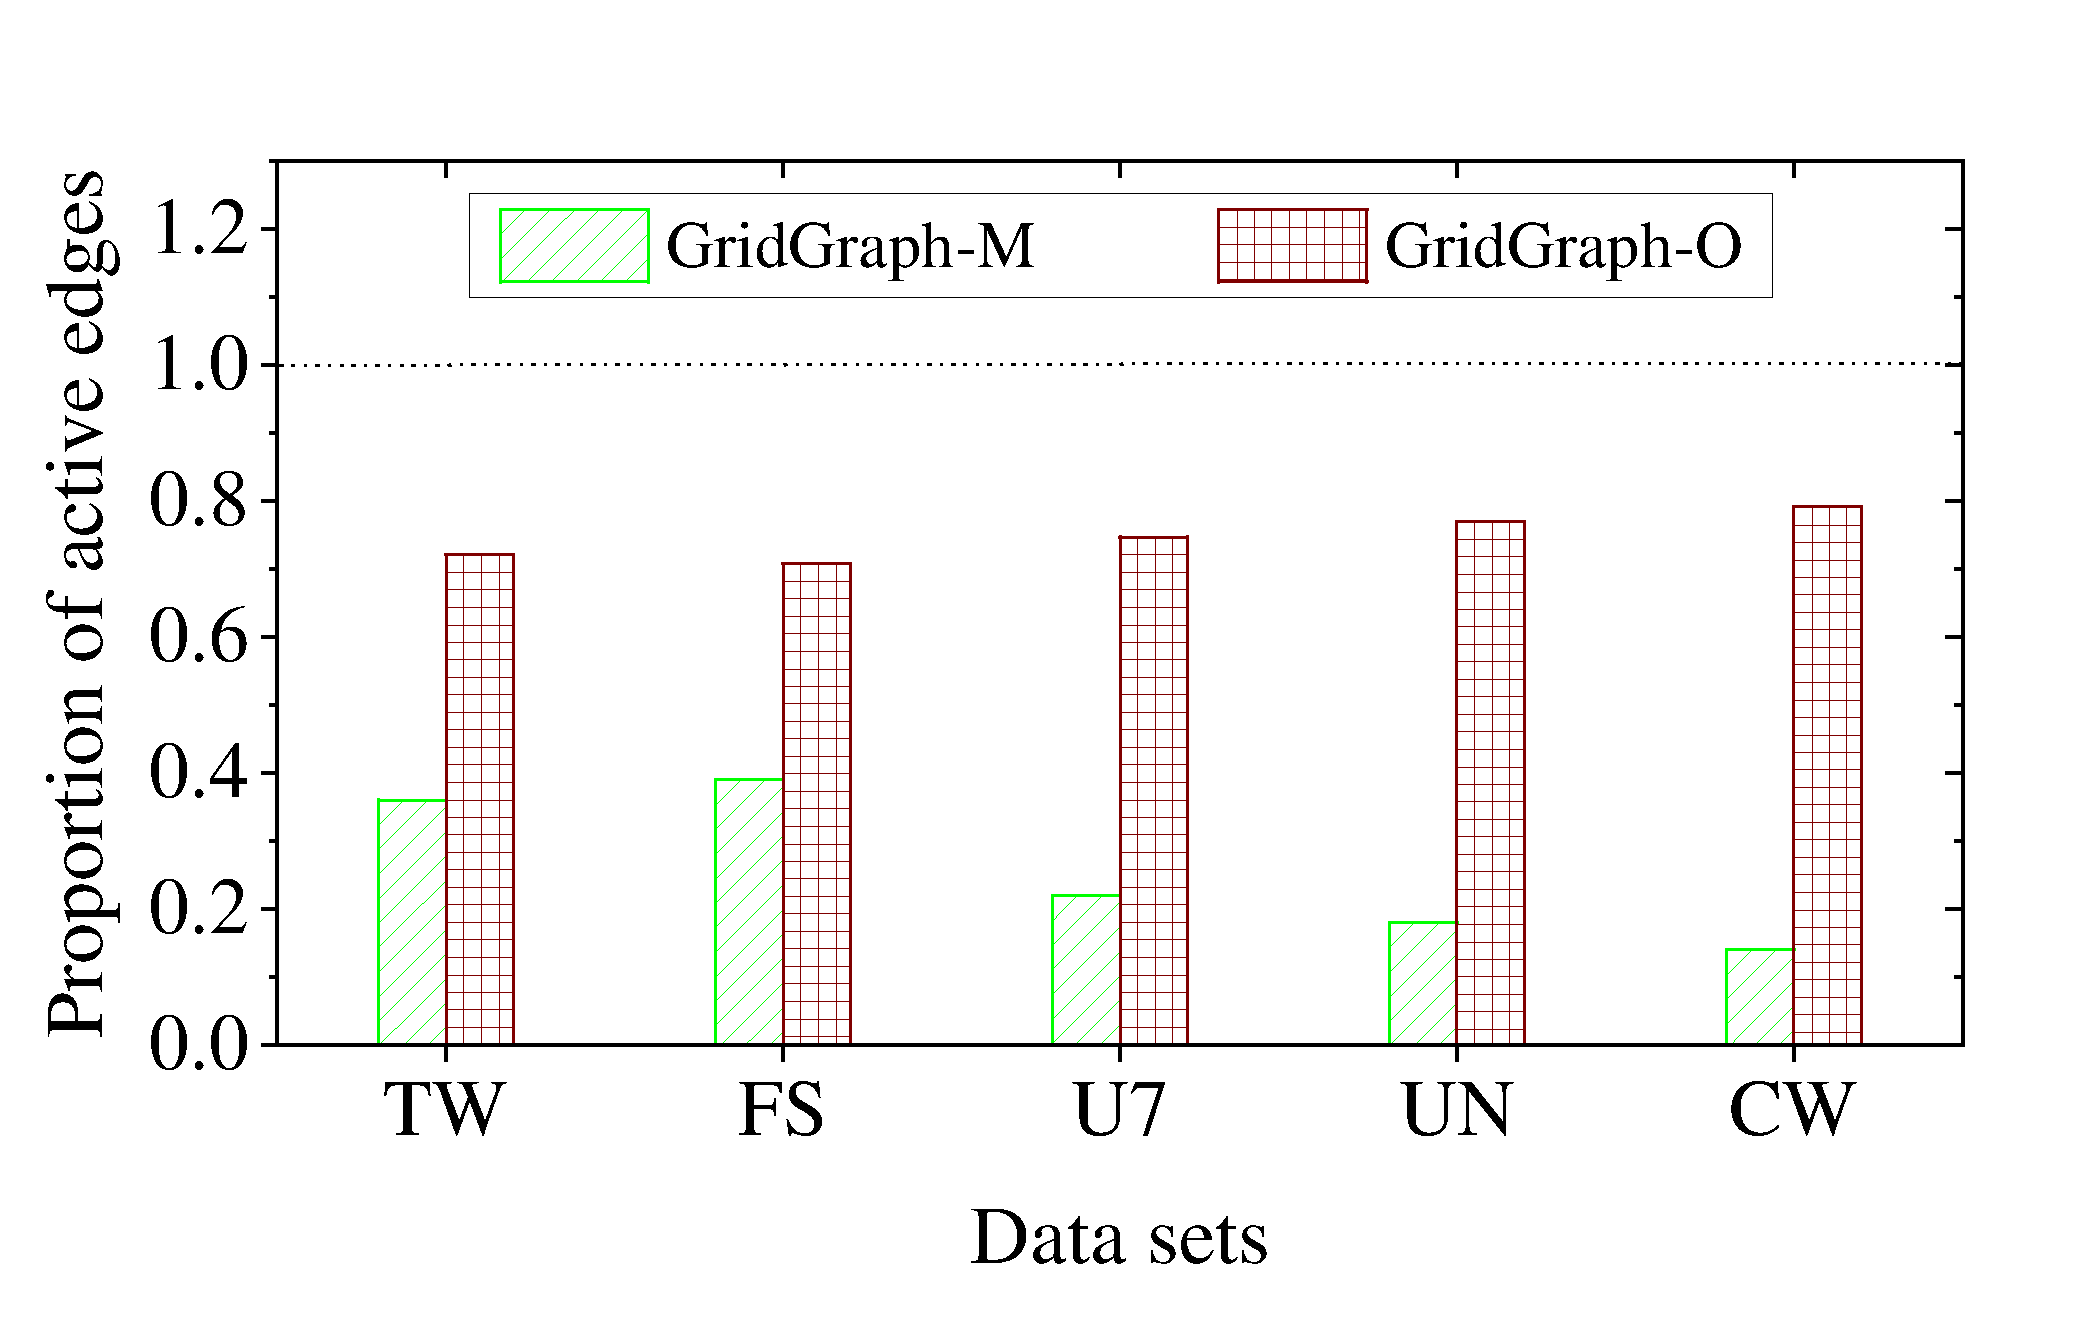
\includegraphics[width=6cm]{ratio_active.pdf}
		\vspace{-0.98cm}
		\caption{Proportion of the number of active edges to that of the total loaded edges}
		\label{ratio_active}
	\end{minipage}
	\hfill
	\begin{minipage}[t]{0.32\textwidth}
		\centering
		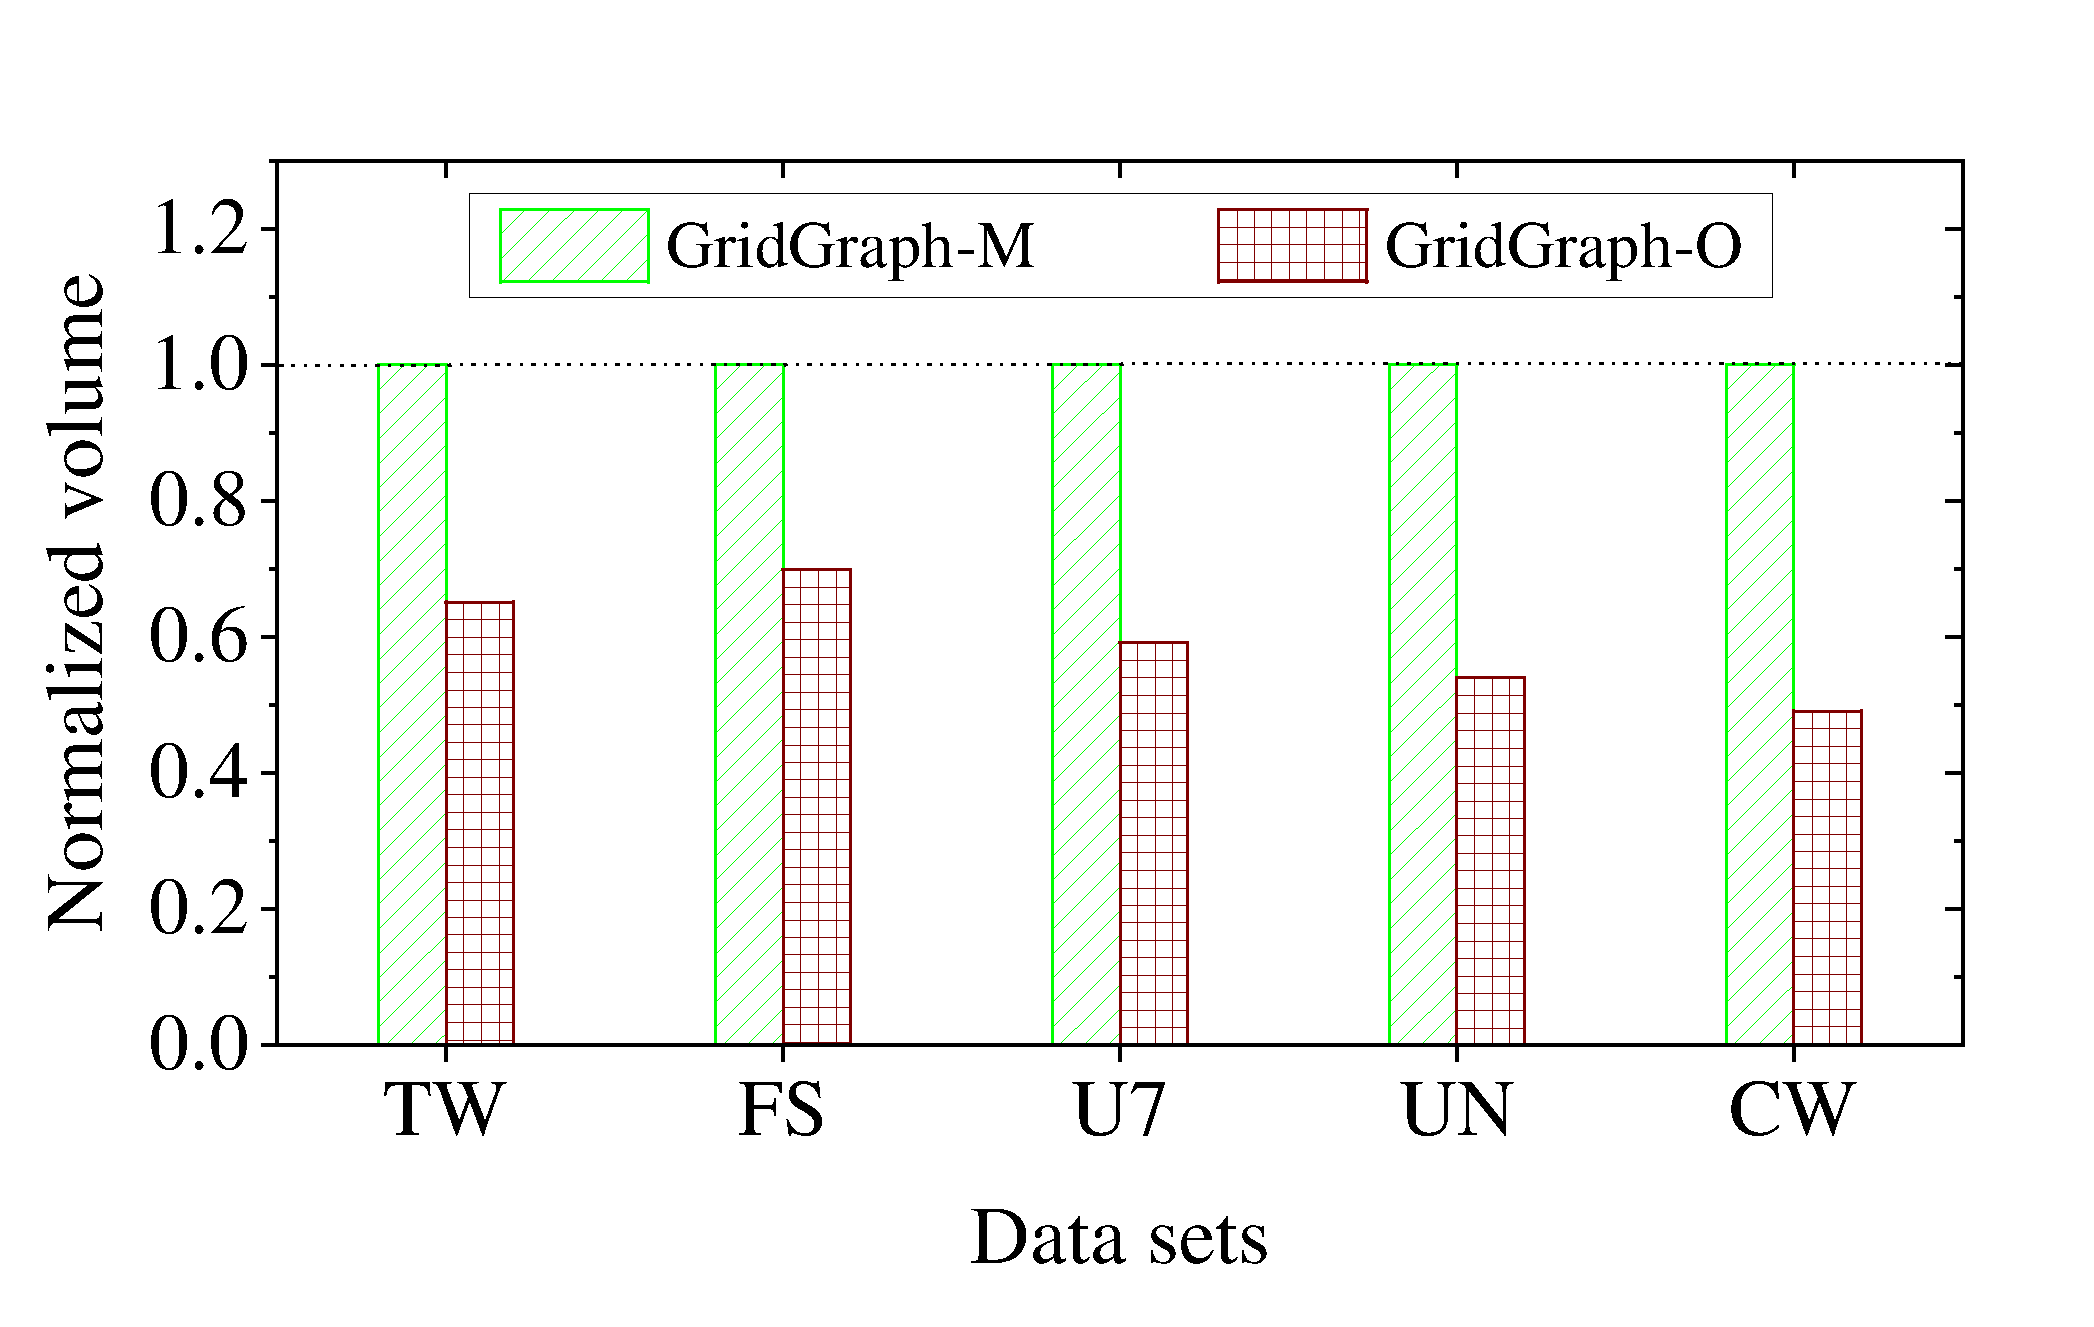
\includegraphics[width=6cm]{cache_swap.pdf}
		\vspace{-0.98cm}
		\caption{Volume of the graph data steamed into the LLC for the four jobs with various schemes}
		\label{cache_swap}
	\end{minipage}
	\vspace{-0.77cm}
\end{figure*}

\vspace{-8pt}
\subsection{Performance of Structure-aware Buffering Strategy}\label{section:4.3}
\vspace{-2pt}
First, we analyze the optimizations designed in GraphSO. All four algorithms (i.e., SSSP, PageRank, BFS, and WCC) are simultaneously submitted to generate four concurrent jobs, and then trace the execution time of concurrent jobs with/without our proposed optimization. Fig.~\ref{schedule} depicts the results.
GridGraph-O and GridGraph-O-without are the version of GridGraph-O with and without our structure-aware buffering strategy (Section~\ref{section:Caching}).
%only using the structure-aware adaptive graph repartitioning approach (Section~\ref{section:Repartitioning}), while the other optimizations are disabled. %GridGraph-O-WS is the version that further enables the structure-aware scheduling scheme (Section~\ref{section:Scheduling}) based on GridGraph-O-w/o, while
%GridGraph-O-WM is the version that further enables the   based on GridGraph-O-w/o.
We can find that
%GridGraph-O-WS requires shorter execution time than GridGraph-O-w/o because the loaded logical partitions are shared by more concurrent jobs.
GridGraph-O obtains better performance than GridGraph-O-without because the I/O overhead of the buffered chunks is eliminated for concurrent jobs.
For example, over CW dataset, the execution time of GridGraph-O is only 79.3\% of GridGraph-O-without.
Note that, for TW, FS, U7, UN, and CW, the execution time of the  GridGraph-O-w/o is 213, 298, 962, 1,012, and 9,909 seconds, respectively.

%\begin{figure*}[t]
%	\begin{minipage}[t]{0.31\textwidth}
%		\centering
%		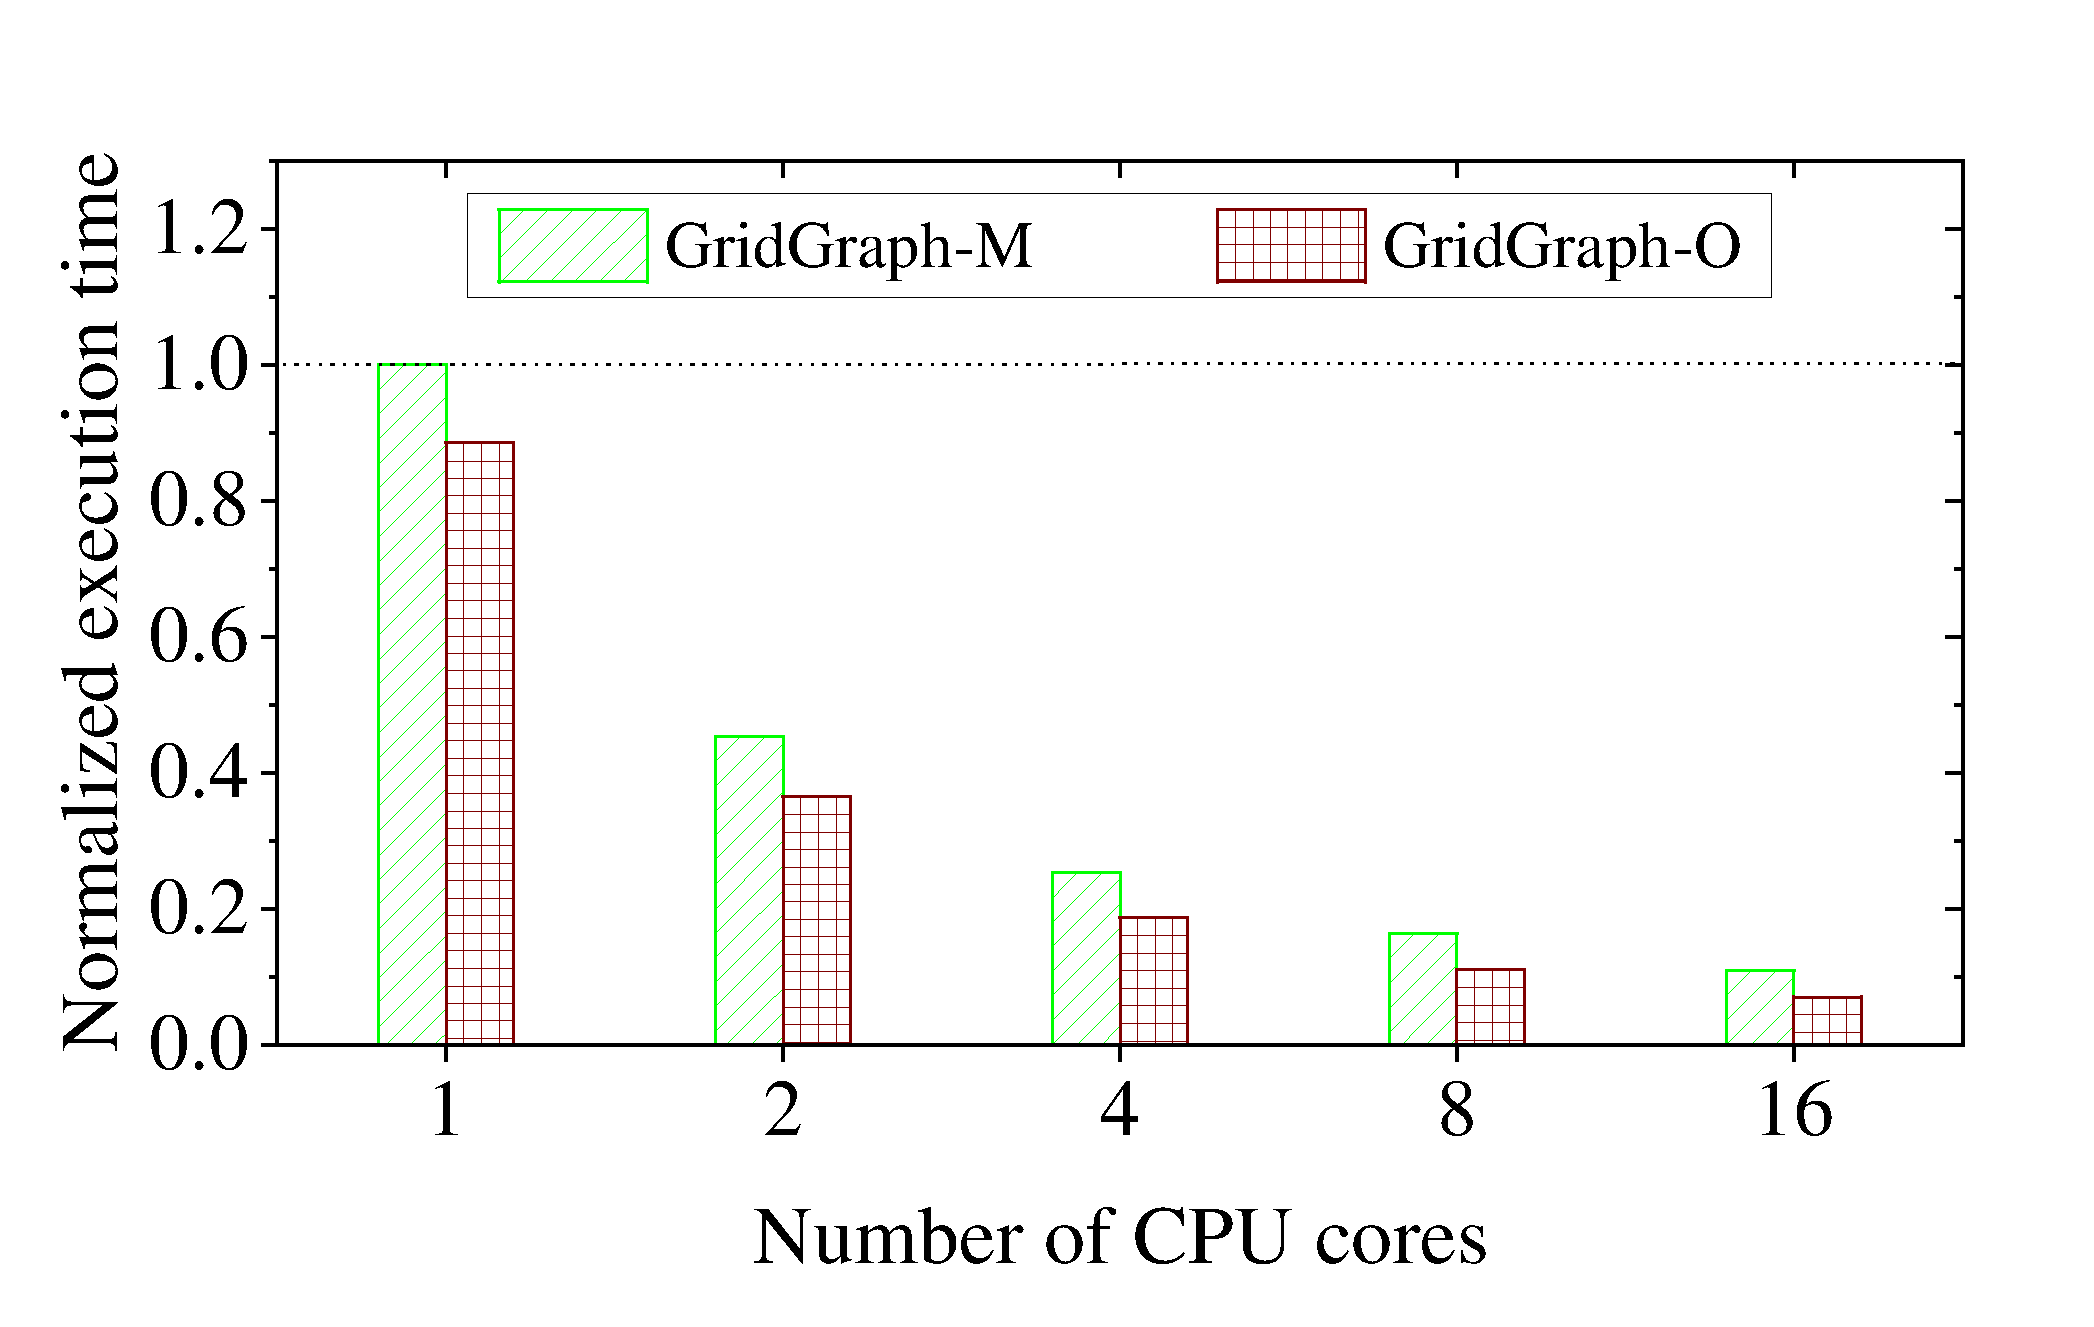
\includegraphics[width=6cm]{Scal_workers.pdf}
%		\vspace{-0.98cm}
%		\caption{Total execution time for different number of CPU cores}
%		\label{Scal_workers}
%	\end{minipage}
%	\hfill
%	\begin{minipage}[t]{0.31\textwidth}
%		\centering
%		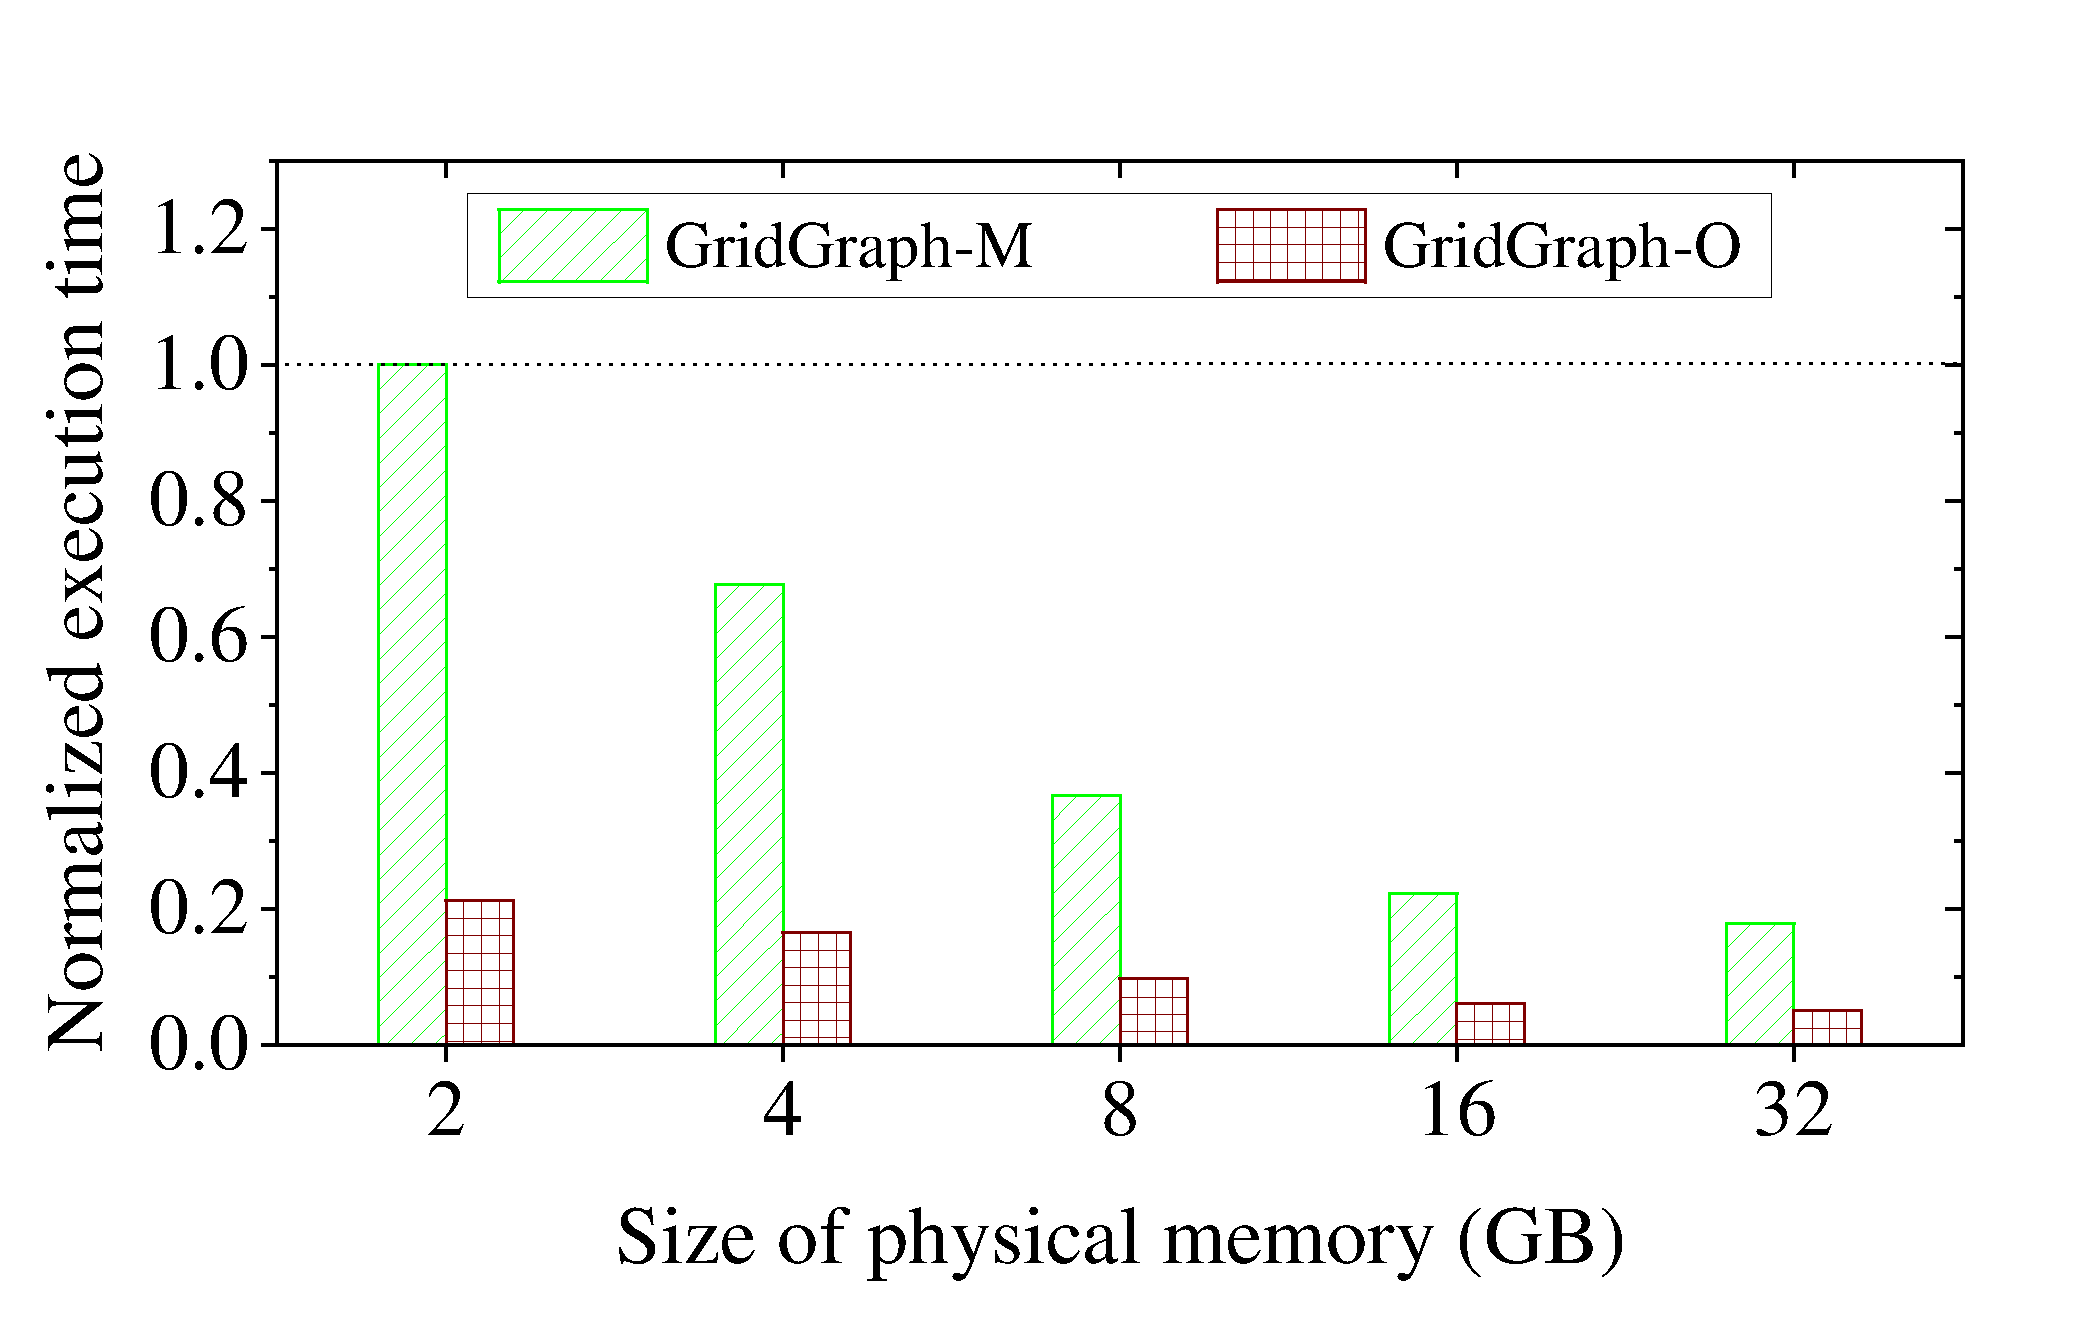
\includegraphics[width=6cm]{Scal_mem.pdf}
%		\vspace{-0.98cm}
%		\caption{Total execution time for adopting the different size of physical memory}
%		\label{Scal_mem}
%	\end{minipage}
%	\hfill
%	\begin{minipage}[t]{0.31\textwidth}
%		\centering
%		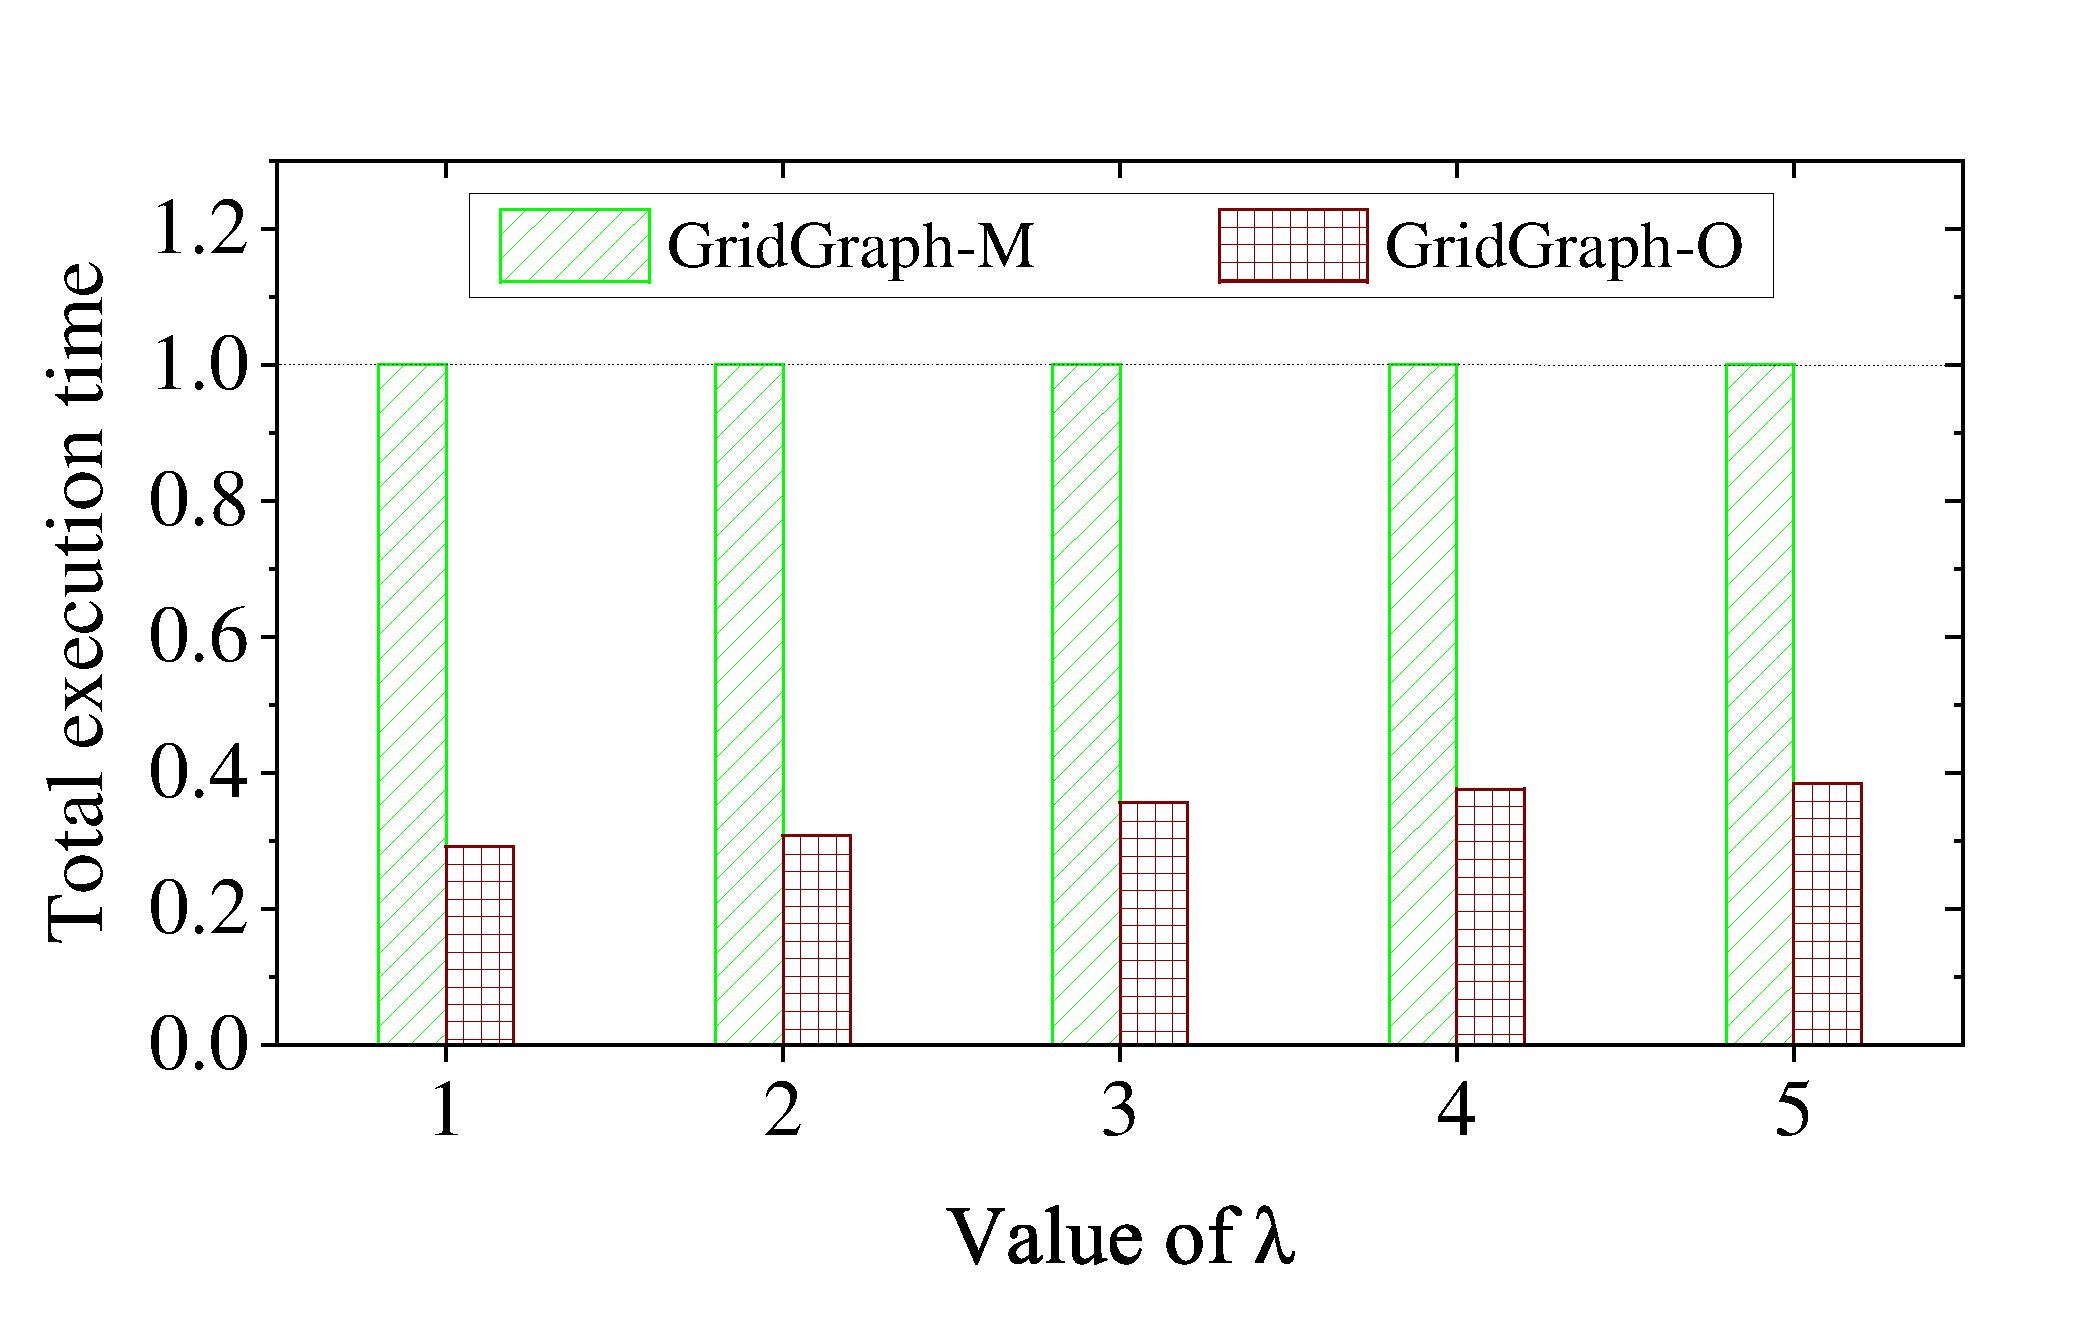
\includegraphics[width=6cm]{Scal_lambda.pdf}
%		\vspace{-0.98cm}
%		\caption{Total execution time when submitting the jobs with different $\lambda$}
%		\label{Scal_lambda}
%	\end{minipage}
%	\vspace{-0.77cm}
%\end{figure*}

\begin{figure*}[t]
	\begin{minipage}[t]{0.31\textwidth}
		\centering
		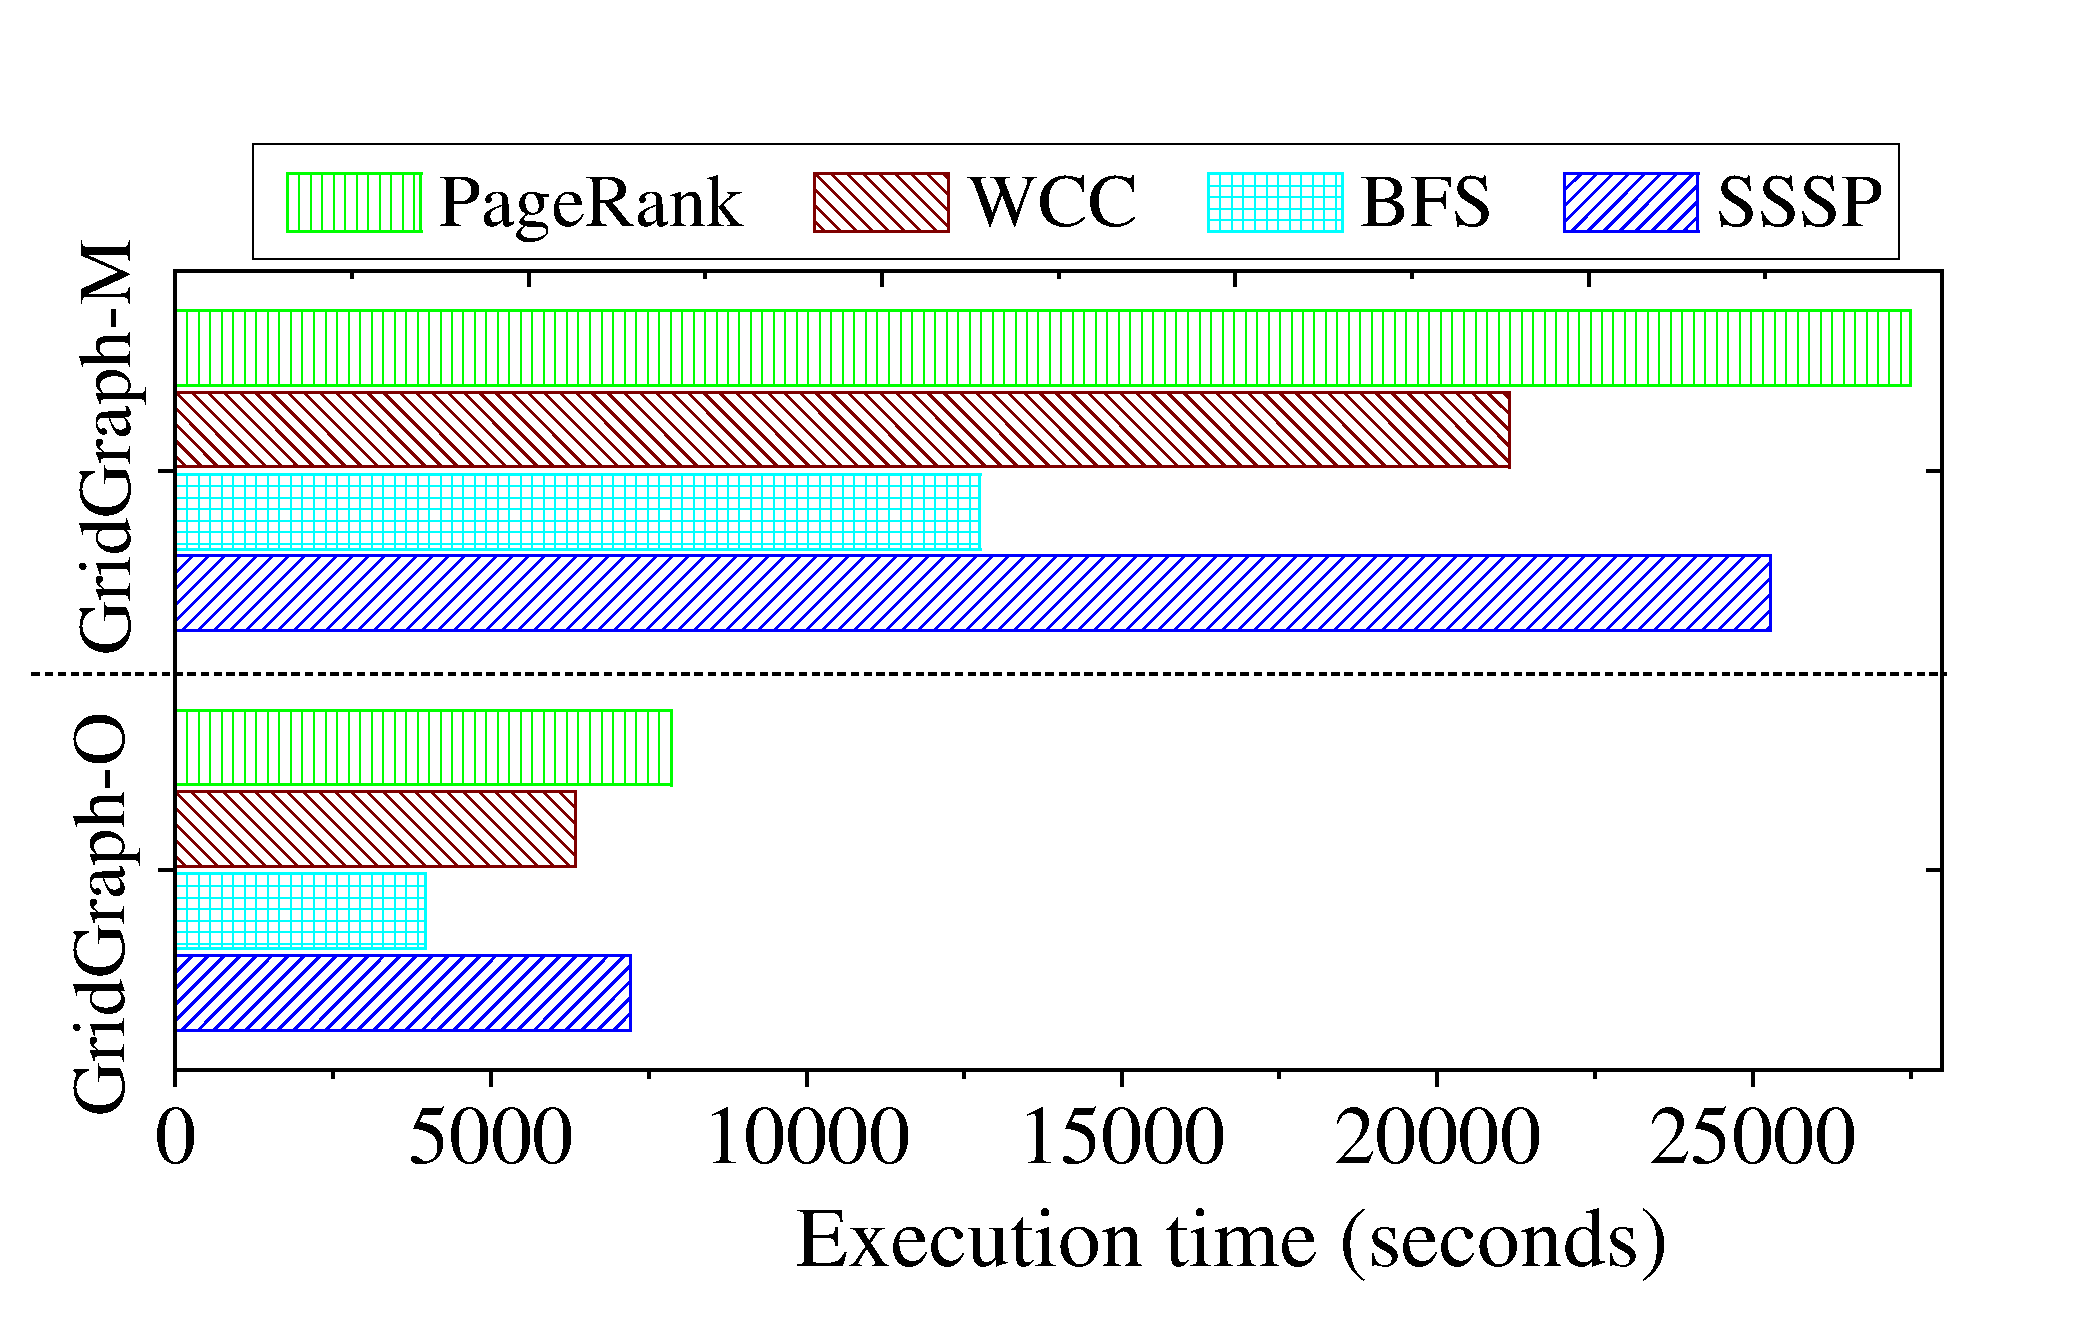
\includegraphics[width=6cm]{deconstruction.pdf}
		\vspace{-0.98cm}
		\caption{Deconstruction of the execution time of the jobs}
		\label{deconstruction}
	\end{minipage}
	\hfill
	\begin{minipage}[t]{0.31\textwidth}
		\centering
		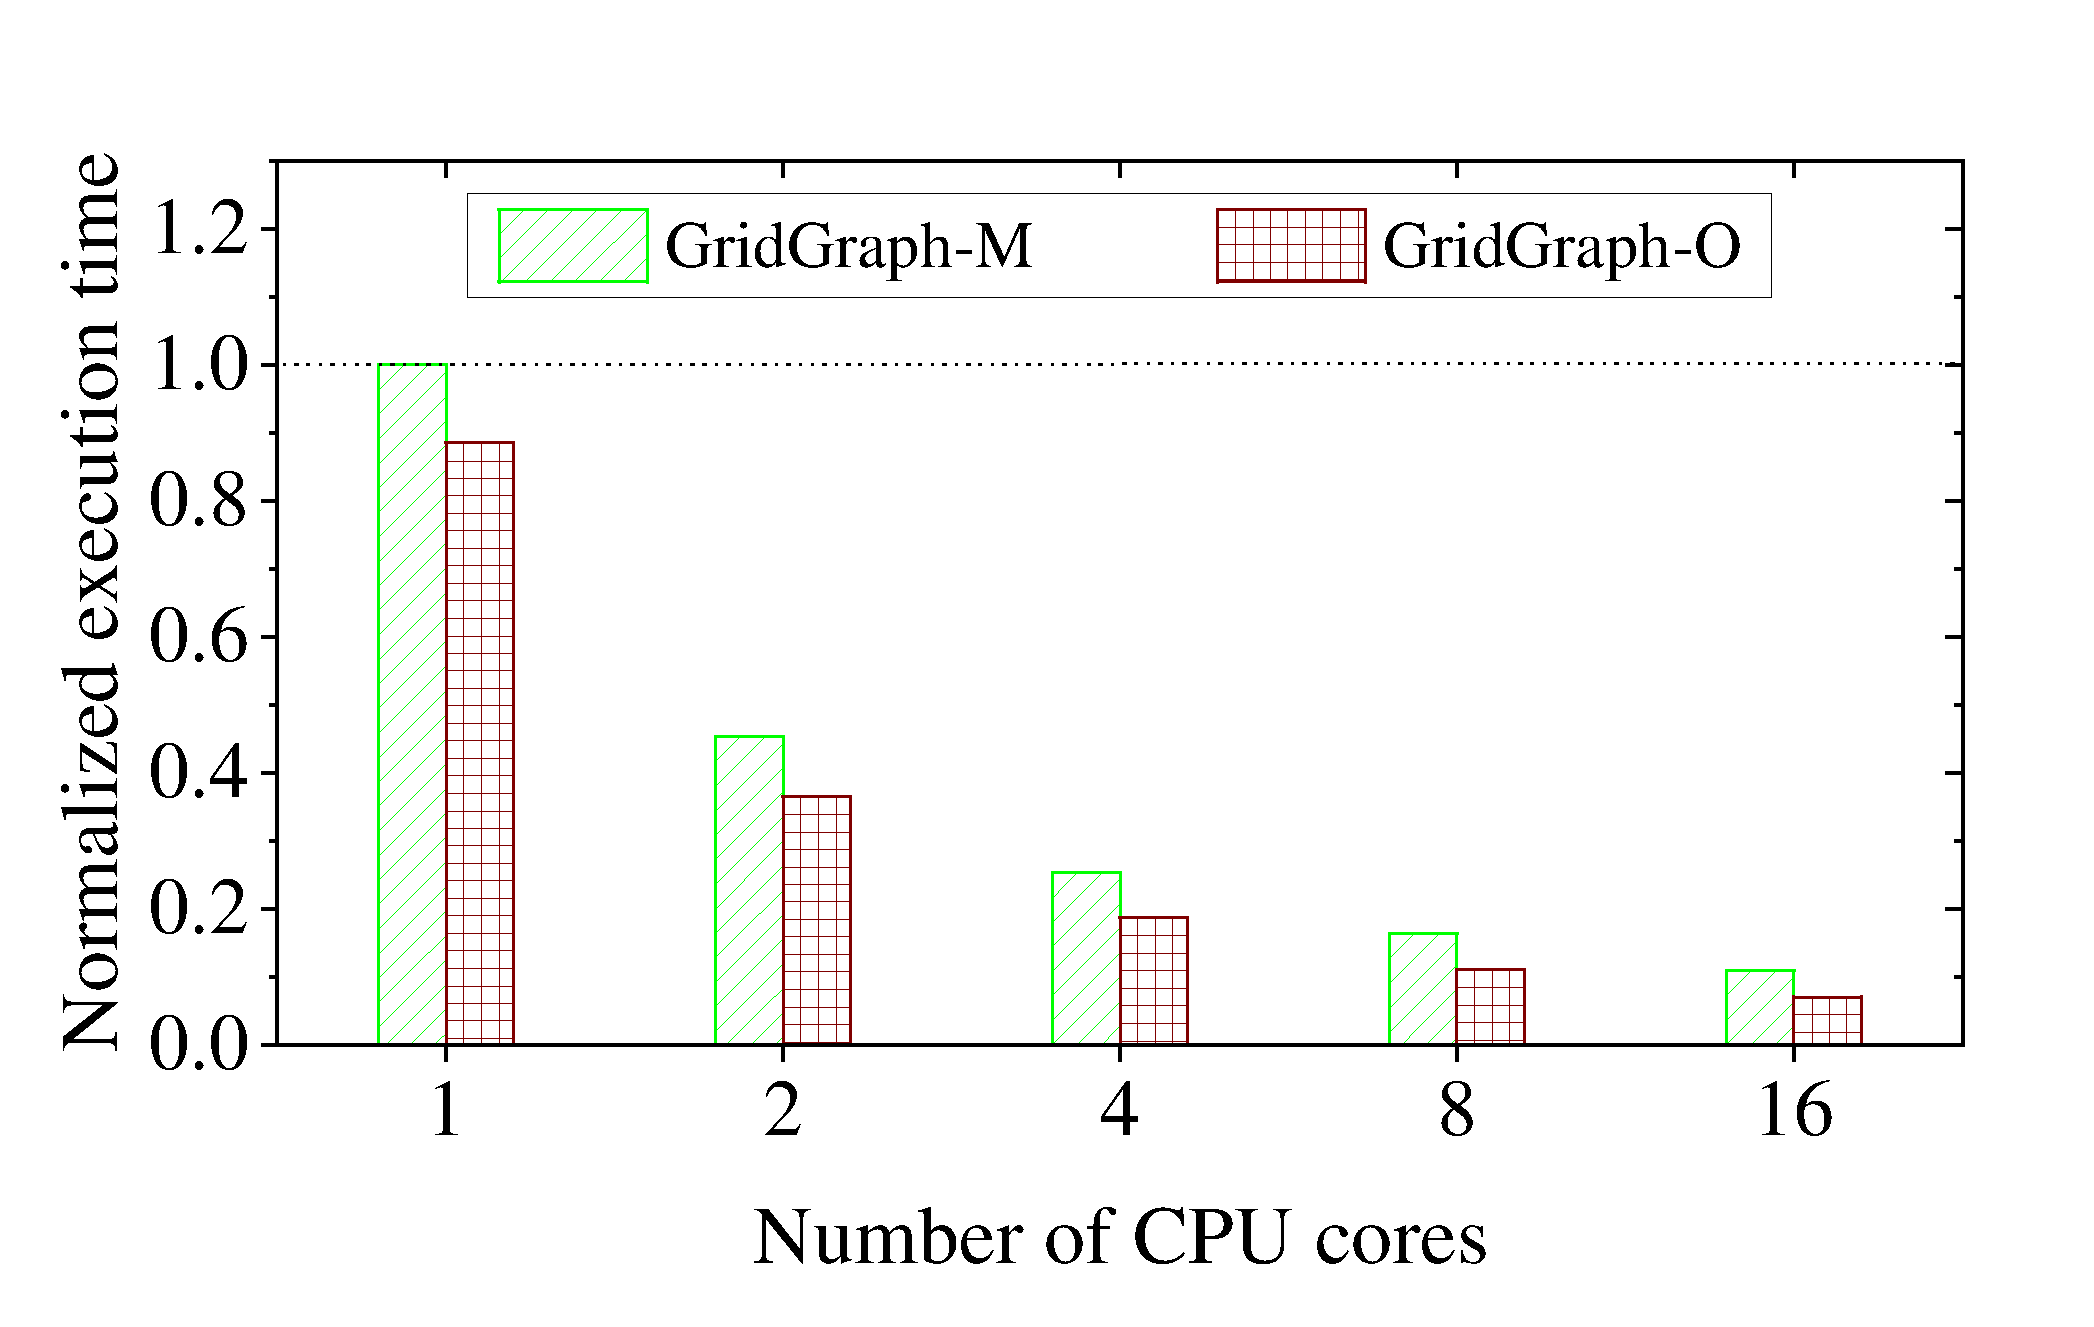
\includegraphics[width=6cm]{Scal_workers.pdf}
		\vspace{-0.98cm}
		\caption{Total execution time for different number of CPU cores}
		\label{Scal_workers}
	\end{minipage}
	\hfill
	\begin{minipage}[t]{0.31\textwidth}
	\centering
	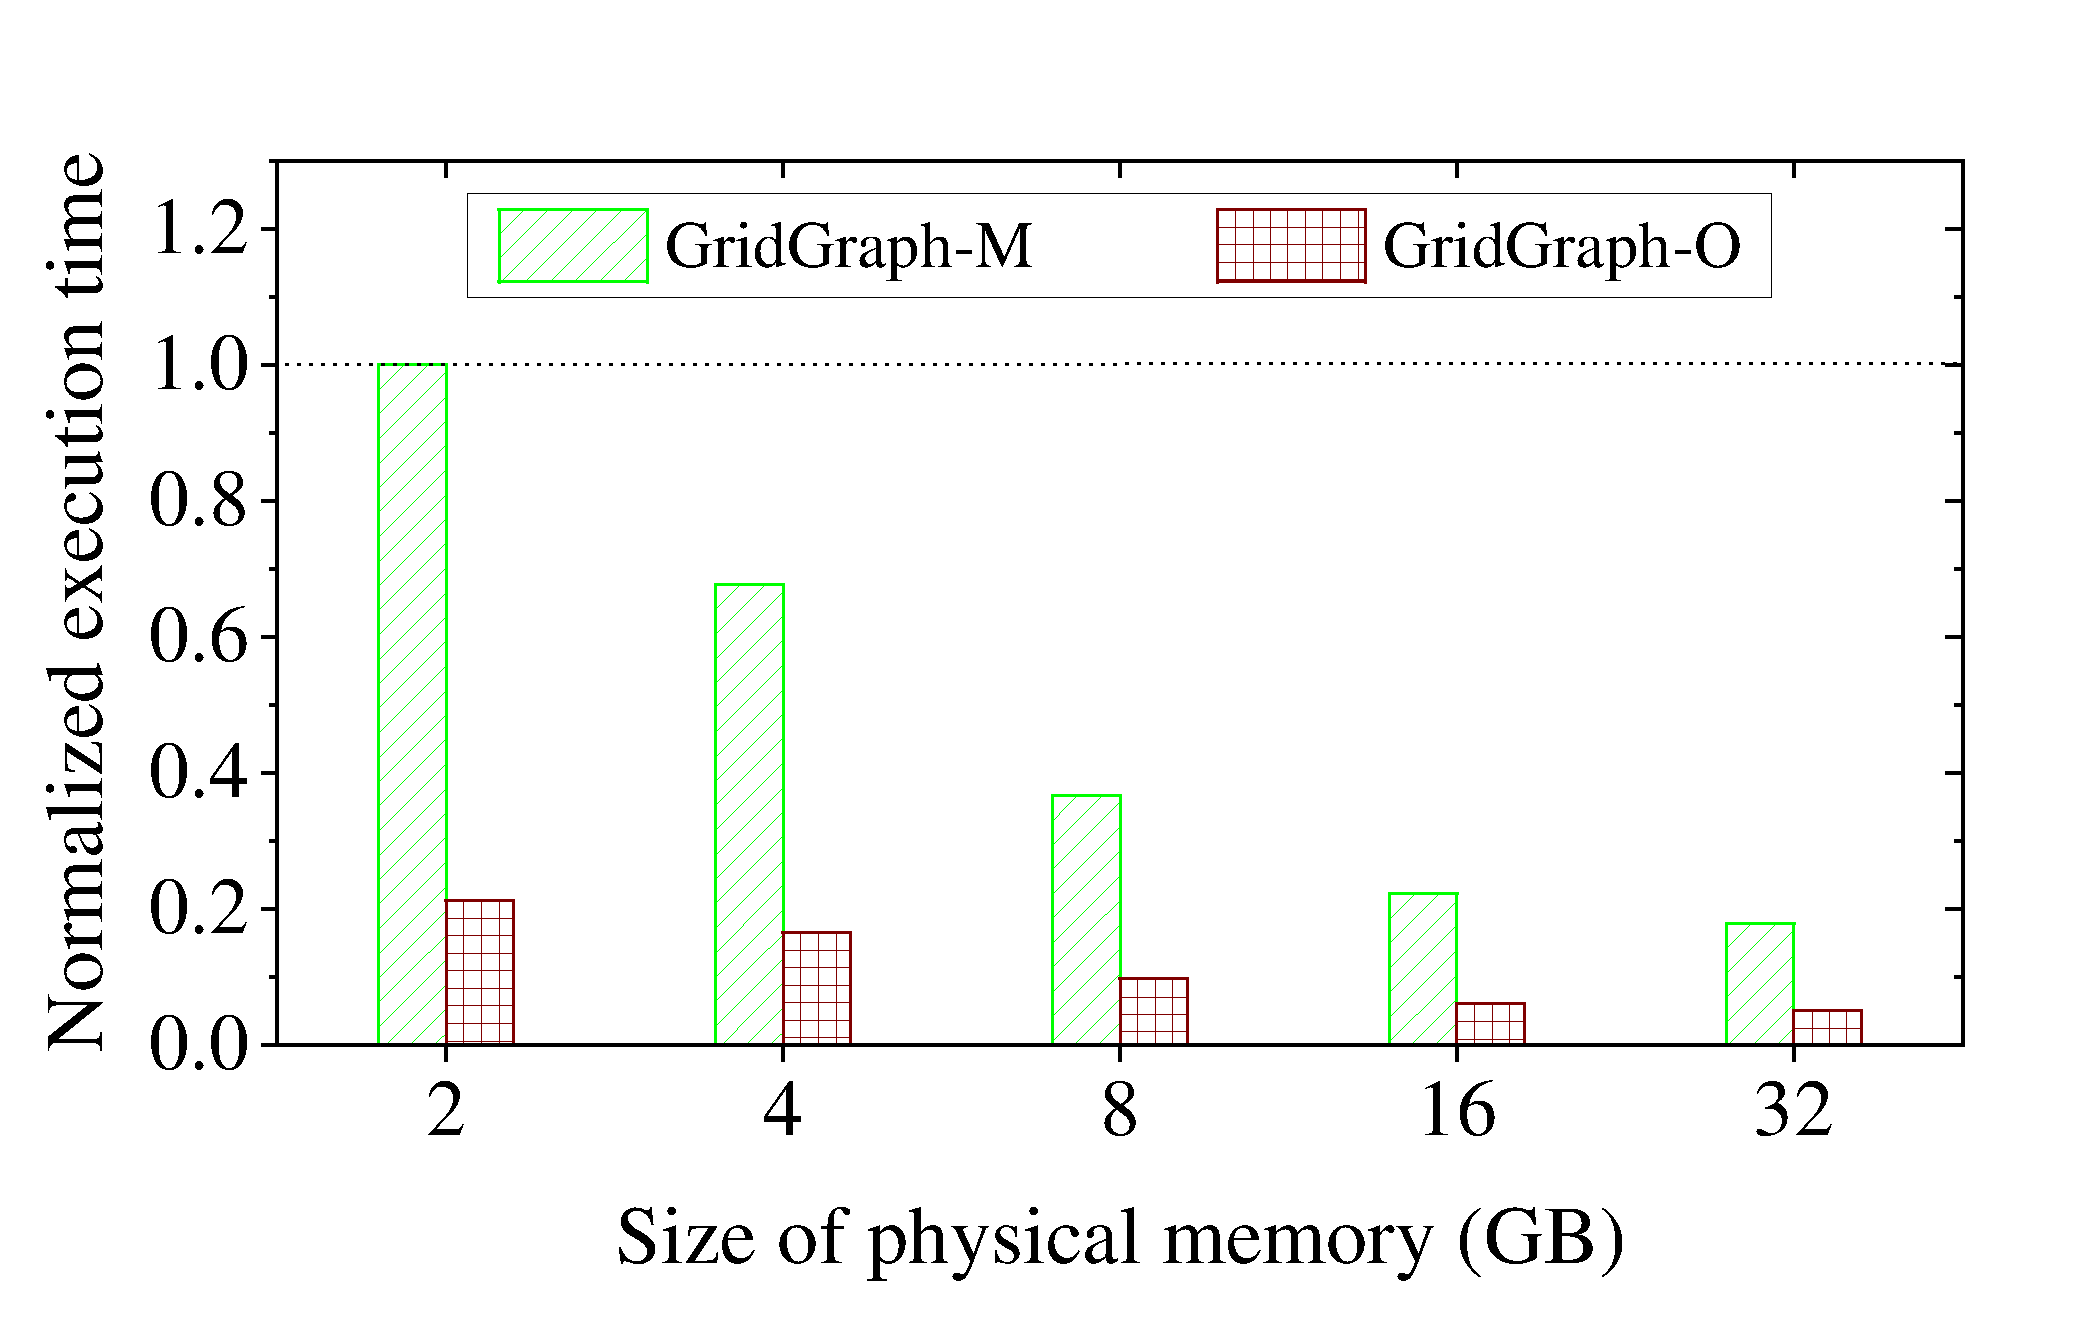
\includegraphics[width=6cm]{Scal_mem.pdf}
	\vspace{-0.98cm}
	\caption{Execution time for adopting different size of physical memory}
	\label{Scal_mem}
	\end{minipage}
	\vspace{-0.77cm}
\end{figure*}

\begin{figure*}[t]
	\begin{minipage}[t]{0.31\textwidth}
	\centering
	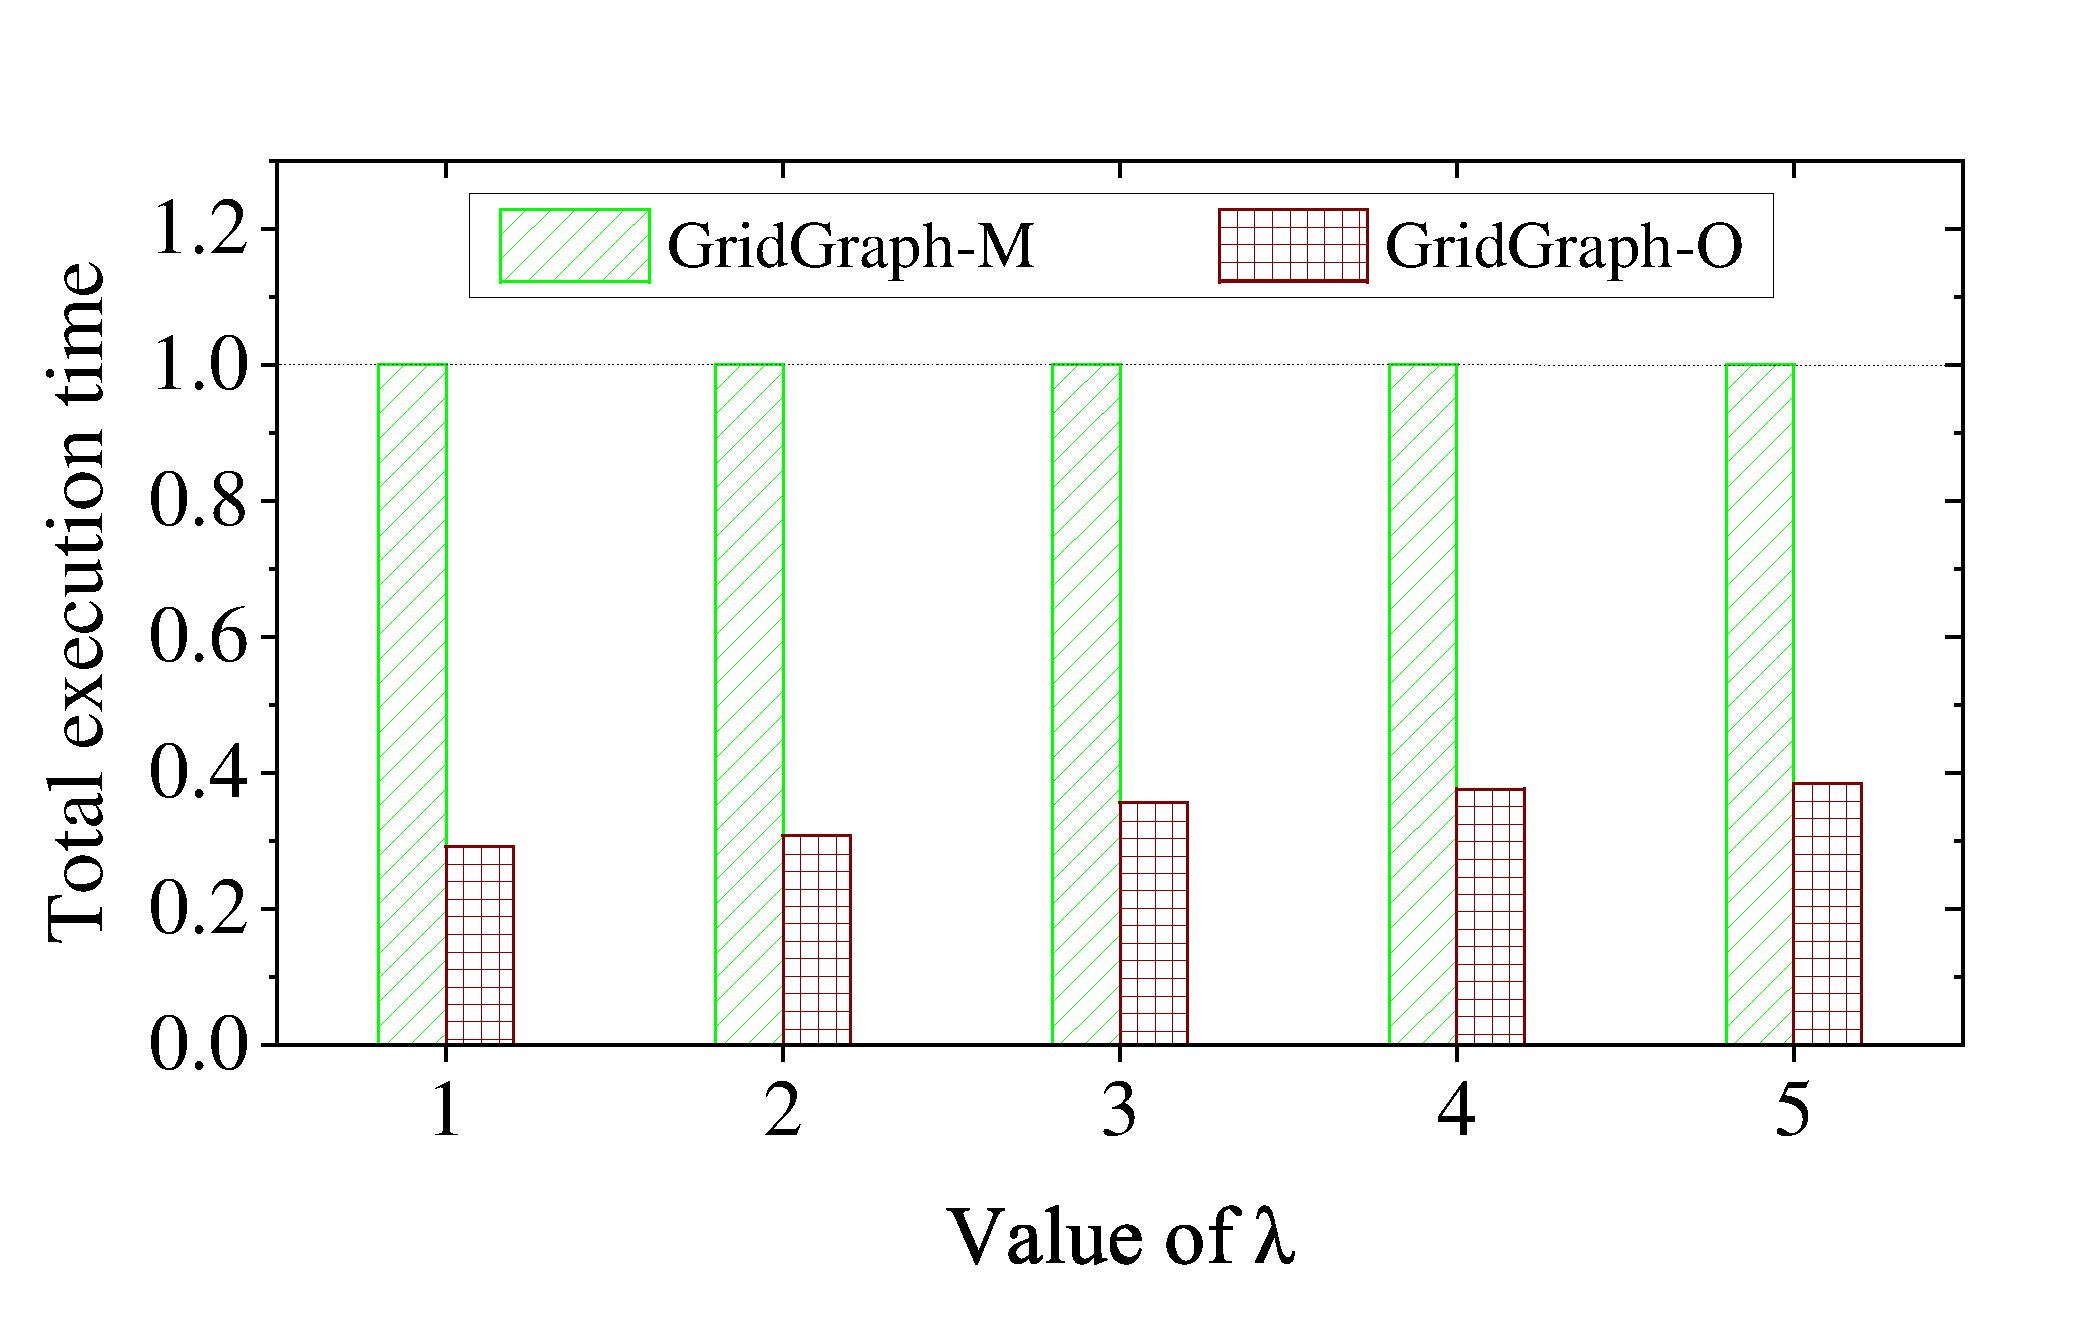
\includegraphics[width=6cm]{Scal_lambda.pdf}
	\vspace{-0.98cm}
	\caption{Total execution time when submitting the jobs with different $\lambda$}
	\label{Scal_lambda}
	\end{minipage}
	\hfill	
	\begin{minipage}[t]{0.31\textwidth}
	\centering
	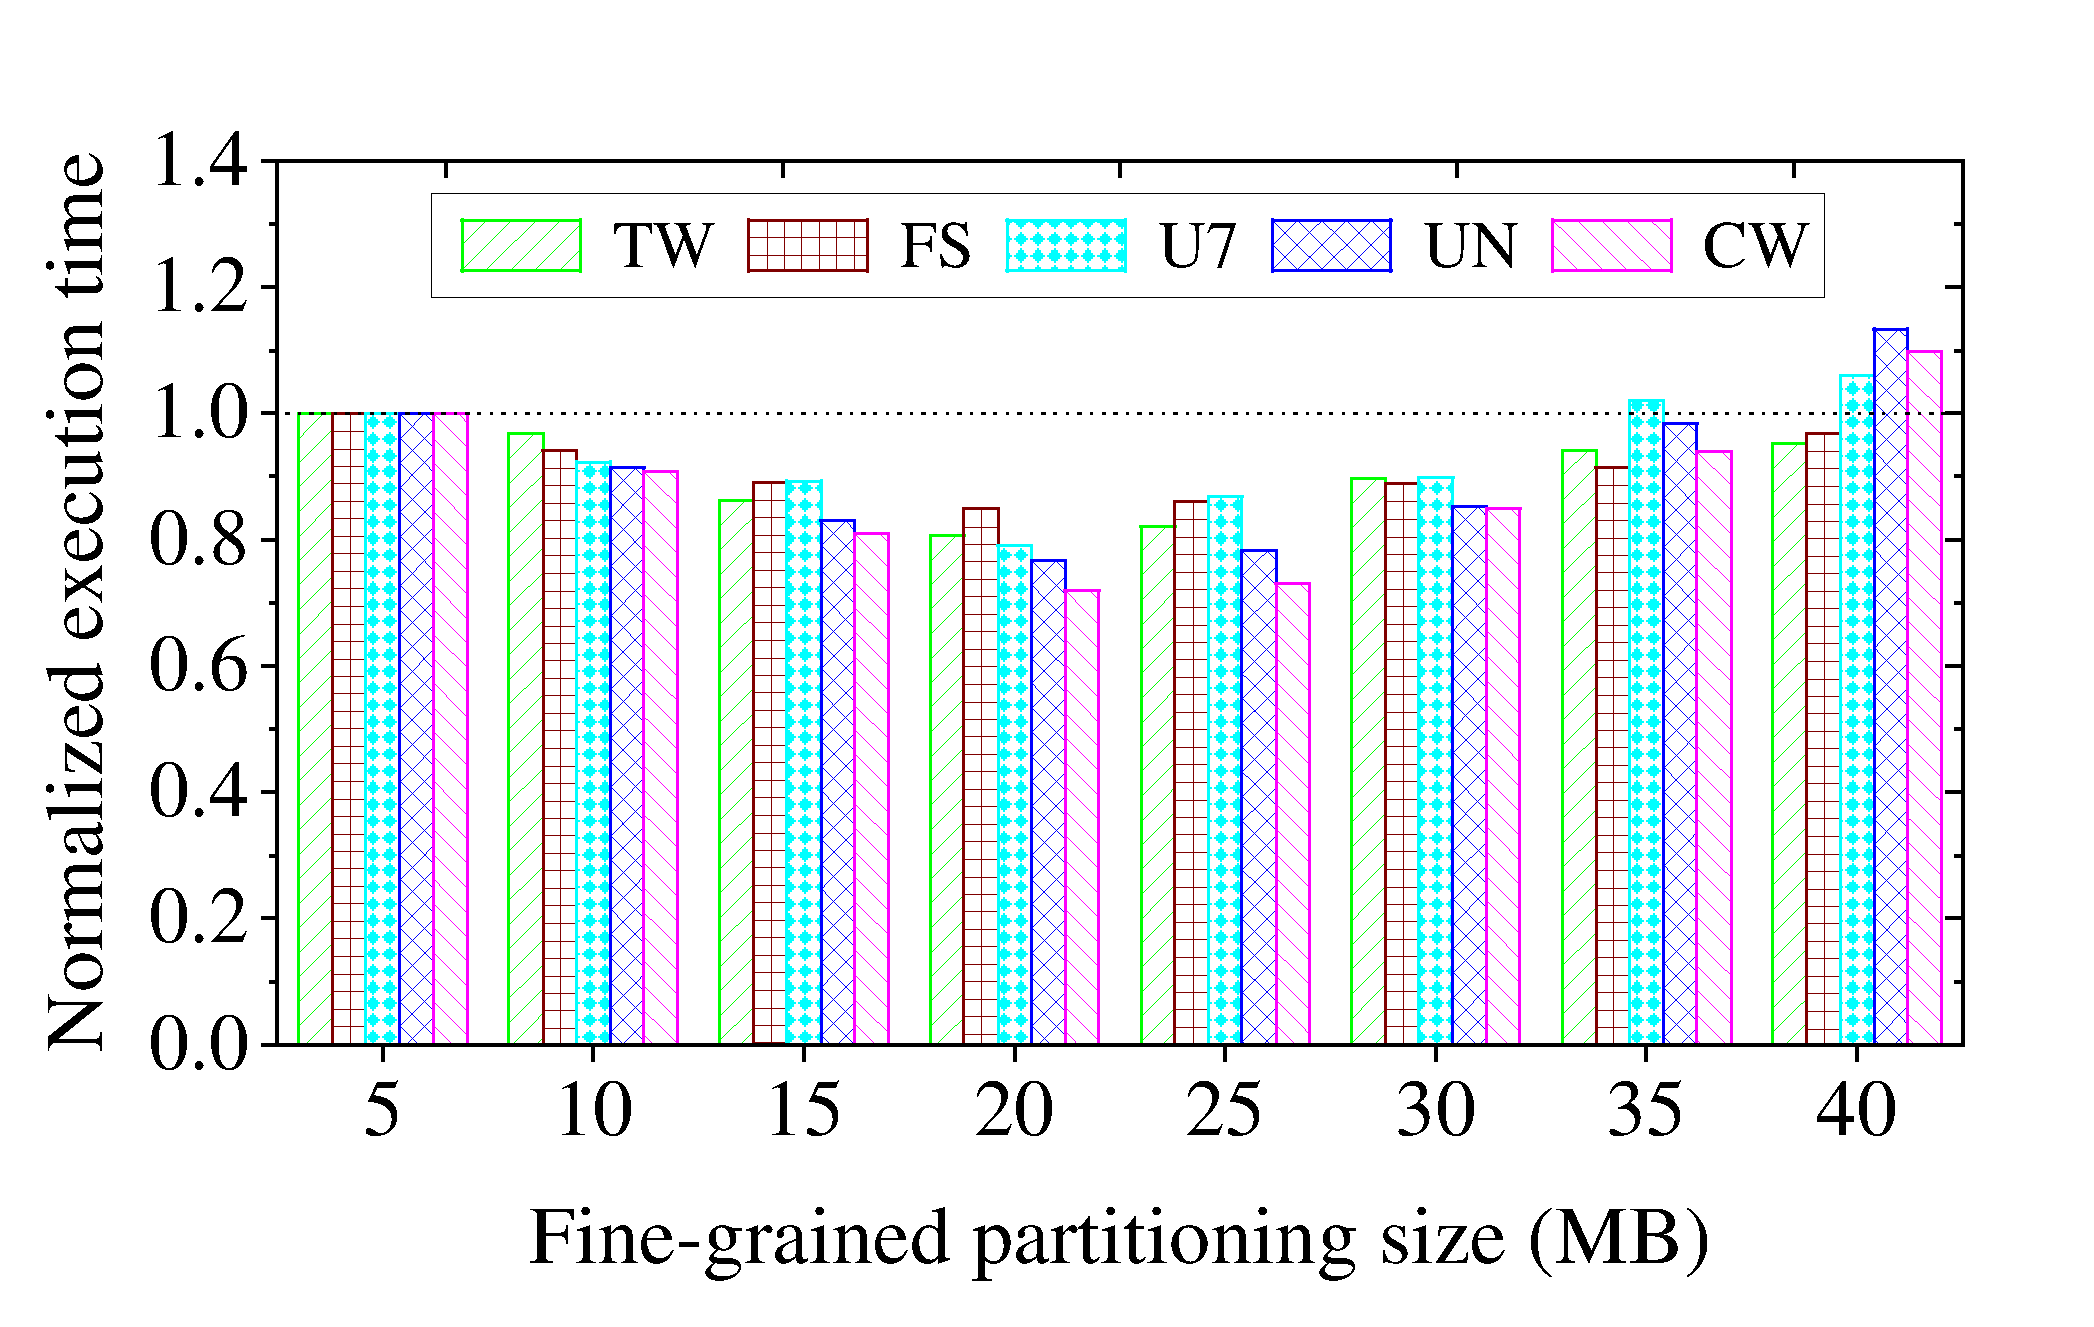
\includegraphics[width=6cm]{Partitioning-size.pdf}
	\vspace{-0.98cm}
	\caption{Total execution time of GridGraph-O with different fine-grained partitioning sizes}
	\label{Partitioning-size}
	\end{minipage}
    \hfill
	\begin{minipage}[t]{0.31\textwidth}
	\centering
	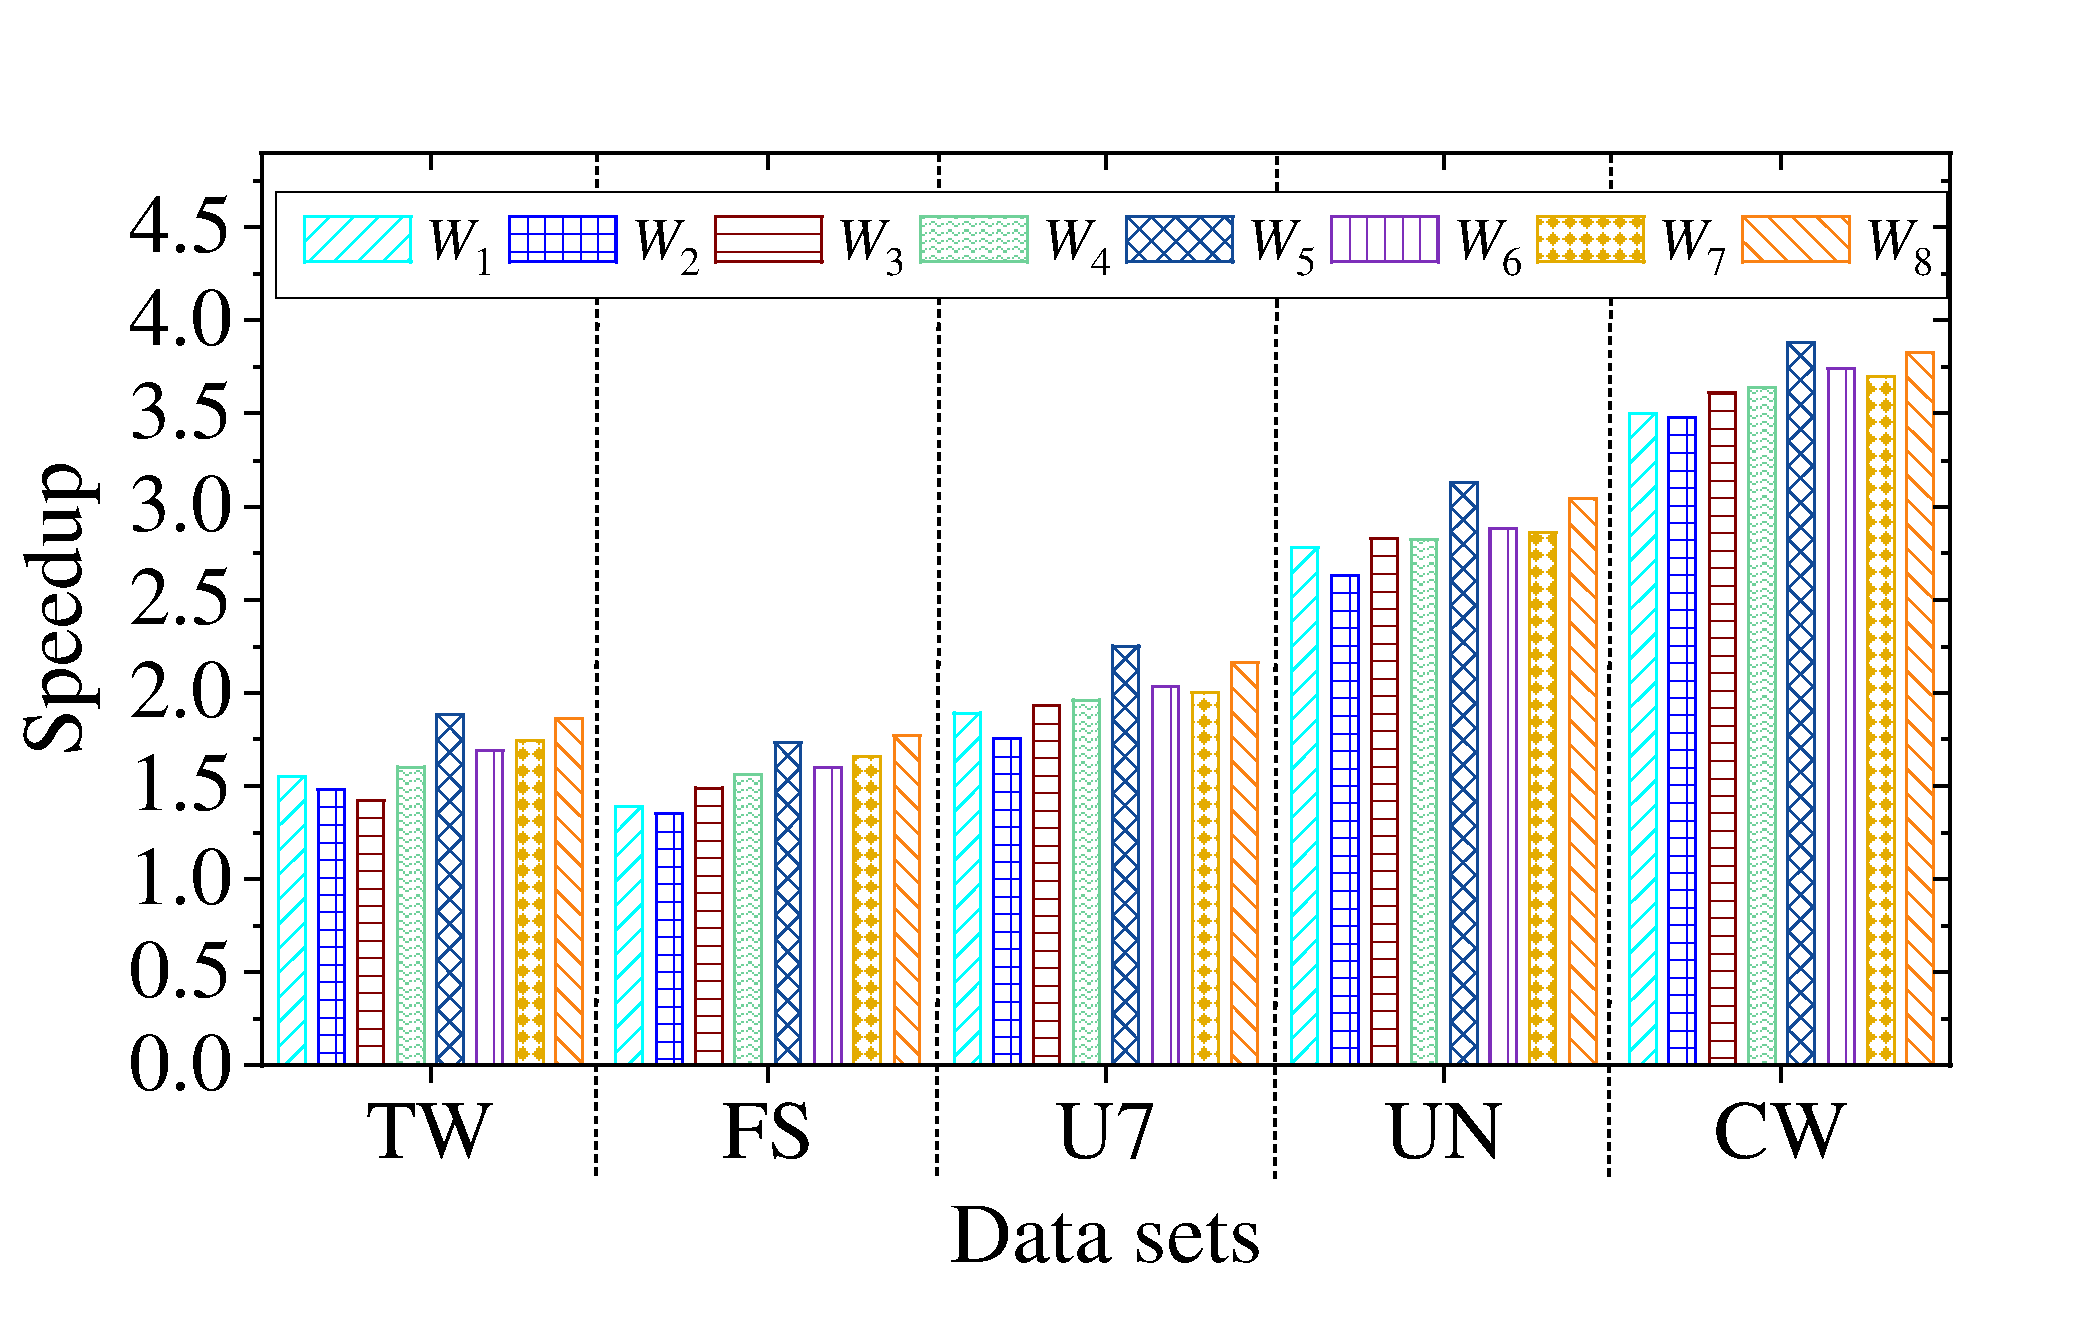
\includegraphics[width=6cm]{Diff-workloads.pdf}
	\vspace{-0.98cm}
	\caption{Performance of GraphSO against GraphM when processing different workloads}
	\label{Diff-workloads}
	\end{minipage}
	\vspace{-0.6cm}
\end{figure*}

\begin{figure}[t]
	\vspace{-10pt}
	\centering
	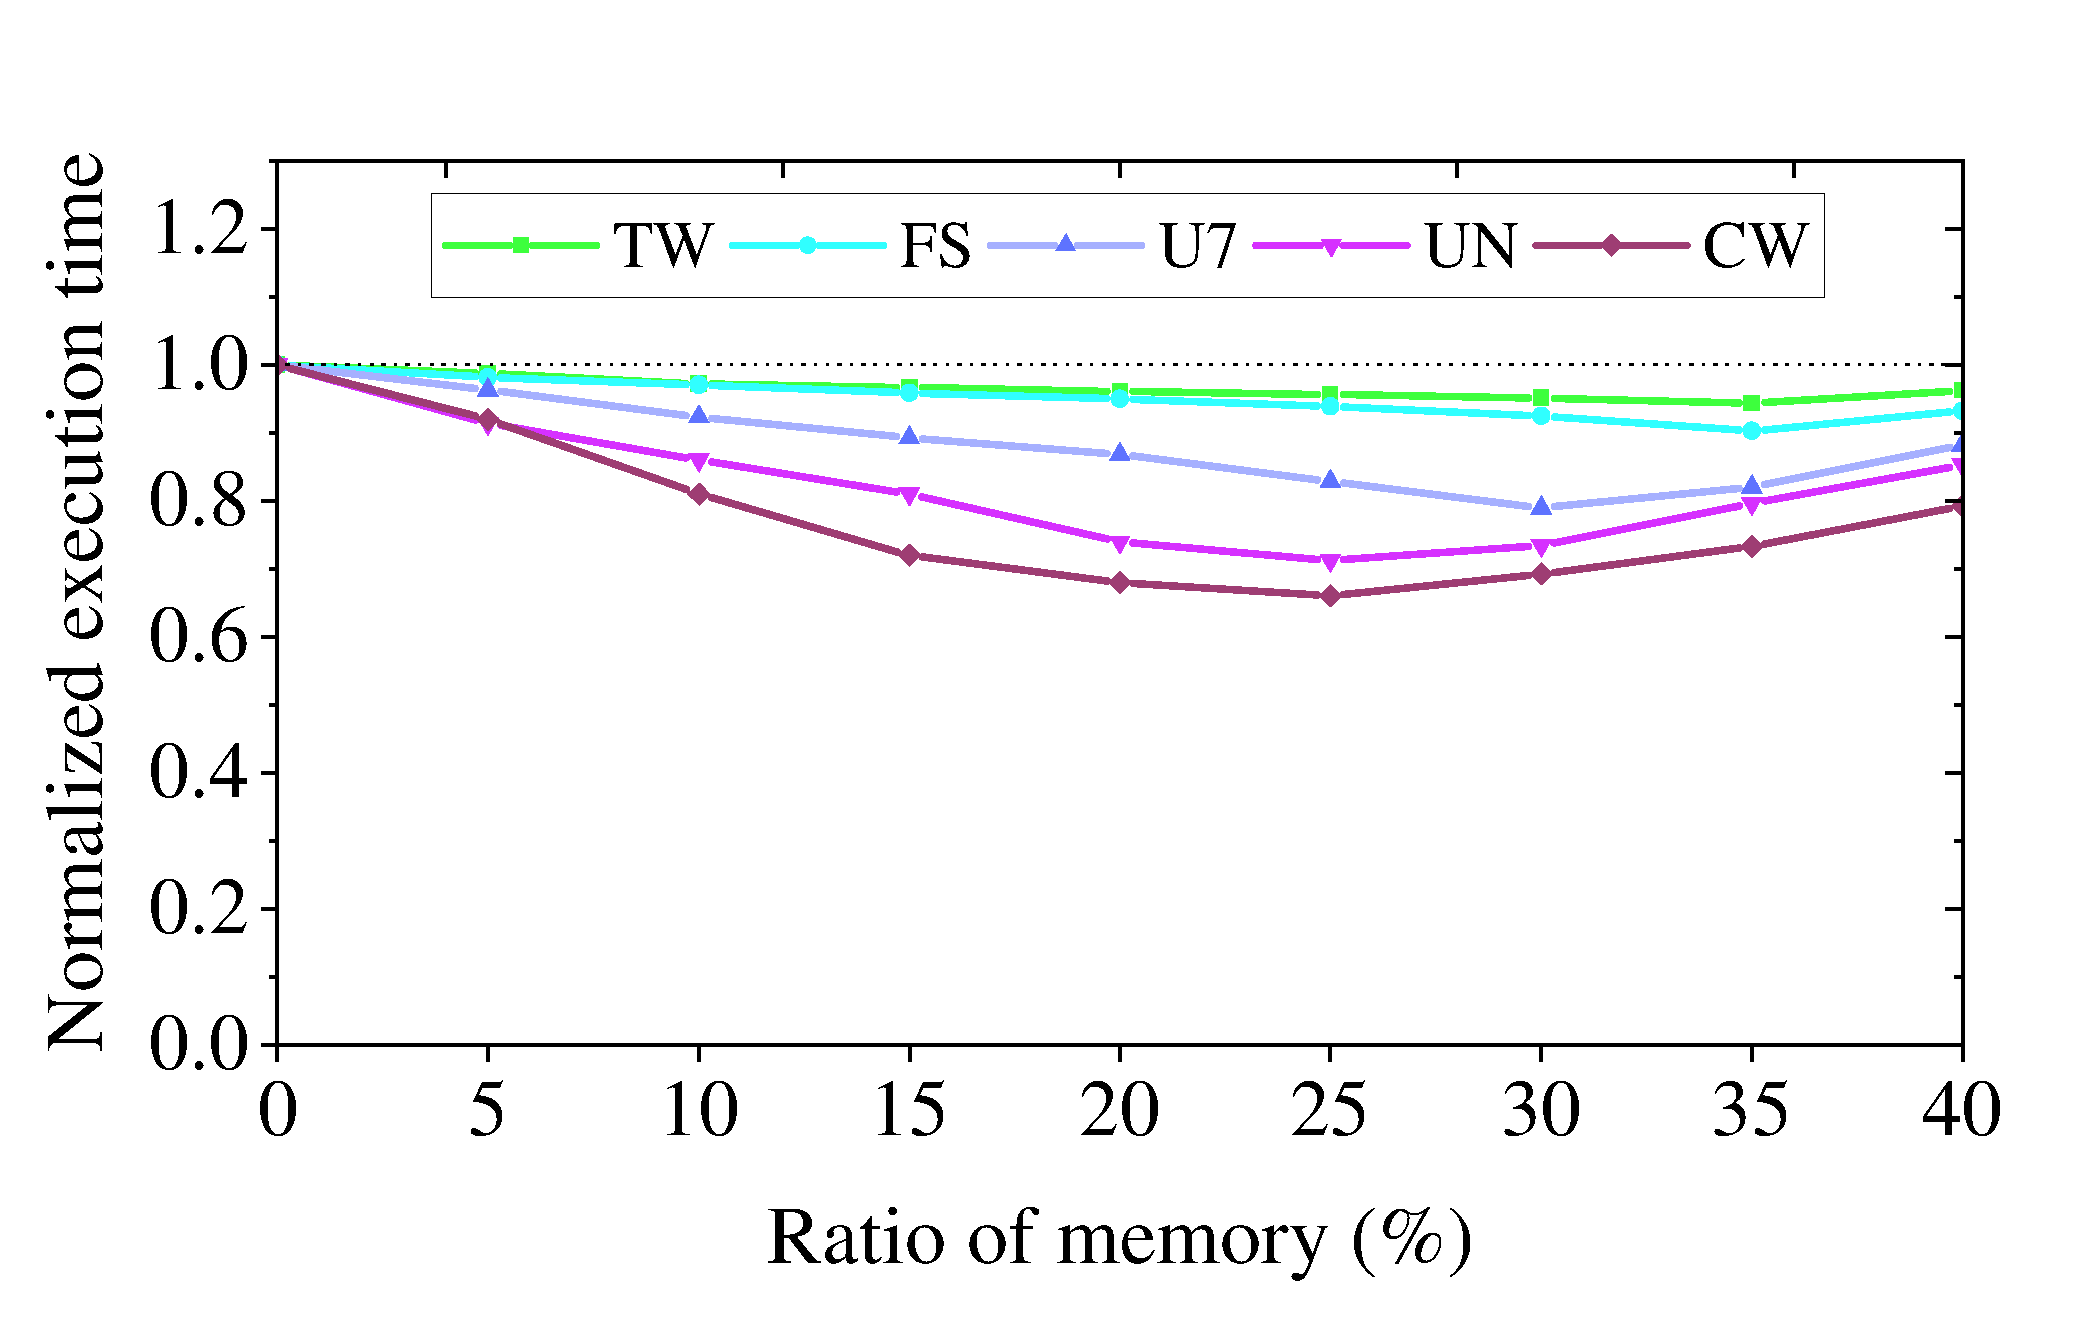
\includegraphics[width=6cm]{memory_size.pdf}
	\vspace{-18pt}
	\caption{Execution time of using various ratios of the main memory to buffer the graph data}
	\label{memory_size}
	\vspace{-24pt}
\end{figure}

%\begin{figure*}[t]
%	\begin{minipage}[t]{0.31\textwidth}
%		\centering
%		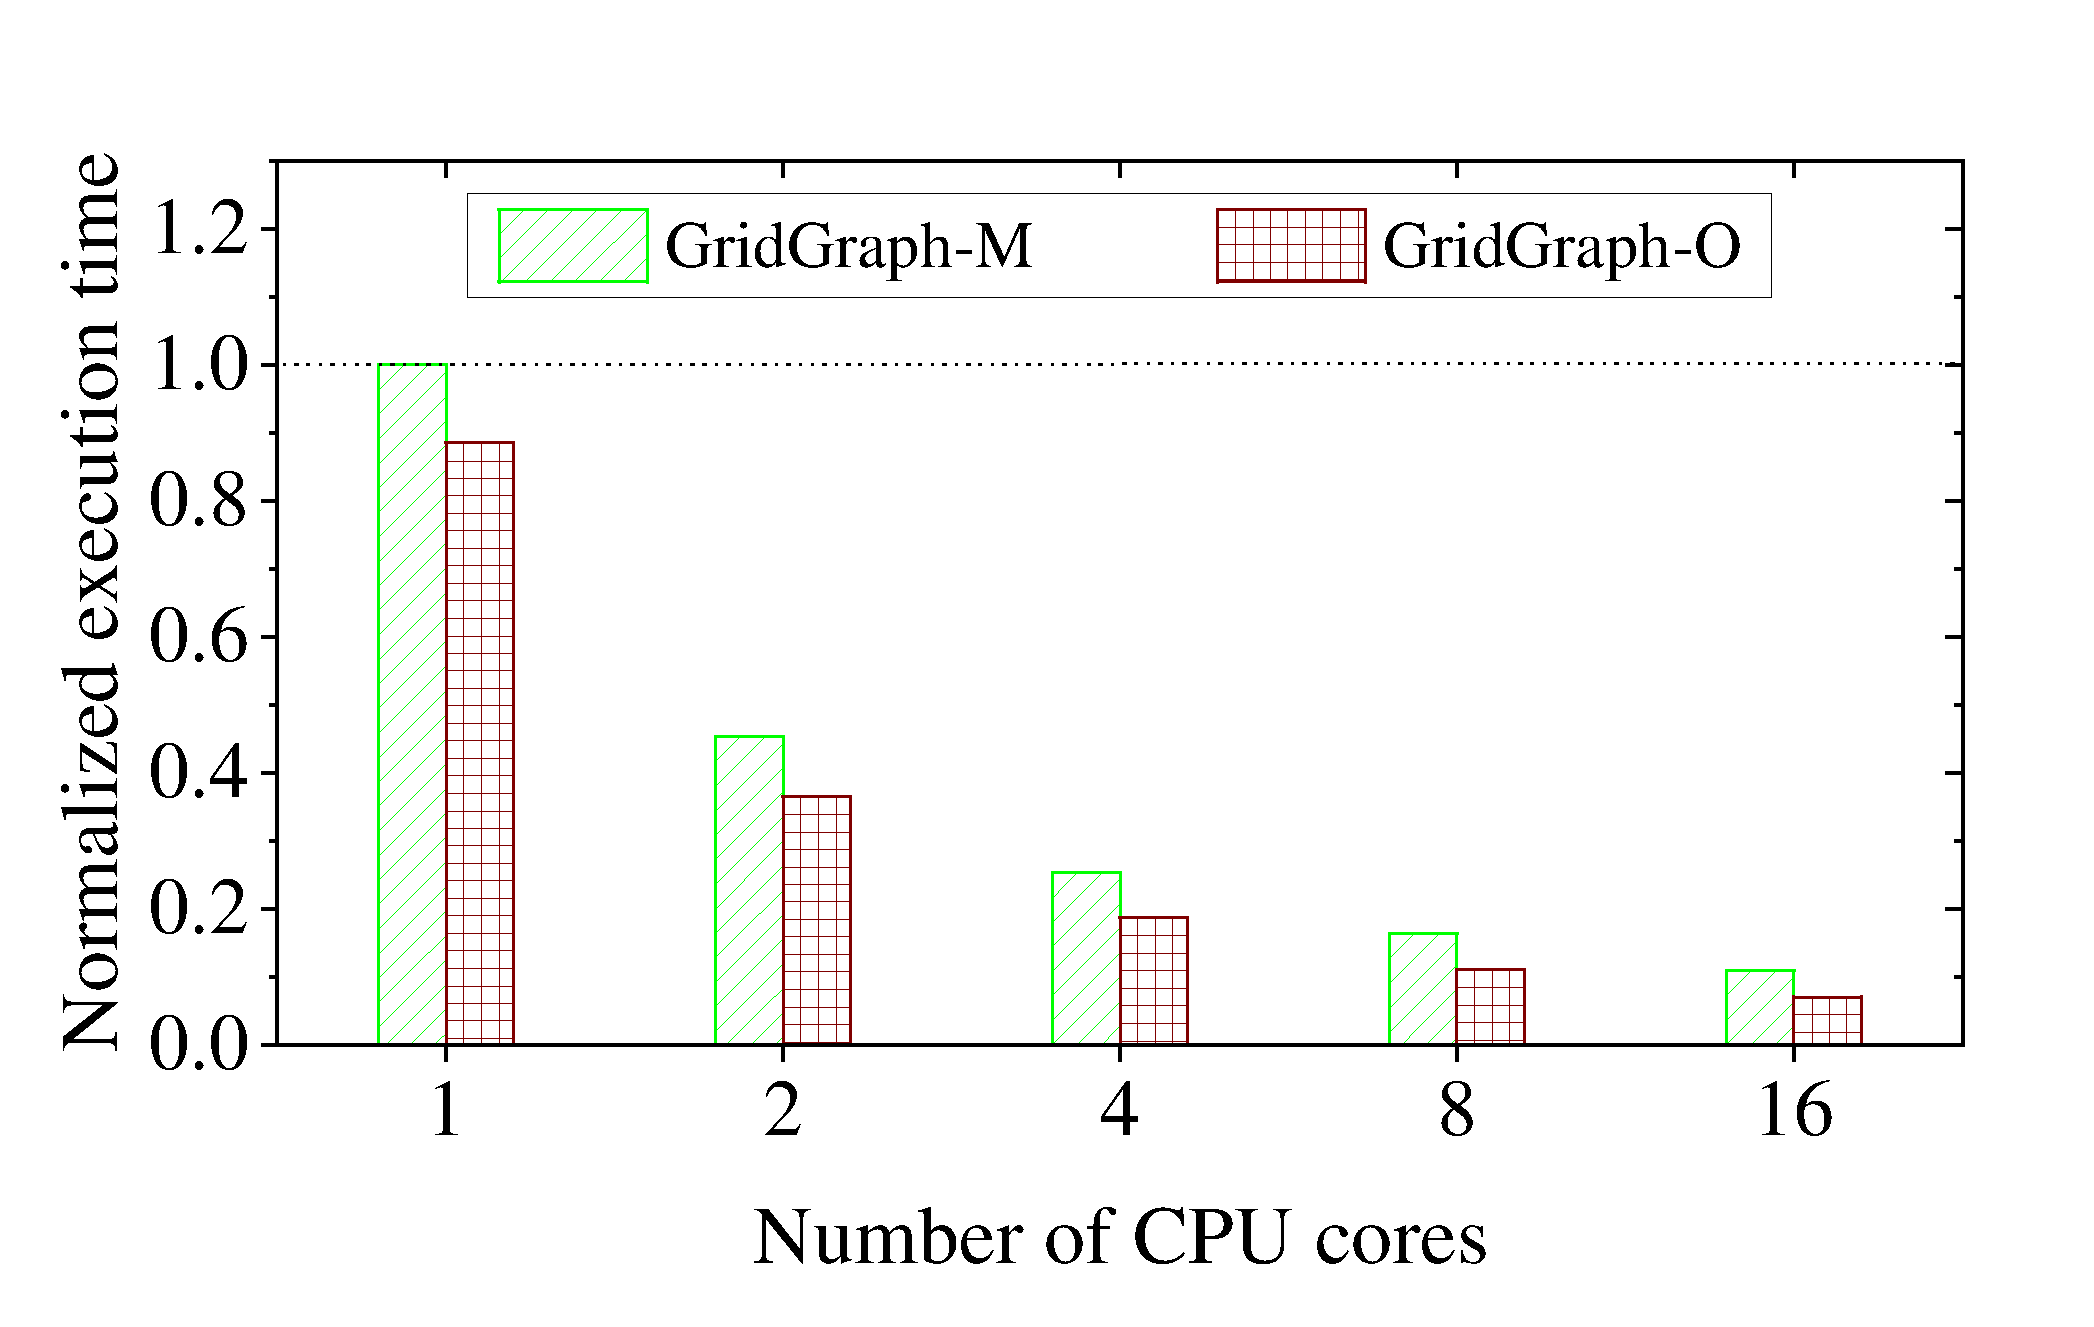
\includegraphics[width=6cm]{Scal_workers.pdf}
%		\vspace{-0.98cm}
%		\caption{Total execution time for different number of CPU cores}
%		\label{Scal_workers}
%	\end{minipage}
%	\hfill
%	\begin{minipage}[t]{0.31\textwidth}
%		\centering
%		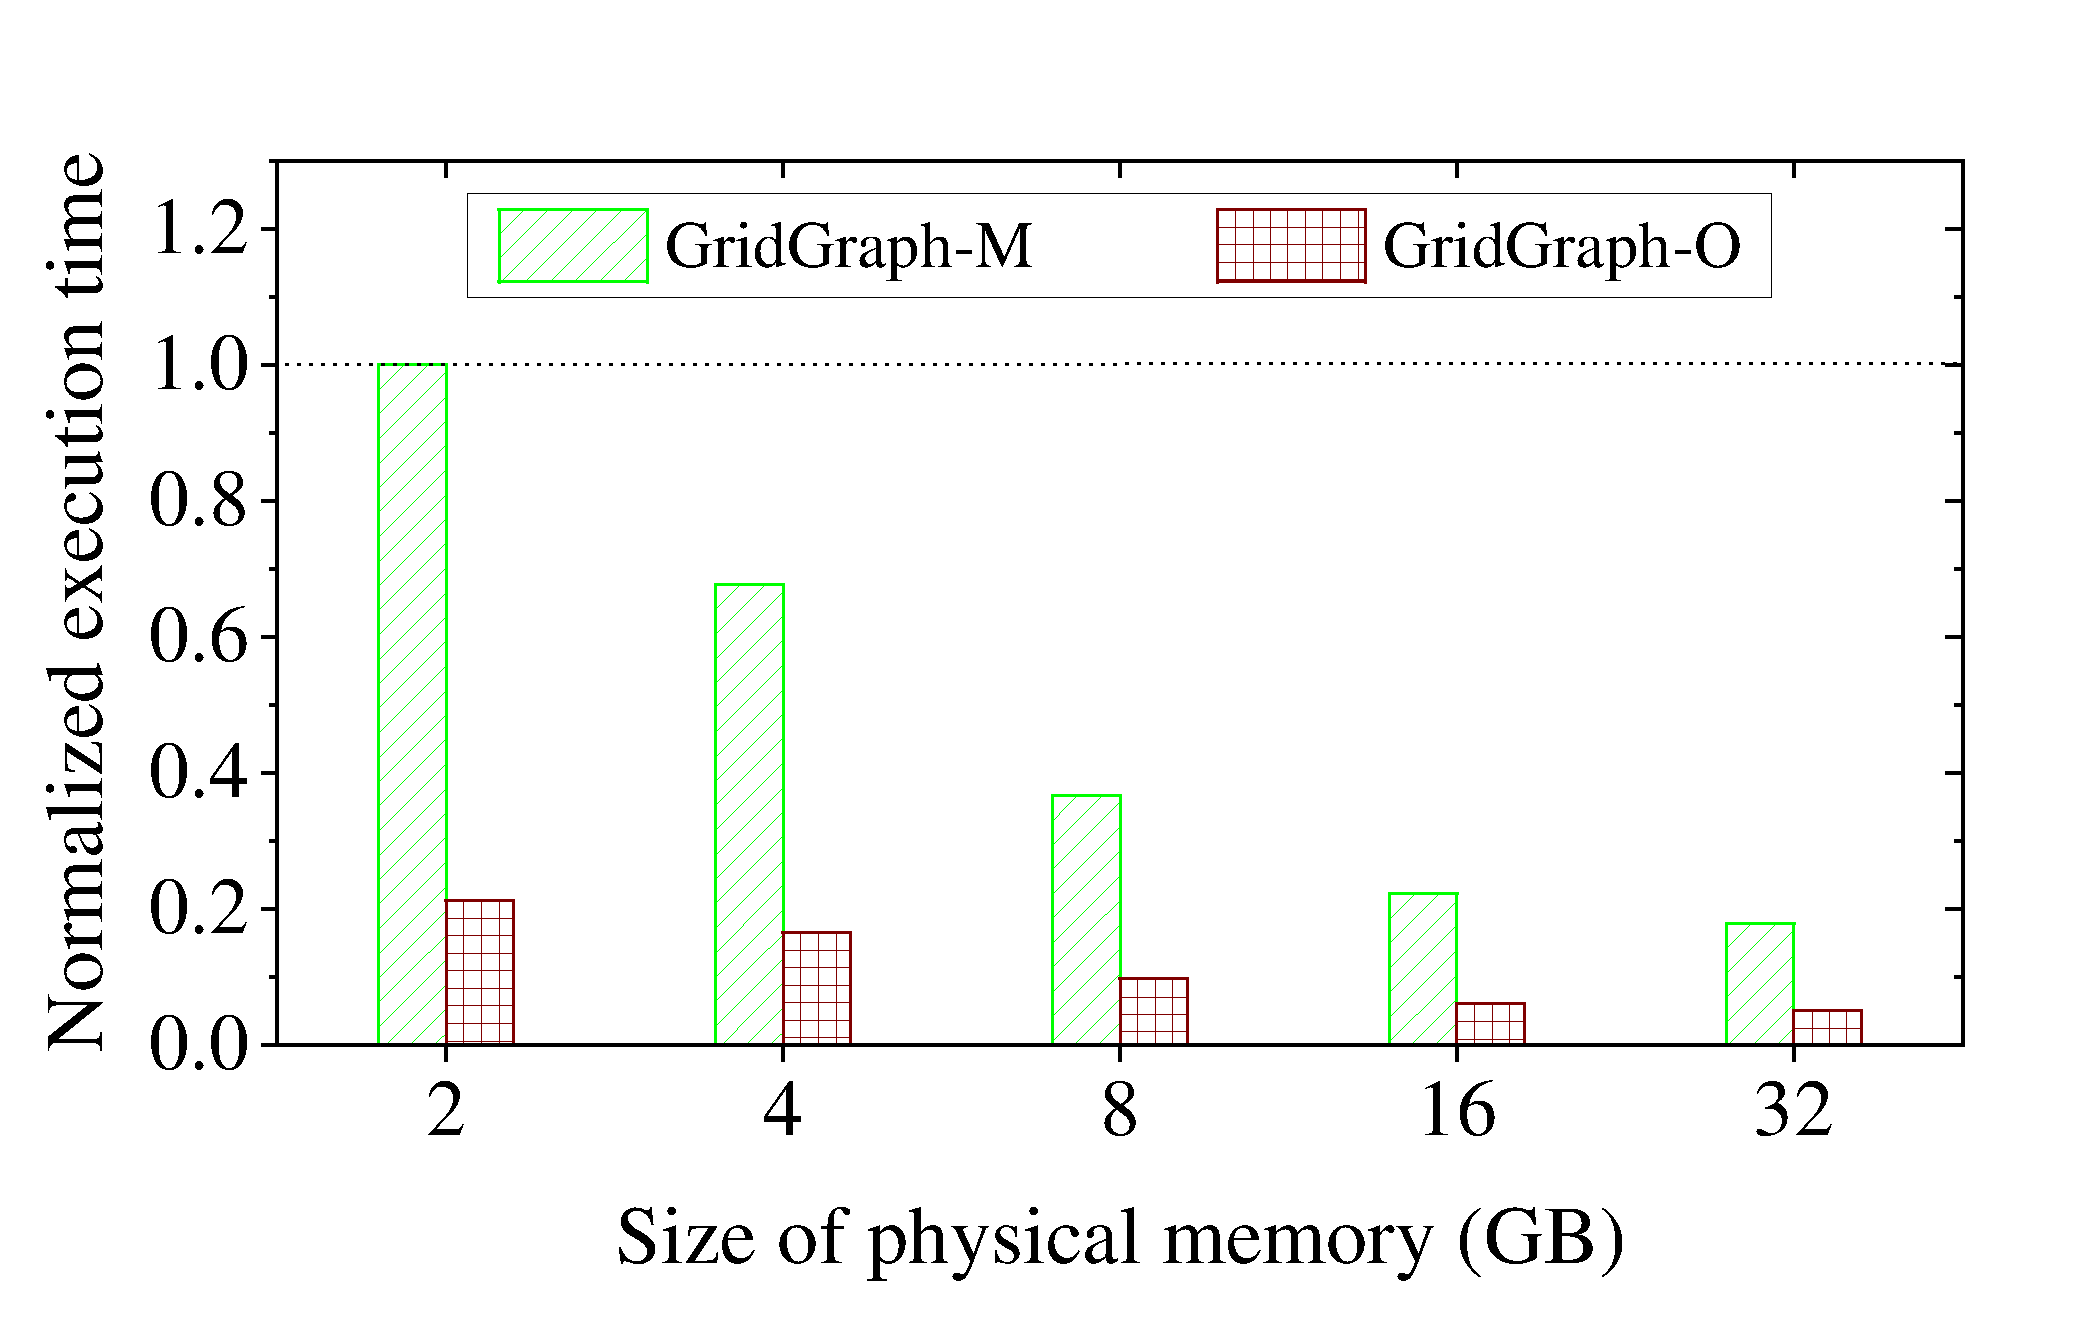
\includegraphics[width=6cm]{Scal_mem.pdf}
%		\vspace{-0.98cm}
%		\caption{Total execution time for adopting the different size of physical memory}
%		\label{Scal_mem}
%	\end{minipage}
%	\hfill
%	\begin{minipage}[t]{0.31\textwidth}
%		\centering
%		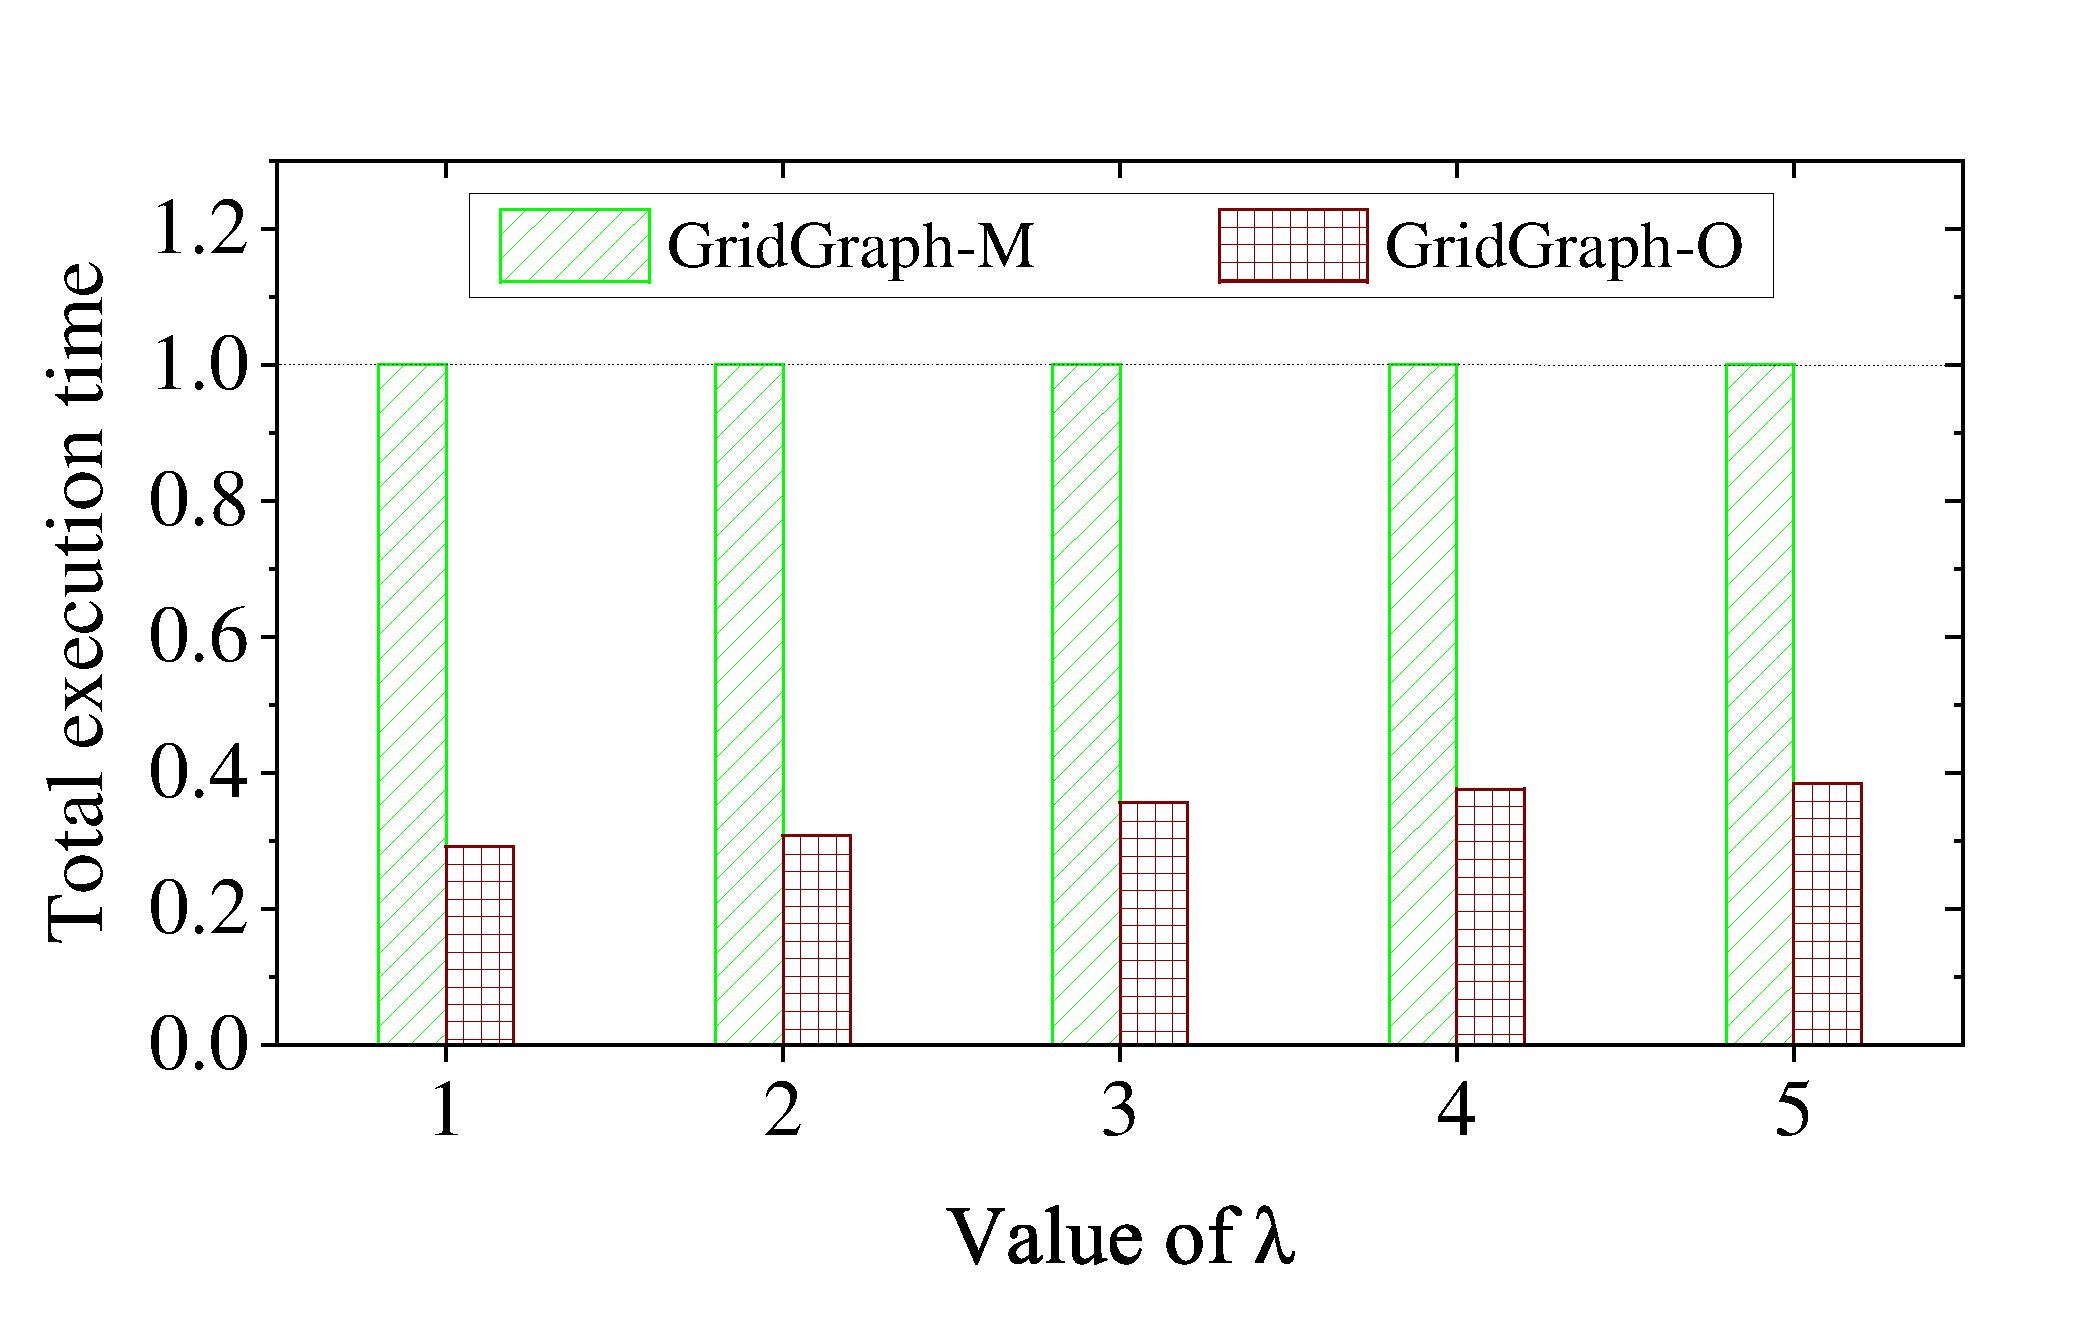
\includegraphics[width=6cm]{Scal_lambda.pdf}
%		\vspace{-0.98cm}
%		\caption{Total execution time when submitting the jobs with different $\lambda$}
%		\label{Scal_lambda}
%	\end{minipage}
%	\vspace{-0.77cm}
%\end{figure*}


\vspace{-8pt}
\subsection{Overall Performance}
\vspace{-2pt}
To compare GridGraph-M and GridGraph-O, we concurrently submit SSSP, PageRank, BFS, and WCC as four concurrent jobs to different schemes. The normalized results are depicted in Fig.~\ref{exe_time}.
For TW, FS, U7, UN, and CW, the execution time of the baseline system (i.e., GridGraph-M) is 295, 378, 1,585, 2,071, and 27,493 seconds, respectively.
It shows that GridGraph-O requires shorter execution time to run the four jobs than GridGraph-M. This indicates that higher throughput is achieved by GraphSO. For example, comparing with GridGraph-M, GridGraph-O improves the throughput by 3.5 times over CW dataset. The throughput improvement basically results from the lower I/O overhead brought by GraphSO. Note that the synchronization overhead (i.e., synchronizing multiple jobs to process the same chunks) occupies 6.3\%-12.1\%, and the chunk management cost (e.g., identifying active chunks and constructing logical partitions) occupies 3.8\%-6.7\% of the total execution time of the jobs on GridGraph-O for our test instances.

We breakdown the execution time for running the four jobs on various schemes in Fig.~\ref{breakdown}. It shows that, compared with GridGraph-M, the graph processing time of jobs on GridGraph-O occupies a larger ratio of the total execution time. This means that GridGraph-O requires less data access time. For example, over CW dataset, the data accessing time of GridGraph-O is reduced by 4.6 times compared with GridGraph-M. The lower data access time brought by GraphSO is caused by the following reasons. First, it loads  less graph data into the memory, because the loading of much unnecessary graph data (i.e., inactive fine-grained chunks in active coarse-grained partitions) is bypassed and each loaded logical partition (i.e., a set of active chunks) is fully utilized by concurrent jobs.
%important chunks are flexibly cached in the memory to be reused by concurrent jobs during the execution.
Second, the processing of inactive chunks is skipped in each iteration,  resulting in less graph data steamed into the LLC.

In order to prove it, we trace the total I/O traffic for executing the four jobs on various schemes. Fig.~\ref{IO} shows the normalized results of GridGraph-O against GridGraph-M. As described, compared to GridGraph-M, less I/O overhead is produced by GridGraph-O, especially as the graph size is larger than the physical memory size. For instance, the I/O cost of GridGraph-O is only 21.6\% of GridGraph-M over CW dataset, because GraphSO eliminates much unnecessary I/O traffic via repartitioning static partitions and maximizing the utilization of loaded graph data. On the contrary, although GraphM can reduce the redundant I/O overhead by sharing the same graph data for concurrent jobs, much unnecessary graph data are also loaded for concurrent jobs, leading to severe I/O inefficiency.

Fig.~\ref{ratio_active} depicts the ratio of the number of active edges (i.e., the edges' sources vertices are active) to that of the total edges loaded from disk into the memory with different schemes. We can find that the number of active edges on GridGraph-O occupies the most proportion of the total number of loaded edges, while the proportion is lower in GridGraph-M. This means that the memory resources and the disk bandwidth are efficiently utilized by GraphSO due to the loading and storing of fewer graph data.

Moreover, we trace the volume of graph data streamed into the LLC for running the four jobs on various schemes. The results of GridGraph-O normalized to GridGraph-M are depicted in Fig.~\ref{cache_swap}. The results show  that GridGraph-O streams the less data into the LLC in comparison with GridGraph-M. For example, when processing CW dataset, the volume of data streamed into the LLC in GridGraph-O is only 49\% of GridGraph-M. This is because GridGraph-M streams the inactive chunks in active static partitions into the LLC for concurrent jobs, while these unnecessary overhead is eliminated by GraphSO.

Fig.~\ref{deconstruction} evaluated the breakdown of the execution time of the jobs over \textit{CW} dataset. We can observe that each job on GridGraph-O requires a shorter execution time than that on GridGraph-M because the shorter data access time and the higher CPU utilization are achieved by GraphSO.

\vspace{-10pt}
\subsection{Scalability of GraphSO}
\vspace{-2pt}
To evaluate the scalability of GraphSO, Fig.~\ref{Scal_workers} traces the execution time of the four jobs over various schemes on TW dataset and changing the number of CPU cores. It shows that GridGraph-O outperforms GridGraph-M under any circumstance. In detail, GridGraph-O obtains speedups of 1.13, 1.24, 1.36, 1.49, and 1.55 against GridGraph-M when there are 1, 2, 4, 8, and 16 CPU cores, respectively.
This is because GraphSO can efficiently manage the graph structure data to serve concurrent jobs with minimized I/O traffic, while GraphM still suffers from much unnecessary I/O cost.
%This is because GraphSO efficiently utilizes the storage resources and the disk/memory bandwidths via reducing the storing and loading of unnecessary graph data and allowing more concurrent jobs to share the loaded graph data.

\begin{table}[!t]
	%\vspace{-10pt}
	\renewcommand{\arraystretch}{1.15}
	\caption{Workloads of Concurrent Graph Processing Jobs}
	\vspace{-12pt}
	\label{Workloads}
	\small
	\centering
	\setlength{\tabcolsep}{0.2mm}{
		\begin{tabular}{| c | c | c |}
			\hline
			Workload & Algorithms &   \tabincell{c}{Algorithm \vspace{-2pt}\\  Heterogeneity \vspace{-1pt}} \\
			\hline
			$W_1$ & \{PageRank, WCC, SSSP, BFS\}  &  \multirow{3}{*}{More heterogeneous } \\
			\cline{1-2}
			$W_2$ & \{PageRank, WCC, SSSP, SSSP\}  & \\
			\cline{1-2}
			$W_3$ & \{PageRank, WCC, BFS, BFS\}  & \\
			\hline
			$W_4$ & \{SSSP, SSSP, SSSP, SSSP\}  & \multirow{2}{*}{More homogeneous } \\
			\cline{1-2}
			$W_5$ & \{BFS, BFS, BFS, BFS\}  & \\
			\hline
			$W_6$ & \{SSSP, SSSP, SSSP, BFS\}  & \multirow{3}{*}{\tabincell{c}{A  mix of similar \vspace{-2pt}\\  graph algorithms \vspace{-1pt}}   }  \\
			\cline{1-2}
			$W_7$ & \{SSSP, SSSP, BFS, BFS\}  & \\
			\cline{1-2}
			$W_8$ & \{SSSP, BFS, BFS, BFS\}  & \\
			\hline	
	\end{tabular}}
	\vspace{-12pt}
\end{table}

We then evaluate the performance of various schemes to handle the four jobs over CW dataset when using different size of physical memory. The results are depicted in Fig.~\ref{Scal_mem}. We observe that GraphSO achieves better performance improvement when the physical memory is smaller due to its higher utilization of memory resources.
Fig.~\ref{Scal_lambda} evaluates the performance when the jobs are submitted at different times, and each new job is submitted when the previously submitted job has executed $\lambda$ number of iterations. It shows that GraphSO outperforms GraphM for all cases because many unnecessary data accesses are eliminated by GraphSO.

Fig.~\ref{Partitioning-size} evaluates the performance of GraphSO with different values of fine-grained partitioning sizes, where the size of the LLC of each CPU of our platform is 20 MB. It shows that better performance can be obtained by GraphSO when the value is set as the size of LLC (i.e., 20 MB). When the value is larger than the LLC size, it causes much redundant data access cost due to cache thrashing and intense contention among concurrent jobs. When the value is too small, it causes frequent synchronization among the concurrent jobs, because the next chunk is allowed to be loaded by GraphSO only if the concurrent jobs have processed the current chunk.

Fig.~\ref{Diff-workloads} shows the performance of GraphSO against GraphM for different types of the synthesized workloads (listed in Table~\ref{Workloads}). We can observe that GraphSO outperforms GraphM for different cases because of much smaller data access cost. 
The CPU utilization of GridGraph-M is 36\%-45\% (41\% on average) for $W_1$, 39\%-49\% (45\% on average) for $W_2$, 34\%-42\% (36\% on average) $W_3$, 35\%-47\% (38\% on average) for $W_4$, 24\%-38\% (28\% on average) for $W_5$, 32\%-41\% (39\% on average) for $W_6$, 29\%-43\% (35\% on average) for $W_7$, and 27\%-36\% (31\% on average) for $W_8$, respectively.
We can observe that the characteristics of the workloads have impact on the performance of GraphSO and the higher performance can be obtained by GraphSO when the CPU utilization of a workload (e.g., $W_5$) is lower (because the ratio of data access time to the execution time is higher for this workload). Besides, we can see that GrahphSO performs better when the frequency of the \textit{non-all-active algorithm} in the workloads (e.g., $W_4$ and $W_5$) is higher.


\vspace{-10pt}
\subsection{Impact of Ratio of Memory Used to Buffer Graph}
\vspace{-2pt}
Next, we evaluate the impact of utilizing different ratios of physical memory to cache graph data. Fig.~\ref{memory_size} shows the corresponding results of the four jobs executed on various graphs. All the results are normalized to the case of 0\% of memory used to cache graph data.
An interesting phenomenon observed from the highest performance is achieved when the ratio is neither too small nor too large.
%It can be seen from this figure that high performance cannot be achieved when the ratio is too small or too large.
When the ratio is too small, i.e., a small part of graph structure data is cached in memory, the repeated I/O traffic of the chunks in the high-frequency range cannot be fully reduced and the memory resources are underutilized. On the contrary, when the ratio is too large,  a large number of memory resources are applied to cache the graph structure data. Thus, there is intense contention for maintaining the job-specific data and run-time data (e.g., $TChunk$ table) in the memory among concurrent jobs, degrading the performance in turn. Therefore, appropriate ratio shall be selected when the data size cached in the memory and other data needed be concurrent jobs approach the total memory budget.


\begin{table}[!t]
	\renewcommand{\arraystretch}{1.1}
	\caption{Execution time (in seconds) of GraphSO integrating with the other systems (i.e.,  X-Stream~\cite{X-stream}, GraphChi~\cite{GraphChi}, DynamicShards~\cite{Vora}, LUMOS~\cite{LUMOS}, Graphene~\cite{Graphene}, and Wonderland~\cite{Wonderland})}
	\vspace{-0.32cm}
	\label{T4}
	\small
	\centering
	\setlength{\tabcolsep}{1.8mm}{
		\begin{tabular}{c r r r r r}
			\hline
			& TW & FS & U7  & UN & CW \\
			\hline
			X-Stream-M & 1,191 & 1,642 & 2,031 & 2,582 & 38,182  \\
			X-Stream-O & 626 & 656 & 725 & 922 & 10,435  \\
			\hline
			GraphChi-M & 1,532 & 2,043 & 2,628 & 3,109 & 62,210 \\
			GraphChi-O & 684  & 973 & 1,095 & 1,216 & 14,467  \\
			\hline
			DynamicShards-M & 1,195 & 1,651 & 2,302 & 2,642 & 41,527  \\
			DynamicShards-O & 613 & 864 & 938 & 1,152 & 13,931 \\
			\hline
			LUMOS-M & 265 & 421 & 905 & 1,071 & 9,525 \\
			LUMOS-O & 161  & 275 & 554 & 637 & 3,026 \\
			\hline
			Graphene-M & 79 & 95 & 126 & 207 & 992  \\
			Graphene-O & 57 & 75 & 83 & 146 & 674  \\
			\hline
			Wonderland-M & 204 & 365 & 756 & 829 & 7,842 \\
			Wonderland-O & 152  & 206 & 427 & 538 & 2,894  \\
			\hline
			CGraph & 183  & 326 & 624 & 792 & 3,595  \\
			\hline
	\end{tabular}}
	\vspace{-0.3cm}
\end{table}

\vspace{-10pt}
\subsection{Integrated with other Systems}\label{section:Others}
\vspace{-2pt}
Finally, we integrate GraphSO into the other popular out-of-core graph processing systems and then evaluate their performance, thereby showing its generality and effectiveness.
Table~\ref{T4} describes the total execution time when running the four jobs on various schemes of different systems. The experimental results show GraphSO achieves considerable speedups in comparison with GraphM over all of the datasets. In detail, GraphSO obtains the speedup of 1.9-4.1 times, 2.1-4.3 times, 1.9-2.9 times, 1.5-3.1 times, 1.3-1.5 times, and 1.3-2.7 times compared to GraphM when they are integrated with X-Stream, GraphChi, DynamicShards, LUMOS, Graphene, and Wonderland, respectively. Note that different graph processing systems usually obtain diverse speedups after integrating with GraphSO, because their data accessing time occupies different proportions of their total execution time. In general, the higher speedup can be obtained by GraphSO when the proportion is higher in the original system, because more proportion of the data accessing time can be reduced by eliminating the overhead of loading and storing unnecessary graph structure data.
We can observe that GraphSO outperforms CGraph when integrating it with LUMOS, Graphene, and Wonderland, respectively, because of the smaller data access cost ensured by GraphSO.


\vspace{-8pt}
\section{Related Work}\label{sec:5}
\subsection{Disk-Based Graph Processing Systems}
\vspace{-2pt}
GraphChi~\cite{GraphChi} tries to reduce the random disk accesses, while X-Stream~\cite{X-stream} aims to obtain sequential I/O performance for loading edges.
GridGraph~\cite{GridGraph} achieves better locality and less I/O operations through a streaming-apply model and a two-level hierarchical partition strategy.
NXgraph~\cite{NXgraph} achieves better cache locality, less disk I/O traffic, and fully CPU parallelism through flexible update strategies.
HUS-Graph~\cite{HUS-Graph} obtains efficient I/O performance via a hybrid update strategy.
CLIP~\cite{CLIP} supports the beyond-neighborhood accesses and loaded data reentry to reduce total disk I/O.
Wonderland~\cite{Wonderland} uses user-defined graph abstraction to achieve fast convergence speed for graph applications.
LUMOS~\cite{LUMOS} enables a subgraph in an iteration to be exploited proactively to reduce disk I/O operations.
However, these studies are mainly proposed to efficiently serve the execution of a single job, which suffer from much redundant storage and access cost of graph data as running concurrent jobs on same graph. Unlike them, GraphSO can be integrated with these systems to enable the concurrent jobs executed on them to fully share the storage and accesses of the same graph data.
%\vspace{-8pt}
%\subsection{Single-Machine Shared-Memory Graph Processing}
%Shared-memory graph processing usually uses a machine that has a huge size of physical memory to store the entire graph.
%Galois~\cite{Galois} provides a rich programming model in graph DSLs on an existing Galois system to support fine-grain graph tasks, autonomous execution of tasks, and application-specific task scheduling.
%Ligra~\cite{Ligra} designs a shared memory framework for optimizing graph traversal algorithms.
%GRACE~\cite{GRACE} achieves synchronous programming modal for iterative graph algorithms with asynchronous execution to get a fast convergence rate.
%Motivated by a comprehensive study of NUMA machines' characteristics, Polymer~\cite{Polymer} boosts the performance by adopting a NUMA-aware graph analytics framework.

%adopts the structure-aware graph data allocation, data layout and access scheme to minimize remote accesses in the NUMA machines and designs
\vspace{-10pt}
\subsection{Concurrent Graph processing Systems}
\vspace{-2pt}
%With the huge demand for graph analytics, several solutions~\cite{seraph,CGraph,GraphM,seraph1,CGraph2019} are recently drafted to handle the concurrent iterative graph processing jobs.
Seraph~\cite{seraph,seraph1} achieves lower memory consumption for concurrent jobs by decoupling the data model of graph computation.
CGraph~\cite{CGraph,CGraph2019} proposes a novel correlations-aware execution model to reduce the data access cost.
GraphM~\cite{GraphM} is a graph storage system that eliminates the redundant storage and access overhead to the same graph.
However, these solutions adopt the static partition strategy and entirely load the static partition to exploit the sequential disk I/O for concurrent jobs. It causes much unnecessary I/O traffic when most vertices are inactive in the static partition, eventually resulting in a lower throughput for concurrent jobs.
Compared with them, GraphSO can significantly and transparently reduce the I/O traffic of concurrent jobs by skipping the unnecessary graph data streams and efficiently utilizing the memory resources.
%\subsection{Concurrent Graph Queries} \

In addition, some systems are recently proposed for concurrent graph queries. Wukong~\cite{Wukong} achieves highly concurrent and low-latency graph queries by leveraging a RDMA-based approach. Congra~\cite{Congra,CongraPlus} proposes a dynamic graph queries scheduler to improve system throughput and resource efficiency. Nevertheless, these systems are not efficient for concurrently serving iterative graph processing jobs because of the different traversal characteristics among iterative graph processing and graph quires. In detail, the former usually requires to frequently process the entire graph, whereas the latter usually only handle different small parts of the graph.

\vspace{-10pt}
\subsection{Graph Storage Schemes}
\vspace{-2pt}
Some graph storage systems are drafted to accelerate out-of-core iterative graph processing by efficiently using fast storage devices.
%GraFBoost~\cite{GraFBoost} sequentialize the fine-grained random I/O by employing a sort-reduce accelerator.
GraphOne~\cite{GraphOne} adopts a unified graph data store to efficiently support both graph databases and analytics engines.
%V-Part~\cite{V-Part} improves GraFBoost via adopting a new vertex partition scheme.
For less data access cost, TurboGraph~\cite{TurboGraph} designs a pin-and-slide model to identify the corresponding graph data of the query vertices and pin these data in buffer pool. {\em Renen et al.}~\cite{Alexander} optimizes the bandwidth utilization via a novel DRAM-resident buffer manager.
FlashGraph~\cite{FlashGraph}, Graphene~\cite{Graphene}, and G-Store~\cite{G-store} are designed to efficiently support graph processing on SSD and also propose several schemes (such as the skipping of inactive vertices, graph data caching policy, and slide-cache-rewind scheduling) to reduce data access cost.
However, these systems cannot efficiently handle concurrent graph processing jobs, because many redundant graph data are loaded and cached in the memory by them. Compared with them, GraphSO enables the data accesses to be shared by different jobs and also achieves the higher utilization rate of the loaded graph data.
%they ignore the data access similarities between theses jobs.


%However, these solutions are mainly drafted to handle a single job, which suffers from much redundant storage consumption and I/O overhead when handling multiple concurrent iterative graph processing on same underlying graph.
%design a novel DRAM-resident buffer manager that swaps cache-line-grained data objects between DRAM and NVM-thereby optimizing the bandwidth utilization by exploiting the byte addressability of NVM

\vspace{-10pt}
\subsection{Graph Partitioning Strategies}
\vspace{-2pt}
%Graph partitioning has been widely studied in many fields for decades.
GraphChi~\cite{GraphChi} and VENUS~\cite{VENUS} employ edge-cut partition scheme for parallel processing and better locality.
X-Stream~\cite{X-stream} and NXgraph~\cite{NXgraph} adopt vertex-cut partition scheme to partition a graph for balanced load between partitions.
Meanwhile, some dynamic graph partitioning strategies are also designed to reduce I/O traffic. {\em Luis et al.}~\cite{dynamic-graph} proposes an adaptive partitioning for dynamic graph processing for better performance.
DynamicShards~\cite{Vora} employs dynamic partitions to eliminate unnecessary I/O for loading the useless edges from partitions. However, these strategies are drafted to serve the execution of a single job. When using them to support the execution of concurrent jobs on the same graph, they face much unnecessary repartitioning cost. The repartitioning scheme of GraphSO enables different jobs to share the repartitioned results, thus amortizing the repartitioning overhead among these jobs.

\vspace{-10pt}
\section{Conclusion}\label{sec:6}
\vspace{-2pt}
This paper proposes GraphSO, an efficient structure-aware graph storage system, which can be integrated with existing out-of-core graph processing systems to efficiently execute concurrent iterative graph processing jobs.
Specifically, GraphSO can judiciously load the required graph data to efficiently construct the logical partitions for the execution of the concurrent jobs, thereby reducing much unnecessary I/O overhead and maximizing the utilization of the loaded graph data.
Moreover, GraphSO designs a buffering strategy to efficiently use the memory resources so as to minimize the I/O traffic.
Experimental results show that GraphSO can be effectively integrated with existing out-of-core graph processing systems and achieve a significant throughput improvement for concurrent jobs, in comparison with state-of-the-art approaches. In the future, we will research how to optimize our approach to efficiently utilize the SSDs to serve the execution of many concurrent graph processing jobs.

%\vspace{-10pt}
%%% use section* for acknowledgment
%\ifCLASSOPTIONcompsoc
%\section*{Acknowledgments}
%\else
%\section*{Acknowledgment}
%\fi
%This paper is supported by National Key Research and Development Program of China under grant No. 2018YFB1003500, National Natural Science Foundation of China under grant No.~61832006, 61825202, 62072193, and 61929103. This work is also sponsored by Zhejiang Lab (No.~2021KD0AB01). Yu Zhang (zhyu@hust.edu.cn) is the corresponding author of this paper.
%\vspace{-8pt}
%\ifCLASSOPTIONcaptionsoff
%  \newpage
%\fi

\bibliographystyle{IEEEtran}
\bibliography{GraphSO}


%\vspace{-35pt}
%\begin{IEEEbiography}[{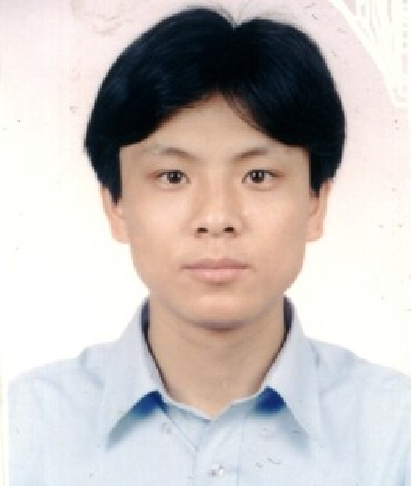
\includegraphics[width=1in,height=1.25in,clip,keepaspectratio]{Xiaofei}}]{Xiaofei Liao} received a Ph.D. degree in computer science and engineering from Huazhong University of Science and Technology (HUST), China, in 2005. He is now a Professor in school of Computer Science and Engineering at HUST. His research interests are in the areas of system virtualization, system software, and Cloud computing.
%\end{IEEEbiography}
%\vspace{-35pt}
%\begin{IEEEbiography}[{
\includegraphics[width=1in,height=1.25in,clip,keepaspectratio]{zhaojin}}]{Jin Zhao} received his bachelor degree in information security from China University of Geosciences, China, in 2017. He is now a doctoral student in school of computer science at Huazhong University of Science and Technology (HUST). His current research interests include graph processing, system software and architecture.
%\end{IEEEbiography}
%\vspace{-35pt}
%\begin{IEEEbiography} [{\includegraphics[width=1in,height=1.25in,clip,keepaspectratio]{Yu}}]{Yu Zhang} received a Ph.D. degree in computer science from Huazhong University of Science and Technology (HUST) in 2016. He is now an associate professor in school of computer science at HUST. His research interests include computer architecture, system software, runtime optimization, programming model, and big data processing. He is a member of the CCF, IEEE, ACM, and USENIX.
%\end{IEEEbiography}
%\vspace{-35pt}


%\begin{IEEEbiography} [{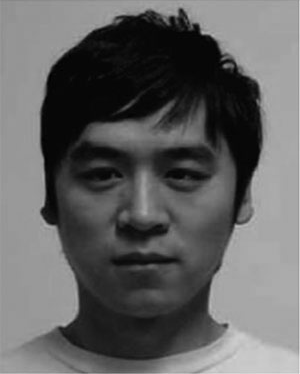
\includegraphics[width=1in,height=1.25in,clip,keepaspectratio]{Zeng}}]{Deze Zeng} received the BS degree from the School of Computer Science and Technology, Huazhong University of Science and Technology, China, in 2007 and the MS and PhD degrees in computer science from University of Aizu, Aizu-Wakamatsu, Japan, in 2009 and 2013, respectively. He is a full professor with the School of Computer Science, China University of Geosciences, Wuhan, China. His current research interests include network function virtualization, software-defined networking, cloud computing and edge computing. He has authored two books and more than 100 papers in refereed journals and conferences in these areas. He also received three best paper awards from IEEE/ACM conferences and the IEEE Systems Journal Annual Best Paper Award of 2017. He serves in editorial boards of the Journal of Network and Computer Applications, the Frontiers of Computer Science, and guest editors of many prestigious journals. He has been the in organization or program committees of many international conferences including ICPADS, ICA3PP, CollaberateCom, 	MobiQuitous, ICC, Globecom. He is a member of the IEEE.
%\end{IEEEbiography}
%\vspace{-35pt}


%\begin{IEEEbiography} [{\includegraphics[width=1in,height=1.25in,clip,keepaspectratio]{BingshengHe}}]{Bingsheng He} received the PhD degree from Hong Kong University of Science \& Technology, in 2008. He is currently an associate professor with the Department of Computer Science, National University of Singapore (NUS). Before joining NUS in 2016, he held a research position with the System Research group of MSRA (2008-2010) and a faculty position with Nanyang Technological University, Singapore. His research interests include big data management, parallel and distributed systems, and cloud computing.
%\end{IEEEbiography}
%\vspace{-35pt}
%\begin{IEEEbiography} [{\includegraphics[width=1in,height=1.25in,clip,keepaspectratio]{LigangHe}}]{Ligang He}  (Member, IEEE) is a Reader in the Department of Computer at the University of Warwick. He has published more than 130 articles in international conferences and journals, such as the IEEE TC, TPDS, TACO, IPDPS, ICPP, SC, VLDB. His research interests focus on parallel and distributed processing, cluster, high performance computing and cloud computing.
%\end{IEEEbiography}
%\vspace{-35pt}
%\begin{IEEEbiography} [{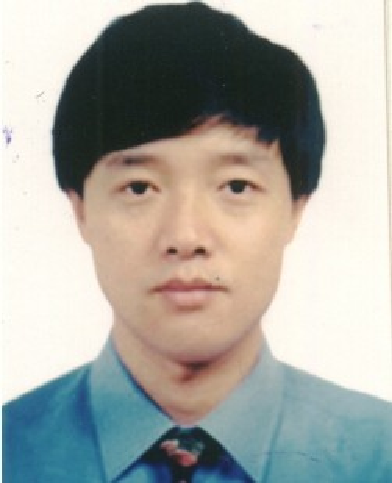
\includegraphics[width=1in,height=1.25in,clip,keepaspectratio]{Hai}}]{Hai Jin} is a Cheung Kung Scholars Chair Professor of computer science and engineering at Huazhong University of Science and Technology (HUST) in China. Jin received his PhD in computer engineering from HUST in 1994. In 1996, he was awarded a German Academic Exchange Service fellowship to visit the Technical University of Chemnitz in Germany. Jin worked at The University of Hong Kong between 1998 and 2000, and as a visiting scholar at the University of Southern California between 1999 and 2000. He was awarded Excellent Youth Award from the National Science Foundation of China in 2001. Jin is the chief scientist of ChinaGrid, the largest grid computing project in China, and the chief scientists of National 973 Basic Research Program Project of Virtualization Technology of Computing System, and Cloud Security. Jin is a Fellow of CCF, a Fellow of the IEEE and a member of the ACM. He has co-authored 22 books and published over 800 research papers. His research interests include computer architecture, virtualization technology, cluster computing and cloud computing, peer-to-peer computing, network storage, and network security.
%\end{IEEEbiography}
%\vspace{-35pt}
%\begin{IEEEbiography}[{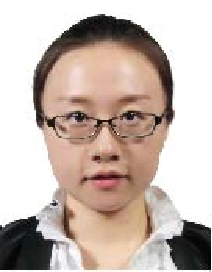
\includegraphics[width=1in,height=1.25in,clip,keepaspectratio]{LinGu}}]{Lin Gu} received her Ph.D. and M.S. degrees in computer science from University of Aizu, Fukushima, Japan, in 2015 and 2011, respectively. She received her B.S. degree from School of Computer Science and Technology, Huazhong University of Science and Technology, China in 2009. She is now with the Services Computing Technology and System Lab, Cluster and Grid Computing Lab in the School of Computer Science and Technology, Huazhong University of Science and Technology. Her current research interests include cloud computing, Big Data and Software-defined Networking.
%\end{IEEEbiography}

% if you will not have a photo at all

% You can push biographies down or up by placing
% a \vfill before or after them. The appropriate
% use of \vfill depends on what kind of text is
% on the last page and whether or not the columns
% are being equalized.

%\vfill

% Can be used to pull up biographies so that the bottom of the last one
% is flush with the other column.
%\enlargethispage{-5in}



% that's all folks
\end{document}


